\documentclass[twoside,10pt]{report}
\usepackage{blindtext,  fancyhdr}
\pagestyle{fancy}
\usepackage{a4wide}
\usepackage[T1]{fontenc}
\usepackage[utf8]{inputenc}
\usepackage{times}

\usepackage[font=small,labelfont=bf,tableposition=top]{caption}
\usepackage{graphicx}
\usepackage{natbib} 

\usepackage{amsmath}
\usepackage{amsfonts}
\usepackage{amssymb}
\usepackage{color, soul}
\usepackage{hyperref}
\usepackage{algorithmicx}
\usepackage{algpseudocode}
\usepackage{subfigure}
\usepackage{stmaryrd}

\renewcommand{\vec}[1]{\boldsymbol{{#1}}} 
\newcommand{\duesoon}[1]{{\sethlcolor{green}\hl{#1}}}
\usepackage{mathrsfs}


\newtheorem{theorem}{Theorem}
\newtheorem{acknowledgement}[theorem]{Acknowledgement}
\newtheorem{algorithm}[theorem]{Algorithm}
\newtheorem{axiom}[theorem]{Axiom}
\newtheorem{case}[theorem]{Case}
\newtheorem{claim}[theorem]{Claim}
\newtheorem{conclusion}[theorem]{Conclusion}
\newtheorem{condition}[theorem]{Condition}
\newtheorem{conjecture}[theorem]{Conjecture}
\newtheorem{corollary}[theorem]{Corollary}
\newtheorem{criterion}[theorem]{Criterion}
\newtheorem{definition}[theorem]{Definition}
\newtheorem{example}[theorem]{Example}
\newtheorem{exercise}[theorem]{Exercise}
\newtheorem{lemma}[theorem]{Lemma}
\newtheorem{notation}[theorem]{Notation}
\newtheorem{problem}[theorem]{Problem}
\newtheorem{proposition}[theorem]{Proposition}
\newtheorem{remark}[theorem]{Remark}
\newtheorem{solution}[theorem]{Solution}
\newtheorem{summary}[theorem]{Summary}
\newenvironment{proof}[1][Proof]{\textbf{#1.} }{\ \rule{0.5em}{0.5em}}

\newtheorem{guess}{Definition}
\newcommand{\comment}[1] {}
\newcommand{\Norder} {N}
\newcommand{\order}{\mathcal{O}}
\newcommand{\Npoints} {N_p}
\newcommand{\Nfaces} {N_{f}}
\newcommand{\Nelements} {N_e}

\newcommand{\eps}{\varepsilon}
\newcommand{\Dweak}{\wt{D}}
\newcommand{\diff}[2] {\frac{\partial #1}{\partial #2}}
\newcommand{\dxx}[2] {\frac{\partial^2 #1}{\partial {#2}^2}}
\newcommand{\difft}[2] {\frac{d #1}{d #2}}
\newcommand{\dxxt}[2] {\frac{d^2 #1}{d {#2}^2}}
\newcommand{\lagrange}[1] {\frac{d #1}{dt}}
\newcommand{\lebesgue}{\parallel I \parallel}
\newcommand{\polysp}{\mathcal{P}_N}
\newcommand{\laplacian}{\nabla^2}
\newcommand{\divergence}{\nabla \cdot}
\newcommand{\inte}{\int_{\mbox{\footnotesize ${\Omega_e}$}}}
\newcommand{\intb}{\int_{\mbox{\footnotesize ${\Gamma_e}$}}}
\newcommand{\intce}{\int_{\mbox{\footnotesize ${\widehat{\Omega}_e}$}}}
\newcommand{\intcb}{\int_{\mbox{\footnotesize ${\widehat{\Gamma}_e}$}}}
\newcommand{\intg}{\int_{\mbox{\footnotesize ${\Omega}$}}}
\newcommand{\intgb}{\int_{\mbox{\footnotesize ${\Gamma}$}}}
\newcommand{\intv}{\int_{\mbox{\footnotesize ${\sigma}$}}}
\newcommand{\sumv}{\sum_{K=1}^{N_{\mathrm{lev}}}}
\newcommand{\sumk}{\sum_{L=1}^{K}}
\newcommand{\sumN}{\sum_{i=1}^{N+1}}
\newcommand{\half}{\frac{1}{2}}
\newcommand{\inti}{\int_{\mbox{\footnotesize\sf I}}}
\newcommand{\intbd}{\oint_{\mbox{\footnotesize ${\delta}$\sf D}}}
\newcommand{\intbi}{\oint_{\mbox{\footnotesize ${\delta}$\sf I}}}
\newcommand{\ldnorm}[1]{\left\| #1 \right\|_{\mbox{\footnotesize \sf D}} }
\newcommand{\lonorm}[1]{\left\| #1 \right\|_{\Omega}}
\newcommand{\spc}[1]{\mbox{\sf #1}}
\newcommand{\ope}[1]{{\cal #1}}
\newcommand{\mt}[1]{{\rm #1}}
\newcommand{\dis}{\displaystyle}
\newcommand{\ve}{\varepsilon}
\newcommand{\ov}{\overline}
\newcommand{\wt}{\widetilde}
\newcommand{\wh}{\widehat}
\newcommand{\Dhat}{\widehat{D}}
\newcommand{\be}{\begin{equation}}
\newcommand{\ee}{\end{equation}}
\newcommand{\bea}{\begin{eqnarray*}}
\newcommand{\eea}{\end{eqnarray*}}
\newcommand{\Jace}{J^{(e)}}
\newcommand{\Jacl}{J^{(l)}}
\def\bepsilon{\mbox{\boldmath $\epsilon $}}
\def\bpsi{\mbox{\boldmath $\psi $}}
\def\bphi{\mbox{\boldmath $\phi $}}
\def\bmu{\mbox{\boldmath $\mu $}}
\def\Et{ \tilde{E} }
\def\Ht{ \tilde{H} }
\def\sdot{ \dot{\sigma} }

\newcommand{\fstar}{f^{(*)}}

\DeclareMathOperator{\Span}{span}
\DeclareMathOperator{\Dim}{dim}

\newcommand{\polyquad}{\mathcal{Q}_{N}}
\newcommand{\polyP}{\mathcal{P}_{N}}
\newcommand{\polyPnpm}{\mathcal{P}_{(N+M)}}
\newcommand{\polyPd}{\mathcal{P}_{d}}
\newcommand{\polyPnm}{\mathcal{P}_{N,M}}
\newcommand{\polyPn}{\mathcal{P}_{N,0}}
\newcommand{\transpose}{^{\mathcal{T}}}

\newcommand{\vecQ}{\vec{Q}}
\newcommand{\vecQe}{\vec{Q}^{(e)}}
\newcommand{\vecFe}{\vec{\mathcal{F}}^{(e)}}
\newcommand{\statevec}{\vec{Y}}
\newcommand{\statevecN}{\vec{Y}_N^{(e)}}
\newcommand{\statestage}{\vec{\mathcal{Y}}}
\newcommand{\Ftensor}{\vec{F}(\qvector)}
\newcommand{\FtensorN}{\vec{F}\left( \qvectorN \right)}
\newcommand{\FtensorStar}{\vec{F}\left( \qvector_N^{(e,k)} \right)}
\newcommand{\Svector}{S(\qvector)}
\newcommand{\SvectorN}{S \left( \qvectorN \right)}
\newcommand{\qref}{\vec{q}_0}
\newcommand{\qvectorb}{\vec{q}_b}
\newcommand{\qtt}{\vec{q}_{tt}}
\newcommand{\qhat}{\widehat{\vec{q}}}
\newcommand{\qhatb}{\widehat{\vec{q}}_b}
\newcommand{\qelem}{q^{(e)}}
\newcommand{\rhoref}{\rho_0}
\newcommand{\piref}{\pi_0}
\newcommand{\Thetaref}{\Theta_0}
\newcommand{\Gref}{G_0}
\newcommand{\Tref}{T_0}
\newcommand{\thetaref}{\theta_0}
\newcommand{\Pref}{{P}_0}
\newcommand{\Eref}{{E}_0}
\newcommand{\Href}{{h}_0}
\newcommand{\rhohat}{\widehat{\rho}}
\newcommand{\pihat}{\widehat{\pi}}
\newcommand{\Phat}{\widehat{P}}
\newcommand{\uvechat}{\widehat{{\mbox{\boldmath$u$\unboldmath}}}}
\newcommand{\uhathat}{\widehat{\widehat{{\mbox{\boldmath$u$\unboldmath}}}}}
\newcommand{\Uhat}{\widehat{{\mbox{\boldmath$U$\unboldmath}}}}
\newcommand{\Uhathat}{\widehat{\widehat{{\mbox{\boldmath$U$\unboldmath}}}}}
\newcommand{\thetahat}{\widehat{\theta}}
\newcommand{\Thetahat}{\widehat{\Theta}}
\newcommand{\Ehat}{\widehat{E}}
\newcommand{\uhat}{\widehat{u}}
\newcommand{\vhat}{\widehat{v}}
\newcommand{\what}{\widehat{w}}
\newcommand{\pitt}{\pi_{tt}}
\newcommand{\rhott}{\rho_{tt}}
\newcommand{\Ett}{E_{tt}}
\newcommand{\Utt}{\vec{U}_{tt}}
\newcommand{\uvectt}{\vec{u}_{tt}}
\newcommand{\utt}{u_{tt}}
\newcommand{\vtt}{v_{tt}}
\newcommand{\wtt}{w_{tt}}
\newcommand{\Ptt}{P_{tt}}
\newcommand{\vecPtt}{\vec{P}_{tt}}
\newcommand{\Thetatt}{\Theta_{tt}}
\newcommand{\thetatt}{\theta_{tt}}
%Projector Matrices
\newcommand{\projmatrix}{\vec{\mathcal{P}}}
\newcommand{\qmatrix}{\vec{\mathcal{Q}}}
\newcommand{\pcmatrix}{\vec{\mathcal{P}}_C}
\newcommand{\Cmatrix}{\left(\vec{\mathcal{C}}^{(e,f)}\right)\transpose}
\newcommand{\Dmatrix}{\vec{D}^{(e)}}
\newcommand{\Dwmatrix}{\wt{\vec{D}}^{(e)}}
\newcommand{\Mmatrix}{M^{(e)}}
\newcommand{\Fmatrix}{\vec{F}^{(e,l)}}
\newcommand{\Gmatrix}{\mathcal{G}}
\newcommand{\Umatrix}{\mathcal{U}^{(e,f)}}
\newcommand{\amatrix}{\vec{\mathcal{A}}}
\newcommand{\rmatrix}{\vec{\mathcal{R}}}
%Vectors
\newcommand{\nvector}{\wh{\vec{n}}_{\Gamma}}
\newcommand{\nhat}{\wh{\vec{n}}}
\newcommand{\ivector}{\wh{\vec{i}}}
\newcommand{\jvector}{\wh{\vec{j}}}
\newcommand{\kvector}{\wh{\vec{k}}}
\newcommand{\rvector}{\wh{\vec{r}}}
\newcommand{\svector}{\wh{\vec{s}}}
\newcommand{\tvector}{\wh{\vec{t}}}
\newcommand{\vvector}{\wh{\vec{v}}}
\newcommand{\Qvector}{\vec{Q}}
%Vectors
\newcommand{\ur}{{u}^{(r)}}
\newcommand{\us}{{u}^{(s)}}
\newcommand{\ut}{{u}^{(t)}}
\newcommand{\urtt}{{u}_{tt}^{(r)}}
\newcommand{\ustt}{{u}_{tt}^{(s)}}
\newcommand{\uttt}{{u}_{tt}^{(t)}}
\newcommand{\urhat}{\widehat{u}^{(r)}}
\newcommand{\ushat}{\widehat{u}^{(s)}}
\newcommand{\uthat}{\widehat{u}^{(t)}}
%Other Operators
\newcommand{\grad}{\vec{\nabla}}
\newcommand{\Grad}{\vec{\nabla}}
\newcommand{\Dskew}{\mathcal{D}}

\def\bepsilon{\mbox{\boldmath $\epsilon $}}
\def\bpsi{\mbox{\boldmath $\psi $}}
\def\bphi{\mbox{\boldmath $\phi $}}
\def\bmu{\mbox{\boldmath $\mu $}}
\def\Et{ \tilde{E} }
\def\Ht{ \tilde{H} }
\def\sdot{ \dot{\sigma} }
%\renewcommand{\thetable}{\Roman{table}}
%\renewcommand{\thefigure}{\arabic{figure}}

%\DeclareMathOperator{\Span}{span}
%\DeclareMathOperator{\Dim}{dim}

%Editing Commands
\newcommand{\here}{ \textcolor{red}{YOU ARE HERE}}

%Time-Integration
\newcommand{\dt}{{\Delta t}}
\newcommand\ST{\rule[-0.75em]{0pt}{2em}}
\newcommand{\Sfunction}{\mathcal{S}}
\newcommand{\Lfunction}{\mathcal{L}}
\newcommand{\Nfunction}{\mathcal{N}}

%DG Operators
\newcommand{\average}[1]{ \left\{ #1 \right\} }
\newcommand{\jump}[1]{ \llbracket #1 \rrbracket }

%HDG Matrices
\newcommand{\CCmatrix}{\mathcal{C}^{(e,k)}}
\newcommand{\Jmatrix}{\mathcal{J}^{(e,k)}}
\newcommand{\DDmatrix}{\wt{D}^{(e)}}
\newcommand{\SSvector}{\mathcal{S}(q)}
\newcommand{\cghdg}{cg\underline{\hspace{0.15cm}}to\underline{\hspace{0.15cm}}hdg}
%\newcommand{\ul}{\underline{\hspace{0.15cm}}}
\newcommand{\RRmatrix}{\mathcal{R}}

%Clima specific variables
\newcommand{\etotal}{e^{\mathrm{tot}}}
\newcommand{\Etotal}{E^{\mathrm{tot}}}
\newcommand{\Fvector}{\vec{\mathcal{F}}}
\newcommand{\Pvector}{\vec{\mathcal{P}}}
\newcommand{\Fadv}{\vec{\mathcal{F}}^{\mathrm{adv}}}
\newcommand{\Fndf}{\vec{\mathcal{F}}^{\mathrm{ndf}}}
\newcommand{\Fdiff}{\vec{\mathcal{F}}^{\mathrm{diff}}}
\newcommand{\Tvector}{\vec{\mathcal{T}}}
\newcommand{\Source}{\vec{\mathcal{S}}}

\newcommand{\fxg}[1]{\textcolor{cyan}{FXG: #1}}




\title{CLIMA Land Model} 

\author{ }

\begin{document}

\maketitle
\tableofcontents

\chapter{Purpose, Goals, and Non-Goals}

\section{Overview}

This document describes the scientific concepts underlying the CLIMA land model. It lays out a consistent set of equations governing components of the land model such as soil, snow, and vegetation, and it discusses the boundary conditions through which the land model couples to the atmosphere. The land model is built upon these concepts and equations and is designed to be coupled to the CLIMA atmosphere model or run in standalone mode (e.g., driven by reanalysis data). Because the land model is part of a climate model, conservation of energy, water, and carbon are essential, both within the land model and in exchanges with the atmosphere. Figure~\ref{f:land_model_schematic} provides a schematic of the land model components and how they interact with each other and with the atmosphere and ocean models. Table~\ref{tab:LM-modules} summarizes the model components and their inputs, outputs, and functional requirements, which are discussed in detail in this document.\hl{[update figure and table]}
\begin{figure}[htb]
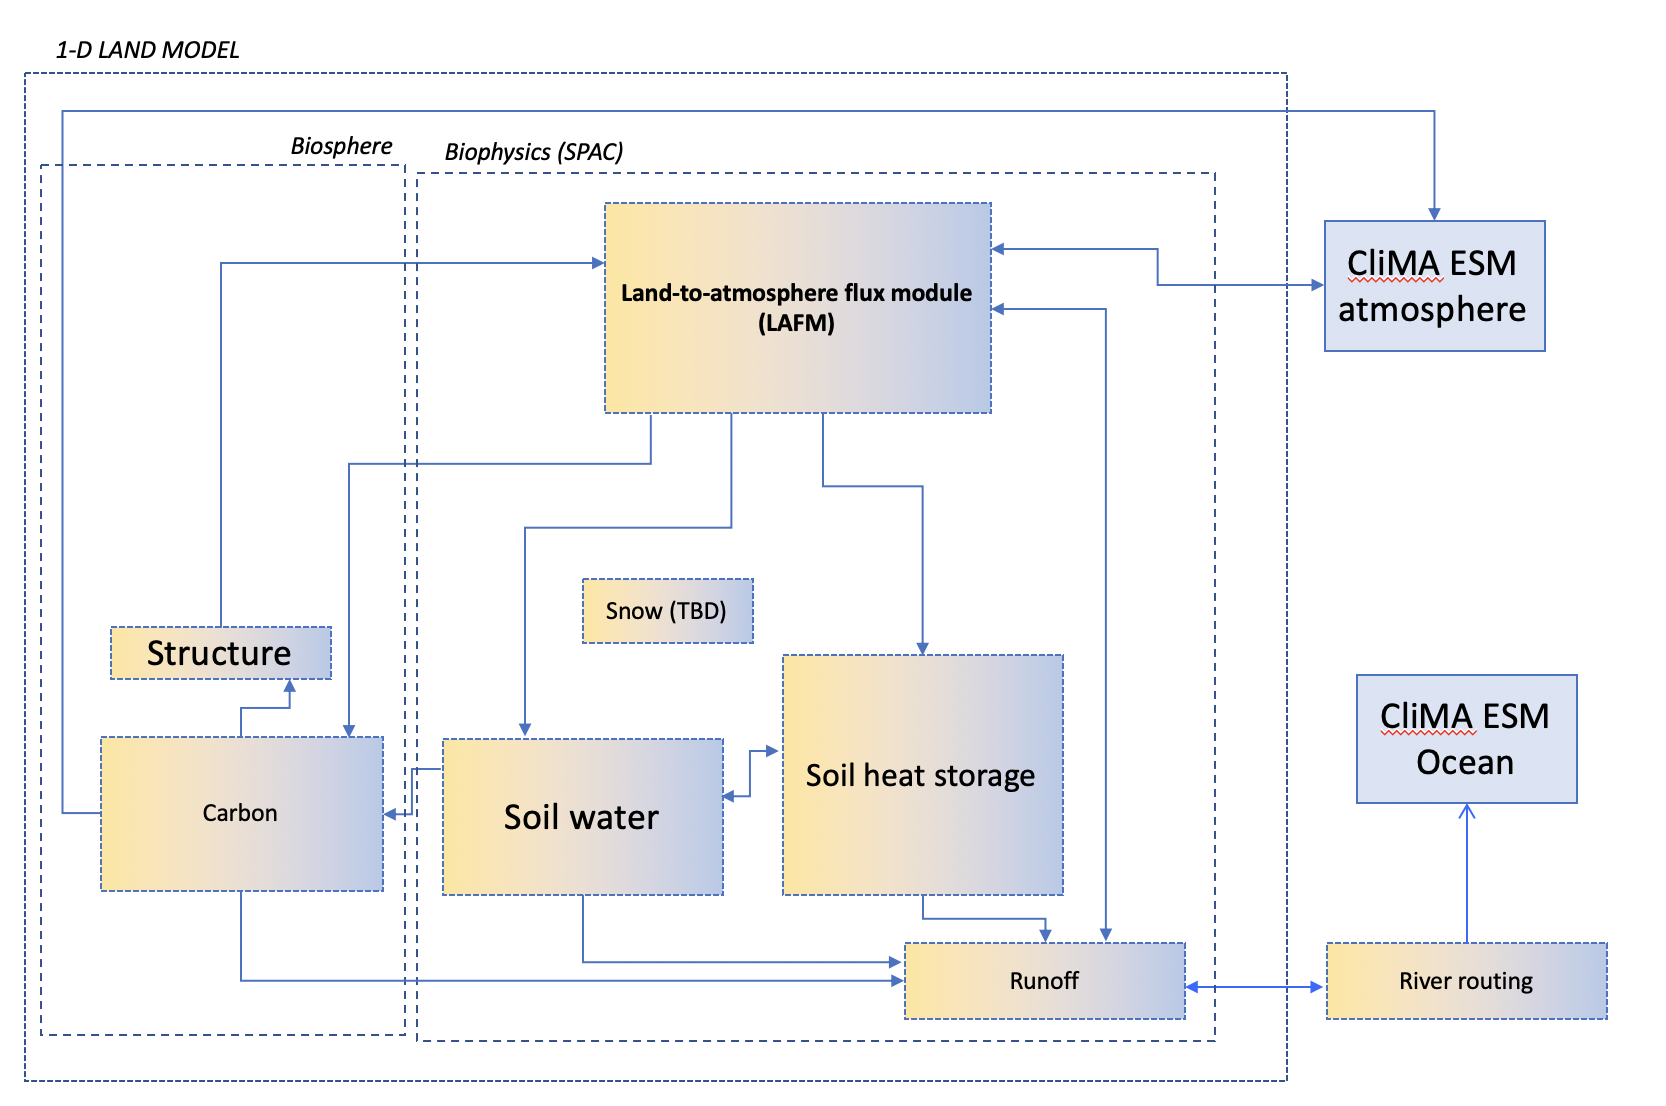
\includegraphics[width=10cm,height=10cm,keepaspectratio]{CLIMA-land/LM_figures/JPLCLIMA_LM_DESIGN_20191115.png}
\caption{Schematic of land model components and their internal and external dependencies. Model components interact with each other; for example, the canopy model interacts with the soil model through source/sink terms representing processes such as water uptake by roots, and it interacts with turbulent fluxes in the atmospheric near-surface layer through exchange of momentum, energy, and water. \hl{[ALL: please comment + suggest improvements; Pierre's comment: SPAC should include all biophysics, re-name/re-arrange/simplify boxes]}}
\label{f:land_model_schematic}
\end{figure}
% Please add the following required packages to your document preamble:
% \usepackage{graphicx}
\begin{table}[]
\resizebox{\textwidth}{!}{%
\begin{tabular}{|l|l|l|l|}
\hline
Module [code]         & Input requirements [From]                                                                & Output requirements                                                       & Module requirements                      \\ \hline
Carbon [C]            & \begin{tabular}[c]{@{}l@{}}GPP [F], \\ Soil water profile [W], \\ Soil temperature profile [E]\end{tabular}                                                               & \begin{tabular}[c]{@{}l@{}}Carbon states\\ (Biomass, inc. foliar, roots, wood;\\ Dead organic C) \\ Carbon fluxes \\ (respiration, disturbance fluxes)\end{tabular} & \begin{tabular}[c]{@{}l@{}}The carbon module will calculate \\ internal land biosphere carbon transfers \\ (allocation, mortality, mineralization), \\ and gross land-atmosphere C fluxes \\ (respiration, fires)\end{tabular} \\ \hline

Structure [S]         & Biomass [C]                                                             & \begin{tabular}[c]{@{}l@{}}Biophysical states:\\ Canopy height, Chlorophyll, \\Root profile, LMA\end{tabular}                                                        &                                                                   \\ \hline
Soil water [H]        & \begin{tabular}[c]{@{}l@{}}Soil freeze/thaw state [E] \\ Precipitation [A]\\ Evaporation [F], \\ Transpiration (vertically resolved), \\ root profile [S]\end{tabular} &
\begin{tabular}[c]{@{}l@{}}
Vertical soil water states\\Soil water fluxes\\Runoff\end{tabular}                                                                                                                  & \begin{tabular}[c]{@{}l@{}}Module will calculate vertical \\ water flow in soil Darcy’s law, \\ Richards' equations, hydraulic \\redistribution,  runoff, etc.\end{tabular}                                                     \\ \hline
Soil heat storage [E] & Soil water [H], Precip. temp [A]
& 
\begin{tabular}[c]{@{}l@{}}
Vertical temperature profile\\
Runoff temperature       \end{tabular}                                               &                                                                                                \\ \hline
%%%%%%(SPAC-Flux)%%%%%
\begin{tabular}[c]{@{}l@{}}
Land-to-atmosphere\\ fluxes [F]  \\
(previously SPAC-Flux)
\end{tabular}

        & \begin{tabular}[c]{@{}l@{}}Atmospheric variables [A], \\ Biophysical states[S], \\ Soil water profile [H], \\ Soil energy profile [E],\end{tabular}                   & \begin{tabular}[c]{@{}l@{}}Land-surface Fluxes\\ GPP, evapotranspiration, H, $\lambda$E, radiative fluxes \end{tabular}                                 & 

\begin{tabular}[c]{@{}l@{}} Canopy P interception\\ Radiative transfer in canopy     \end{tabular}                                                        \\ \hline

River routing [R]        & \begin{tabular}[c]{@{}l@{}} Soil runoff [H], \\ CliMA Ocean [O] \end{tabular}                             & \begin{tabular}[c]{@{}l@{}} River Discharge\end{tabular}                                             &                                     \\ \hline \hline \hline


CliMA Atmosphere [A]        & \begin{tabular}[c]{@{}l@{}}Land surface fluxes [F], \\ Land biosphere fluxes [C]\end{tabular}                             & \begin{tabular}[c]{@{}l@{}}Atmospheric variables [for land]\\ Radiative fluxes, precipitation, temperature, humidity,\end{tabular}                                             &                                     \\ \hline

CliMA Ocean [O]        & \begin{tabular}[c]{@{}l@{}}River discharge [R] \end{tabular}                             & \begin{tabular}[c]{@{}l@{}} Ocean variables (for land) Sea Level\end{tabular}                                             &                                     \\ \hline
\end{tabular}}
\caption{\label{tab:LM-modules}Overview of inputs, outputs, and functional requirements of land model components.}
\end{table}

Chapter~\ref{c:soil} begins with a description of the soil model and its treatment of the energy and water balance of soil. \hl{[add rest of overview]}.

\section{Goals}

\begin{itemize}
    \item Provide a complete and self-contained documentation of the scientific concepts underlying the land model.
    \item Establish a consistent notation for the governing equations, which may guide data structures and variable names in the code.
    \item Establish a consistent set of approximations for the governing equations that allow the land model to be used both on climate model scales (tens of kilometers and larger) and large-eddy simulation (LES) scales (kilometers and smaller).
    \item Describe boundary conditions that ensure conservation of energy, water, and tracer (e.g., carbon) masses during exchanges with other climate model components, while treating the interfacial layer (e.g., near-surface turbulence in the atmosphere) consistently across model components.
    \item Harmonize equations and boundary conditions to facilitate coupling with the \href{https://github.com/climate-machine/Design-Docs/blob/master/CLIMA-atmos/}{CLIMA atmosphere} model.
    \item Lay out the concepts in a way that can be directly translated into code. Key equations that appear in the code are highlighted in \hlpaleblue{blue boxes}.
    \item Document benchmark cases for testing the land model.
\end{itemize}

\section{Non-Goals}

\begin{itemize}
    \item Discuss software architecture and data structures.
    \item Discuss numerical methods in detail.
    \item Discuss implementation details such as variable names and computational aspects.
\end{itemize}
These are covered in the separate design documents, on \href{https://github.com/climate-machine/Design-Docs/tree/master/CLIMA-numerics}{numerical methods} and software. \hl{[TBW, link]}.

\chapter{Soil Physics}\label{c:soil}

The soil model represents the transport of energy and moisture in soil, links them to atmospheric boundary conditions above, and provides water input for runoff models (e.g., along the surface or in rivers). Vegetation is linked to the soil model through root extraction, which represents water sources and sinks in soil, and through modulation of radiation reaching the top of the soil.  This chapter describes the energy and water balances in soil and how atmospheric boundary conditions and vegetation link to them.

\section{Composition of Soil}

\subsection{Bulk Soil}

We take soil to consist of a dry soil matrix (composed of sand, clay, rock, etc.) with pore spaces that may contain liquid water, ice, and gases (air with water vapor). The bulk density of the soil mixture, including water, is $\rho$ ($\mathrm{kg~m^{-3}}$). The composition of soil is characterized by mass fractions (mass of constituent divided by total mass of soil), which each depend on a space coordinate and time:
\begin{itemize}
    \item $q_{ds}$: mass fraction of dry soil,
    \item $q_l$: mass fraction of liquid water,
    \item $q_i$: mass fraction of ice,
    \item $q_w = q_l + q_i$: mass fraction of total water (liquid and ice).
\end{itemize}
We neglect the small mass (but not the volume) of gases in pore spaces, so that this enumerates all constituents of soil that contribute to soil mass; therefore, 
\[
q_{ds} + q_l + q_i = q_{ds} + q_w = 1.
\]

Because the primary constituents of soil are essentially incompressible, the composition of soil is commonly expressed in terms of volume fractions (e.g., volume of liquid water per volume of soil). The volume fractions $\theta_{\cdot}$ of the constituents are related to the mass fractions $q_{\cdot}$ through
\begin{subequations}\label{e:vol_fractions}
\begin{align}
    \theta_{ds} &= \frac{q_{ds} \rho}{\rho_{ds}} \\
    \theta_l &= \frac{q_l \rho}{\rho_l}, \\
    \theta_i &= \frac{q_i \rho}{\rho_i}, \\
    \theta_w &= \theta_l + \theta_i.
\end{align}
\end{subequations}
Here, $\rho_{ds}$ is the particle density of dry soil (i.e., the density of the soil particles alone, without pore spaces), and $\rho_l$ and $\rho_i$ are the densities of liquid water and ice, respectively. We take liquid water to be incompressible, and the densities $\rho_l$ of liquid and $\rho_i$ of ice to be constant. The density variations of liquid water are of order $10^{-3}$ over typical soil temperatures, which is negligible compared with other variations, for example, of the viscosity of liquid water. We summarize the water content of soil by the  tuple $\vec{\theta} = (\theta_l, \theta_i)$.

While the mass fractions of dry soil and water sum to one, the volume fractions do not: Gases, which are assumed to have zero mass, occupy a volume fraction $\theta_g = 1 - (\theta_{ds} + \theta_w)$. Gases, liquid water, and ice occupy pore spaces in the soil matrix. The volume fraction of pore spaces that can be filled with either gas or water is the porosity 
\begin{equation}\label{e:porosity}
    \nu_p = \theta_g + \theta_w =  1 - \theta_{ds}.
\end{equation}
The porosity is the volume fraction filled with gas when the soil is dry ($\theta_w=0$), or it is the volume fraction occupied by liquid water when all voids are filled with liquid water ($\theta_g = \theta_i = 0$). 

\subsection{Dry Soil}

The dry soil portion of the bulk soil in turn consists of constituents such as mineral soil, gravel, organic matter, or bedrock, which all have different thermodynamic and hydraulic properties.  Let $\nu_{i}$ indicate the dry volume fraction of constituent $\chi_i$ in the total volume of soil, with $\chi_i$ labeling the constituents, for example,
\[
\chi_i \in \{ {\mathrm{sand}}, {\mathrm{clay}}, {\mathrm{silt}}, {\mathrm{gravel}}, \mathrm{organic~matter}, {\mathrm{bedrock}} \}.
\]
We include bedrock in the soil constituents to be able to directly apply our soil model in bedrock, simply by modifying location-specific (3D) thermodynamic and hydraulic parameters. If the $\nu_i$'s enumerate all constituents of dry soil, the volume fractions sum to the total dry-soil volume fraction $1-\nu_p$,
\[
\sum_i \nu_{i} = 1-\nu_p.
\] 
We use the tuple $\vec{\nu} = (\nu_p, \nu_i)$ to summarize the composition of dry soil, including its porosity $\nu_p$. The dry soil composition depends on a space coordinate, and it may also vary on long (decadal and longer) timescales.

\subsection{Soil Density}

The dry particle density of dry soil is the weighted mean of the dry particle densities $\rho_{\chi_i}$ of the constituents $\chi_i$:
\begin{equation}\label{d:dry_soil_density}
    \rho_{ds}(\vec{\nu})  = (1-\nu_p)^{-1} \sum_i \nu_{i} {\rho}_{\chi_i}.
\end{equation}
This gives the bulk soil density, including the water contained in the soil,  
\begin{equation}\label{e:bulk_density}
\rho (\vec{\theta}; \vec{\nu}) = (1-\nu_p) \rho_{ds} + \theta_l \rho_l + \theta_i \rho_i,
\end{equation}
which follows from the definition of the volume fractions \eqref{e:vol_fractions} and of porosity \eqref{e:porosity}. 

\section{Heat Capacity of Soil}

\subsection{General Formulation}

The specific heat capacity of soil (heat capacity per unit mass, $\mathrm{J~kg^{-1}~K^{-1}}$) is the mass-weighted sum of the specific heat capacities of the constituents
\begin{equation}\label{e:soil_specific_heat}
    c_s = (1-q_w) c_{ds} + q_l c_{l} + q_i c_{i},
\end{equation}
where we have used $q_{ds} = 1 - q_w$ and the specific heat capacities of the constituents are:
\begin{itemize}
    \item $c_{ds}$: Specific heat capacity of dry soil,
    \item $c_l$: Specific heat capacity of liquid water,
    \item $c_i$: Specific heat capacity of ice.
\end{itemize}
Consistent with neglecting the mass of the gas constituents, we neglect their contribution to the soil specific heat capacity.

The specific heat capacity of dry soil depends on spatially varying soil properties (discussed below). We take the specific heat capacities of liquid water and ice to be constants, consistent with the thermodynamics of the  \href{https://github.com/climate-machine/Design-Docs/blob/master/CLIMA-atmos/}{CLIMA atmosphere} model. These constants should be chosen to be the same in atmosphere, ocean, land, and other models; they are set in the \href{https://github.com/climate-machine/CLIMA/tree/master/src/Common/PlanetParameters}{PlanetParameters} module \hl{[update link]}.

Because, as is common, we use volume fractions to characterize the composition of the soil, we also use the volumetric heat capacities (heat capacities per unit volume, $\mathrm{J~m^{-3}~K^{-1}}$):
\begin{subequations}\label{e:vol_heat_capacities}
\begin{align}
    \tilde{c}_{ds} &= \rho_{ds} c_{ds},\\
    \tilde{c}_{l} &= \rho_{l} c_{l},\\
    \tilde{c}_{i} &= \rho_{i} c_{i}.
\end{align}
\end{subequations}
In terms of volume fractions of constituents, the combined volumetric heat capacity of soil is the weighted mean
\begin{equation}\label{e:soil_spec_heat_volume_0}
    \tilde c_s = \rho c_s = (1-\nu_p) \tilde c_{ds} + \theta_l \tilde c_l + \theta_i \tilde c_i.
\end{equation}
This expression for the volumetric heat capacity follows by substituting the definitions of volume fractions \eqref{e:vol_fractions}, porosity \eqref{e:porosity}, and volumetric heat capacities \eqref{e:vol_heat_capacities} into the definition of the specific heat capacity of soil \eqref{e:soil_specific_heat}. Instead of referring the heat capacity of dry soil to a unit volume of solid soil only (excluding the pore space volume), it is convenient to use a bulk heat capacity of a volume of dry soil that includes the pore space volume:
\begin{equation}\label{e:bulk_dry_heat_capacity0}
    \check{c}_{ds}(\vec{\nu}) = (1-\nu_p) \tilde{c}_{ds}.
\end{equation}
In terms of this bulk volumetric heat capacity of dry soil, the volumetric heat capacity of soil \eqref{e:soil_spec_heat_volume_0} becomes
\begin{empheq}[box=\eqnbox]{equation}\label{e:soil_spec_heat_volume}
    \tilde c_s (\vec{\theta}; \vec{\nu}) = \check c_{ds}(\vec{\nu}) + \theta_l \tilde c_l + \theta_i \tilde c_i,
\end{empheq}
which is a function of the soil composition: it depends on water content  $\vec{\theta}$ (a model state variable) and parametrically on the dry-soil composition $\vec{\nu}$. The expression \eqref{e:soil_spec_heat_volume} makes it clear that the heat capacity of soil increases when pore spaces are filled with soil water. (Here and throughout this document, we use tilde and check accents to indicate thermodynamic quantities referenced to volume rather than mass.) 

\subsection{Heat Capacity of Dry Soil}

The volumetric heat capacity of dry soil is commonly approximated as the weighted mean of the volumetric heat capacities of mineral soil, gravel, organic matter, bedrock, and possibly other constituents \citep{Farouki81a}. If ${\tilde c}_{\chi_i}$ denotes the volumetric heat capacity of constituent $\chi_i$, the volumetric heat capacity of dry soil is the weighted mean 
\begin{equation}\label{e:dry_soil_heat_capacity}
\tilde{c}_{ds} (\vec{\nu}) = (1-\nu_p)^{-1} \sum_i \nu_{i} {\tilde c}_{\chi_i}.
\end{equation}
This is the volumetric heat capacity of the solid components of dry soil only, that is, excluding the pore space volume. The bulk heat capacity of a volume of dry soil that includes the pore space volume is
\begin{equation}\label{e:bulk_dry_heat_capacity}
    \check{c}_{ds} (\vec{\nu})  = (1-\nu_p) \tilde{c}_{ds} = \sum_i \nu_{i} {\tilde c}_{\chi_i}.
\end{equation}
This bulk dry heat capacity is commonly tabulated. 

Sources of the data needed to specify soil composition $\vec{\nu}$ and heat capacities $\check c_{ds}$ are listed in section~\ref{s:soil_data}.

\section{Thermodynamic State of Soil}

\subsection{Internal Energy}

We characterize the thermodynamic state of soil by its internal energy. The specific internal energy (energy per unit mass, $\mathrm{J~kg^{-1}}$) is the mass-weighted mean of the constituent specific internal energies of dry soil $I_{ds}$, liquid water $I_l$, and ice $I_i$,
\begin{equation}\label{e:energy_soil}
    I = (1-q_w) I_{ds} + q_l I_l + q_i I_i.
\end{equation}
Gases are again neglected, consistent with neglecting their mass. The specific internal energies of the constituents depend on the temperature $T$ of the constituents (which are assumed to be in local thermal equilibrium, so they have the same temperature in any one location) and the specific heat capacities:
\begin{subequations}\label{e:soil_internal_energies}
\begin{align}
I_{ds}(T; \vec{\nu}) & = c_{ds}(\vec{\nu}) (T - T_0),  \\
I_l(T) & = c_{l} (T - T_0), \\
I_i(T) & = c_{i} (T - T_0) - I_{i,0}.
\end{align}
\end{subequations}
The temperature $T_0$ is a reference temperature at which the specific internal energy of soil and liquid water are taken to vanish, and $I_{i,0}$ is the difference in specific internal energy between ice and liquid water at $T_0$. As is common for condensed phases (liquids and solids), we equate the internal energies and enthalpies of liquid water and ice, and approximate the specific internal energy difference $I_{i,0}$ by the specific enthalpy difference at $T_0$, which is the specific latent heat of fusion $L_{f,0}$ at $T_0$: 
\begin{equation}
    I_{i,0} = L_{f,0}.
\end{equation} 
These definitions for the internal energy of soil are consistent with those for the \href{https://github.com/climate-machine/Design-Docs/blob/master/CLIMA-atmos/}{CLIMA atmosphere} model. The reference temperature $T_0$ is arbitrary, but the specific latent heat of fusion $L_{f,0}$ must be chosen as that at $T_0$. The thermodynamic properties of water must be chosen to be the same for soil, atmosphere, and other model component, to ensure thermodynamic consistency. 

For the soil model, it is again convenient to use internal energies per unit volume ($\mathrm{J~m^{-3}}$) rather than the internal energies per unit mass. The internal energies per unit volume are related to the specific internal energies by
\begin{subequations}
\begin{align}
    \tilde I_{ds} &= \rho_{ds} I_{ds},\\
    \tilde I_{l}  &= \rho_{l} I_{l},\\
    \tilde I_{i}  &= \rho_{i} I_{i}.
\end{align}
\end{subequations}
Using the fact that the specific heat capacity of soil \eqref{e:soil_specific_heat} is the weighted mean of those of the constituents, together with the relation \eqref{e:soil_spec_heat_volume} for the volumetric specific heat, and the definition \eqref{e:vol_fractions} of the volume fractions, the total internal energy per unit volume can be written as
\begin{empheq}[box=\eqnbox]{equation}\label{e:vol_internal_energy}
\begin{split}
    \tilde I(T, \vec{\theta}; \vec{\nu})  &= \rho I 
    = \theta_{ds} \tilde I_{ds}(T; \vec{\nu}) + \theta_l  \tilde I_l(T) + \theta_i  \tilde I_i(T)\\
    &= \tilde{c}_s(\vec{\theta}; \vec{\nu}) (T - T_0) - \theta_i \rho_i L_{f,0}.
\end{split}
\end{empheq}
The internal energy $\tilde I$ of soil depends on temperature $T$ and, through the volumetric specific heat $\tilde c_s(\vec{\theta}; \vec{\nu})$, on water content $\vec{\theta}$ and dry-soil composition $\vec{\nu}$, the latter being a location-dependent parameter (section~\ref{s:soil_data}).

\subsection{Temperature}

Given the internal energy $\tilde I$ and composition ($\vec{\theta}; \vec{\nu}$) of the soil, the definition \eqref{e:vol_internal_energy} can be inverted to give the soil temperature
\begin{empheq}[box=\eqnbox]{equation}%\begin{equation}
\label{e:temperature_from_I}
    T = T_0 + \frac{\tilde{I} + \theta_i \rho_i L_{f,0}}{\tilde{c}_s(\vec{\theta}; \vec{\nu})}.
%\end{equation}
\end{empheq}
Thus, we can use the internal energy $\tilde I$ as a prognostic variable in a soil model and obtain the temperature $T$ from that and from knowledge of the composition ($\vec{\theta}; \vec{\nu}$) of the soil. If only the total water volume fraction $\theta_w$ is used as a prognostic variable, we can solve for temperature $T$ and the phase partitioning of $\theta_w$ into $\theta_l$ and $\theta_i$ simultaneously, by assuming that all water above the freezing temperature is liquid, and all water below the freezing temperature is ice, with an internal-energy dependent partitioning between liquid and ice at the freezing temperature \citep{Longo19a}. However, our hydrologic model predicts $\theta_l$ and $\theta_i$ separately (section~\ref{s:water_balance}), to be able to represent soils that, when the resolved-scale temperature is around freezing, are partially frozen and unfrozen on subgrid scales. In that case, with $\theta_l$ and $\theta_i$ available separately, the relation \eqref{e:temperature_from_I} can be used to directly infer temperature given internal energy.
 
Using internal energy rather than temperature as a prognostic variable is advantageous because internal energy, unlike temperature, is conserved when water freezes or thaws. Thus, internal energy is unaffected by phase transitions of water and remains continuous at freezing/thawing fronts.

\section{Energy Balance}

\subsection{Conservation Law}

The conservation law for internal energy is \citep[cf.][]{Walko00a,Longo19a}
\begin{empheq}[box=\eqnbox]{equation}%\begin{equation}
\label{e:energy_conservation}
    \frac{\partial \tilde I}{\partial t} =  - \divergence \bigl(\vec{\tilde J} + \vec{\tilde D}\bigr) - \tilde I_l(\tilde R_l + \tilde R_r) + \tilde Q - \divergence \vec{\tilde F}_R.
\end{empheq}
On the right-hand sides are the divergences of fluxes and source/sink terms, which lead to changes of internal energy:
\begin{itemize}
    \item Conductive heat fluxes $\vec{\tilde J}$ ($\mathrm{W~m^{-2}}$);
    \item Energy fluxes $\vec{\tilde D}$ ($\mathrm{W~m^{-2}}$) carried by moving (diffusing) water. 
    \item Internal energy carried off by subsurface runoff $\tilde R_l$ and other sinks of water $\tilde R_r$ ($\mathrm{s^{-1}}$), e.g., owing to root extraction;
    \item External heat sources/sinks $\tilde Q$ ($\mathrm{W~m^{-3}}$), such as metabolic heat from soil microbes;
    \item Any radiative energy fluxes $\vec{\tilde F}_R$ ($\mathrm{W~m^{-2}}$) that penetrate into the soil. (Radiative fluxes penetrating into the soil are generally not resolved in soil models and only enter as upper boundary conditions (section~\ref{s:soild_boundary_conditions}), so that their flux divergence in the soil vanishes.\footnote{The radiative energy flux also appears in the \protect\href{https://github.com/climate-machine/Design-Docs/blob/master/CLIMA-atmos/}{CLIMA atmosphere} model, where it is referenced to unit mass, $\vec{F}_R$ ($\mathrm{W~m~kg^{-1}}$), with $\vec{\tilde F}_R = \rho \vec{F}_R$.}) 
\end{itemize}

Because vertical variations in soil generally are much greater than horizontal variations, the derivative operator in all current Earth system models is approximated by its vertical component ($\nabla \approx \partial/\partial z$), reducing the conservation law \eqref{e:energy_conservation} to a one-dimensional partial differential equation. However, in what follows we keep the notation general, to develop the model setup to be generally usable in 3D as well as 1D. 

The conductive heat flux is given by Fourier's law as
\begin{empheq}[box=\eqnbox]{equation}
%\begin{equation}
    \vec{\tilde J} = - \kappa \grad T, 
\end{empheq}
where $\kappa = \kappa(\vec{\theta}; \vec{\nu})$ ($\mathrm{W~m^{-1}~K^{-1}}$) is the thermal conductivity of soil, which we take to be isotropic (scalar) and which depends on the soil composition $(\vec{\theta}; \vec{\nu})$. The energy flux carried by diffusion of water is 
\begin{empheq}[box=\eqnbox]{equation}
    \vec{\tilde D} = \tilde I_l \vec{\tilde d}_{l},
\end{empheq}
where the diffusive flux of liquid water $\vec{\tilde d}_{l}$ is discussed further in section~\ref{s:water_balance}. 

The conservation law \eqref{e:energy_conservation} for internal energy in soil is approximately the conservation law for total energy. Kinetic energy and gravitational potential energy in principle also contribute to the total energy. But the kinetic energy of water motion is orders of magnitude smaller than the internal energy. And conversion of gravitational potential energy associated with water motion into internal energy likewise is negligible. Hence, the internal energy conservation law closely approximates the total energy conservation law. 

Table~\ref{t:thermodynamics_soil} summarizes the thermodynamic quantities entering the energy balance of soil.
\begin{table}[]
\resizebox{\textwidth}{!}{%
\begin{tabular}{lllll}
State Variables         & Description                           & Units                     & Definition                            & Typical Value     \\ \hline
$\tilde{I}$             & Internal energy per unit volume       & $\mathrm{J~m^{-3}}$       & Eq.~\eqref{e:vol_internal_energy}     & $4 \times 10^6~\mathrm{J~m^{-3}}$   \\
$\theta_l$, $\theta_i$  & Volume fractions of liquid/ice        &   $\mathrm{m^3~m^{-3}}$   & Eq.~\eqref{e:vol_fractions}           & $0 \le (\theta_l, \theta_i) \le \nu_p$ \\
$\vec{\theta} = (\theta_l, \theta_i)$ & Water content of soil                 &                           &                                       &               \\[2ex]
%\hline
Functions of State      & Description                           & Units                     & Definition                            & Typical Value \\ \hline
$\theta_w = \theta_l + \theta_i$ & Volume fraction of total water & $\mathrm{m^3~m^{-3}}$   & Eq.~\eqref{e:vol_fractions}           &    $0 \le \theta_w \le \nu_p$  \\
$T$                     & Soil Temperature                      & K                         & Eq.~\eqref{e:temperature_from_I}      & 288 K         \\
$\rho$                  & Bulk density of soil                  & $\mathrm{kg~m^{-3}}$      & Eq.~\eqref{e:bulk_density}            & $1.5\times 10^3~\mathrm{kg~m^{-3}}$ \\
$\tilde c_s$            & Volumetric heat capacity              & $\mathrm{J~m^{-3}~K^{-1}}$& Eq.~\eqref{e:soil_spec_heat_volume}   & $2\times 10^{6}~\mathrm{J~m^{-3}~K^{-1}}$ \\
$\kappa$              & Thermal conductivity                    & $\mathrm{W~m^{-1}~K^{-1}}$& Eq.~\eqref{e:soil_conductivity}       & $0.85~\mathrm{W~m^{-1}~K^{-1}}$ \\
$\kappa_{\mathrm{sat}}$ & Saturated thermal conductivity        & $\mathrm{W~m^{-1}~K^{-1}}$& Eq.~\eqref{e:saturated_theral_conductivity}  & $3~\mathrm{W~m^{-1}~K^{-1}}$ \\
$K_e$                   & Kersten number                        &                           & Eq.~\eqref{e:Kersten}   & $0 \le K_e \le 1$ \\[2ex]
%\hline
Global Constants        & Description                           & Units                     &                                       & Value \\ \hline
$T_0$                   & Reference temperature                 & K                         &                                       & $273.16~\mathrm{K}$ \\
$L_{f,0}$               & Latent heat of fusion at $T_0$        & $\mathrm{J~kg^{-1}}$      &                                       & $333.6 \times 10^3~\mathrm{J~kg^{-1}}$\\
$\tilde c_l$            & Volum.\ heat capacity liquid water    & $\mathrm{J~m^{-3}~K^{-1}}$&                                       & $4.18 \times 10^6~\mathrm{J~m^{-3}~K^{-1}}$ \\
$\tilde c_i$            & Volumetric heat capacity ice          & $\mathrm{J~m^{-3}~K^{-1}}$&                                       & $1.93 \times 10^6~\mathrm{J~m^{-3}~K^{-1}}$ \\[2ex]
Empirical Properties    & Description                           & Units                     & Obtained from                         & Typical Value \\ \hline
$\nu_p$                 & Porosity                              &                           & Input data                            & $0\le \nu_p \le 1$ \\
$\nu_i$                 & Volume fraction of $\chi_i$           &                           & Input data                            & $0\le \chi_i \le 1$     \\
$\vec{\nu} = (\nu_p, \nu_i)$ & Composition of dry soil               &                           & Input data                            &                       \\
$\tilde c_i$            & Volumetric heat capacity $\chi_i$     &                           & Input data                            &       \\
$\check c_{ds}$         & Bulk vol.\ heat capacity dry soil     & $\mathrm{J~m^{-3}~K^{-1}}$& Eq.~\eqref{e:bulk_dry_heat_capacity}  & $1 \times 10^6~\mathrm{J~m^{-3}~K^{-1}}$ \\
$\rho_{ds}$             & Particle density dry soil             & $\mathrm{kg~m^{-3}}$      & Eq.~\eqref{d:dry_soil_density}        & $2 \times 10^3~\mathrm{kg~m^{-3}}$ \\
$\kappa_{\mathrm{dry}}$ & Dry thermal conductivity              & $\mathrm{W~m^{-1}~K^{-1}}$& Input data                            & $1.5~\mathrm{W~m^{-1}~K^{-1}}$ 
%\hline
\end{tabular}%
}% end resizebox
\caption{\label{t:thermodynamics_soil}Key thermodynamic variables and parameters in soil model.}
\end{table}

\subsection{Empirical Relations for Thermal Conductivity of Soil}

To close the energy balance, it remains to specify the thermal conductivity $\kappa(\vec{\theta}; \vec{\nu})$ of soil. The thermal conductivity of soil varies depending on mineral composition, organic matter content, porosity, and the water content of soils. The overall thermal conductivity of soil is an average of the conductivity of its constituents. For example, quartz has a thermal conductivity three times greater than clay minerals, so soils such as sands with high quartz content have a greater thermal conductivity than do clay soils. Organic material has an extremely low thermal conductivity, and peat soils with high organic matter content have a thermal conductivity that is one-quarter to one-third of that of mineral soils. The thermal conductivity of water is more than 20 times that of air, so the thermal conductivity of soil increases as soil moisture increases and fills pore spaces otherwise occupied by air. Additionally, the thermal conductivity of frozen soil is larger than that of unfrozen soil with the same total water content because ice conducts heat more efficiently than liquid water. 

We model the thermal conductivity, as is common, as a weighted mean of the conductivities of dry soil $\kappa_{\mathrm{dry}}$ and water saturated soil $\kappa_{\mathrm{sat}}$,
\begin{empheq}[box=\eqnbox]{equation}
\label{e:soil_conductivity}
\kappa = K_e \kappa_{\mathrm{sat}} + (1-K_e) \kappa_{\mathrm{dry}}.
\end{empheq}
The weighting factor is the dimensionless Kersten number $K_e = K_e(\vec{\theta})$ ($0 \le K_e \le 1$), an empirical function that monotonically increase with soil moisture content \citep{Farouki81a,Dai19a}. 

The thermal conductivities of dry soil $\kappa_{\mathrm{dry}} = \kappa_{\mathrm{dry}}(\vec{\nu})$ and saturated soil $\kappa_{\mathrm{sat}} = \kappa_{\mathrm{sat}}(\vec{\theta}; \vec{\nu})$ are weighted averages of the conductivities of the soil constituents, with arithmetic, geometric, and harmonic means being used in different models \citep{Dai19a}: 
\begin{itemize}
    \item The arithmetic mean is adequate for a soil matrix that is macroscopically homogeneous and isotropic at the resolution of the model, which is a good approximation at high (centimeter-scale) resolution. 
    \item The harmonic mean,
    \[
    \kappa = \left( \frac{1}{N} \sum_i^N \frac{1}{\kappa_i} \right)^{-1},
    \]
    with constituent conductivities $\kappa_i$, is appropriate if the constituents of soil are layered on scales below the model resolution, and one considers thermal conduction through a stack of such layers, viewed as a series of resistors to thermal conduction. The harmonic mean is dominated by the smallest conductivity $\kappa_i$ and vanishes if any conductivity $\kappa_i$ is zero. This may be a good approximation at lower resolution when soils are in fact layered and the focus is on vertical thermal conduction. 
    \item The geometric mean 
    \[
    \kappa = \left( \prod_i^N \kappa_i \right)^{1/N},
    \]
    lies in between the arithmetic and harmonic mean (by the Arithmetic Mean-Geometric Mean-Harmonic Mean Inequality). It is a compromise between arithmetic and harmonic means. 
\end{itemize}
Hence, the appropriate form of averaging or homogenization is resolution dependent. No general theoretical framework appears to exist that guides under which circumstances which kind of mean is to be used; various types of means are used in existing soil models without clear reference to resolution and soil heterogeneity. 

\subsubsection{Dry Thermal Conductivity}

For now, we use global data that estimate the dry thermal conductivity $\kappa_{\mathrm{dry}}(\vec{\nu})$ on the basis of soil composition data and conductivity models \citep{Dai19a} (section~\ref{s:soil_data}). 

\subsubsection{Saturated Thermal Conductivity}

The thermal conductivity $\kappa_{\mathrm{sat}}(\vec{\theta}; \vec{\nu})$ of saturated soils depends on whether the soil is frozen or not, with an unfrozen saturated thermal conductivity $\kappa_{\mathrm{sat, unfrozen}}(\vec{\nu})$ and a frozen saturated thermal conductivity  $\kappa_{\mathrm{sat, frozen}}(\vec{\nu})$. To be consistent with how these saturated thermal conductivities are commonly estimated via geometric means \citep[e.g.,][]{Balland05a}, we use the geometric-mean saturated thermal conductivity
\begin{empheq}[box=\eqnbox]{equation}\label{e:saturated_theral_conductivity}
    \kappa_{\mathrm{sat}}(\vec{\theta}; \vec{\nu}) = \left[\kappa_{\mathrm{sat, unfrozen}}(\vec{\nu})\right]^{\theta_l/\theta_w}
    \left[\kappa_{\mathrm{sat, frozen}}(\vec{\nu})\right]^{\theta_i/\theta_w},
\end{empheq}
where $\theta_w=\theta_l + \theta_i$. We use global tabulated estimates of $\kappa_{\mathrm{sat, unfrozen}}$ and $\kappa_{\mathrm{sat, frozen}}$ \citep{Dai19a} (section~\ref{s:soil_data}). 

\subsubsection{Kersten Number}

\citet{Dai19a} compared various empirical formulations for the Kersten number (along with ways of estimating thermal conductivities) and found the formulation of \citet{Balland05a} to perform best in simulating soil temperatures at a range of locations. Hence, we adopt the \citet{Balland05a} formulation for the Kersten number:
\begin{empheq}[box=\eqnbox]{equation}\label{e:Kersten}
    K_e = 
    \begin{cases}
    S_r^{(1 + \nu_{\mathrm{om}} -a \nu_{\mathrm{sand}} - \nu_{\mathrm{gravel}})/2}
     \left( \left[ 1+e^{-b S_r}\right]^{-3}  - \left(\frac{1-S_r}{2} \right) ^3 \right)^{1-\nu_{\mathrm{om}}}  &
     \text{if }\theta_i = 0\\
     S_r^{1+\nu_{\mathrm{om}}} &  \text{if }\theta_i > 0.
    \end{cases}
\end{empheq}
Here,
\begin{empheq}[box=\eqnbox]{equation}
    S_r = \frac{\theta_l + \theta_i}{\nu_p}
\end{empheq}
is the relative saturation. The scale parameters $a\approx 0.24 \pm 0.04$ and $b\approx 18.1 \pm 1.1$ are adjustable parameters determined on the basis of soil measurements, and $\nu_{\mathrm{om}}$ is the volume fraction of organic matter in soil.

This completes the specification of the energy balance of soil.

\section{Water Balance}\label{s:water_balance}

\subsection{Water Flux: Darcy's Law}

The central quantity around which the soil water balance revolves is the water flux $\vec{\tilde d}_l$ ($\mathrm{m~s^{-1}}$): the volume flux of liquid water through a unit cross-sectional area in a unit time. It is given by Darcy's law as \citep[e.g.,][]{Dingman15a}
\begin{empheq}[box=\eqnbox]{equation}\label{e:darcy_law}
    \vec{\tilde d}_l = - K \grad h,
\end{empheq}
where $K=K(\vec{\theta}; \vec{\nu})$ is the hydraulic conductivity ($\mathrm{m~s^{-1}}$) and $h = h(\vec{x}, \vec{\theta}; \vec{\nu})$ is the hydraulic head or water potential ($\mathrm{m}$). Both the hydraulic conductivity $K$ and the hydraulic head $h$ depend on the local water content $\vec{\theta}$ and, parametrically, on the dry-soil composition $\vec{\nu}$; additionally, in saturated conditions, the hydraulic head $h$ can depend explicitly on the location $\vec{x}$. 
\begin{itemize}
    \item The hydraulic head $h$ represents the mechanical energy per unit weight of water. It is the fluid potential whose gradients induces the Darcy flow. 
    \item We assume the hydraulic conductivity $K$ to be a scalar, implying an isotropic conductivity; horizontal layering of soil may induce important anisotropy, which can, if needed, be represented by an anisotropic hydraulic conductivity tensor. 
\end{itemize}

\subsection{Hydraulic Head}

The hydraulic head is the sum of the elevation head $z$ and the pressure head $\psi$
\begin{empheq}[box=\eqnbox]{equation}\label{e:hydr_head}
    h(\vec{x}, \vec{\theta}; \vec{\nu})  = z + \psi(\vec{x}, \vec{\theta}; \vec{\nu}).
\end{empheq}
The elevation head is given by the height $z$ above a reference elevation, with the height $z$ defined to be increasing upward. The pressure head $\psi$ measures the water pressure $p$, with $\psi=p/(g\rho_l)$; that is, the pressure head measures the water pressure by the height $\psi$ of the water column that would give rise to the pressure $p$. \begin{itemize}
    \item In the unsaturated (``vadose'') zone, the pressure head is the matric potential $\psi = \psi_m(\vec{\theta}; \vec{\nu})$, which depends only on water content $\vec{\theta}$ and soil composition $\vec{\nu}$. The matric potential $\psi_m$ represents capillary and adsorptive forces binding water to particles in the soil matrix. It is negative in unsaturated soils, representing a suction (negative pressure) that binds water to soil due to capillary effects. The matric potential $\psi_m$ increases monotonically with liquid fraction $\theta_l$ to $\psi_m = 0$ at saturation \citep{Bonan19a}. Various empirical formulations for the dependence of matric potential $\psi_m$ on liquid fraction $\theta_l$, or for the inverse function $\theta_l(\psi_m)$, have been proposed (see section~\ref{s:matric_potential}). 
    \item In the saturated zone, below the water table, there are no capillary effects, and the pressure head $\psi=\psi(\vec{x}; \vec{\nu})$ represents the hydrostatic water pressure in the soil matrix.
\end{itemize}

\subsection{Conservation Law}

In the unsaturated zone, the conservation law for liquid water mass reads
\begin{equation}\label{e:unsaturated_liquid_water}
\frac{\partial (\rho_l \theta_l)}{\partial t} = - \divergence (\rho_l \vec{\tilde d}_l) + \rho_l \mathcal{\tilde S}_l, 
\end{equation}
where $\mathcal{\tilde S}_l$ ($\mathrm{s^{-1}}$) are sources of liquid water (expressed as volume of liquid water added per volume of soil and time). Here and in what follows, we take the liquid water density $\rho_l$ (and later the ice density $\rho_i$) to be constants, as is common in soil models; hence, we can take the density outside the derivatives and write the conservation law as  
\begin{equation}\label{e:unsaturated_liquid_water_vol}
    \frac{\partial \theta_l}{\partial t} = - \divergence \vec{\tilde d}_l + \mathcal{\tilde S}_l.
\end{equation}

In the saturated zone, the conservation law \eqref{e:unsaturated_liquid_water_vol} degenerates because the volumetric water fraction $\theta_l$ reaches saturation and becomes time-independent. However, compressibility of the soil matrix (and in principle water compressibility too) in the saturated zone can lead to increases in water storage within the soil matrix when the water pressure increases. To reflect this potential increase in storage, the conservation law for liquid water in the saturated zone is written in terms of the hydraulic head as
\begin{equation}\label{e:saturated_liquid_water}
S_s \frac{\partial h}{\partial t} = - \divergence \vec{\tilde d}_l + \mathcal{\tilde S}_l,
\end{equation}
where $S_s$ ($\mathrm{m^{-1}}$) is known as the specific storage (or specific storativity) of an aquifer, a coefficient that measures the increase in water volume in a soil volume per increase in head $h$ \citep[][chapter~7]{Dingman15a}. The specific storage $S_s$ is proportional to the compressibility of water and of the soil matrix; it vanishes if both compressibilities are zero \citep[][chapter~5]{Bear18a}. We take $S_s(\vec{x}_h)$ to be an empirical coefficient that may vary with horizontal position $\vec{x}_h$ but is independent of depth in the soil.

The two forms of the liquid-water conservation law \eqref{e:unsaturated_liquid_water_vol} and \eqref{e:saturated_liquid_water} can be combined into a single conservation law by augmenting the water fraction variable $\theta_l$. Following \citet{Woodward00a}, we introduce the function
\begin{equation}
    \Sigma(\psi, \vec{x}_h) = \int_{0}^\psi S_s(\psi', \vec{x}_h)\,d\psi' \quad \text{for} \quad \psi > 0,
\end{equation}
which integrates the specific storage $S_s$ from the water table at $\psi=0$ to the saturated location of interest with pressure head $\psi$. 
Defining an augmented liquid fraction \citep{Woodward00a}
\begin{equation}\label{e:augmented_liquid_fraction}
    \vartheta_l(\psi) = \theta_l(\psi) + 
        \begin{cases}
        0 & \text{when unsaturated } (\psi \le 0)\\
        \Sigma(\psi) & \text{when saturated } (\psi > 0)
    \end{cases}
\end{equation}
then leads to the combined conservation law for liquid water 
\begin{equation}\label{e:liquid_water_conservation}
\frac{\partial \vartheta_l}{\partial t} = - \divergence \vec{\tilde d}_l + \mathcal{\tilde S}_l.
\end{equation}
The sum of the separate unsaturated and saturated conservation laws \eqref{e:unsaturated_liquid_water_vol} and \eqref{e:saturated_liquid_water} is recovered from the combined conservation law \eqref{e:liquid_water_conservation} using Leibniz' integral rule to differentiate the left-hand side and using $\partial_t h = \partial_t \psi$.

Substituting Darcy's law and adding an equation for the ice fraction finally leads to the water conservation law that we use in the CliMA soil model: 
\begin{subequations}\label{e:soil_water_conservation}
\begin{empheq}[box=\eqnbox]{align}
%\begin{align}
\frac{\partial  \vartheta_l}{\partial t} &=  \divergence (K \grad h) - \tilde R_l - \tilde R_r - \frac{F_T}{\rho_l}, \\
\frac{\partial \theta_i}{\partial t} &= \frac{F_T}{\rho_i}.
\end{empheq}
\end{subequations}
The first equation, for liquid water, is a form of Richards' equation that is valid both in saturated and unsaturated soils. The second equation, for ice, assumes that water frozen into the soil matrix does not move, so no flux term appears on the right-hand side. On the right-hand side, we have split the source/sink term $\mathcal{S}_l$ into components:
\begin{itemize}
%    \item $E_l$ ($\mathrm{kg~m^{-3}~s^{-1}}$): evaporation of liquid water;
%    \item $S_i$ ($\mathrm{kg~m^{-3}~s^{-1}}$): sublimation of ice;
    \item $\tilde R_l$ ($\mathrm{s^{-1}}$, volume of liquid water per volume of soil per unit time): subsurface runoff (Dunne runoff) into streams;
    \item $\tilde R_r$ ($\mathrm{s^{-1}}$, volume of liquid water per volume of soil per unit time): sinks (or sources when negative) of liquid water, for example, owing to root extraction;
    \item $F_T$ ($\mathrm{kg~m^{-3}~s^{-1}}$): conversion of liquid water to ice by freezing (or thawing when negative).
\end{itemize}

Some general comments are in order:
\begin{itemize}
\item The equations are written in their general 3D form. Usually in climate models, the spatial derivatives in Richards' equation are approximated by the vertical derivatives, because vertical variations in soil are much larger than horizontal variations. But we do not need to make this approximation here, to be able to use the soil model across scales, from catchment scales to global scales.
\item Multiplying the two equations \eqref{e:soil_water_conservation}  by the respective densities $\rho_l$ and $\rho_i$ and adding them gives a conservation law for total water mass, in which the freeze-thaw term $F_T$, which converts between liquid water and ice mass, does not appear,
\[
 \frac{\partial (\rho_l \vartheta_l + \rho_i \theta_i)}{\partial t} = \divergence (\rho_l K\grad h) - \rho_l (\tilde{R}_l + \tilde{R}_r).
 \]
Building a model based on the equations \eqref{e:soil_water_conservation} in conservation form has the advantage that total water mass conservation is straightforward to ensure. Integrated over the soil domain, total water mass in soil only changes by water fluxes across the boundaries, $\vec{\hat n} \cdot (\rho_l \vec{\tilde d}_l)$ (with boundary normal vector $\vec{\hat n}$) and through sources/sinks $R_l$ and $R_r$. We have here neglected the evaporation of liquid water and sublimation of ice within the soil. They are relatively small within the soil but are important terms at the upper boundary, where they affect boundary fluxes of water and energy (section~\ref{s:soild_boundary_conditions}).
\item Assuming that the specific storage $S_s$ is at most a function of horizontal position $\vec{x}_h$ (or is constant) and using that the pressure head $\psi$ primarily varies in the vertical through hydrostatic balance, we approximate the function $\Sigma$ as
\begin{equation}\label{e:Sigma_approx}
    \Sigma(\psi, \vec{x}_h) \approx S_s(\vec{x}_h) \psi,
\end{equation}
so that the augmented liquid water variable becomes
\begin{equation}
    \vartheta_l(\psi) = \theta_l(\psi) +
    \begin{cases}
        0 & \text{when unsaturated } (\psi \le 0)\\
        S_s \psi & \text{when saturated } (\psi > 0).
    \end{cases}
\end{equation}
This considerably simplifies the model formulation.
\end{itemize}

To completely specify the model, it remains to specify the dependence of pressure head $\psi$ on augmented liquid fraction $\vartheta_l$, the hydraulic conductivity $K$, the freeze/thaw rate $F_T$, and the sources/sinks $R_l$ and $R_r$. Table~\ref{t:hydrology_variables} summarizes the variables and parameters of the hydrology model.
\begin{table}[]
\resizebox{\textwidth}{!}{%
\begin{tabular}{lllll}
State Variables         & Description                       & Units                     & Definition                            & Typical Value \\ \hline
$\vartheta_l$           & Augmented liquid fraction         &   $\mathrm{m^3~m^{-3}}$   & Eq.~\eqref{e:augmented_liquid_fraction}   & $0 \le \vartheta_l$ \\
$\theta_i$               & Volume fraction of ice            &   $\mathrm{m^3~m^{-3}}$   & Eq.~\eqref{e:vol_fractions}           & $0 \le \theta_i \le \nu_p$ \\[2ex]
%
Functions of State      & Description                           & Units                     & Definition                            & Typical Value \\ \hline
$S_l$                   & Effective liquid saturation       &                           & Eq.~\eqref{e:effective_saturation_approx} & $S_l \ge 0$ \\
$h$                     & Hydraulic head                    & $\mathrm{m}$              & Eq.~\eqref{e:hydr_head}                          &  $O(10~\mathrm{m})$ \\
$\psi$                  & Pressure head                     & $\mathrm{m}$              & Eqs.~\eqref{e:pressure_head_Sl}  & $O(1~\mathrm{m})$ \\
$\psi_m$                & Matric potential (van Genuchten)  & $\mathrm{m}$              & Eq.~\eqref{e:van_Genuchten_potential} & $-1~\mathrm{m}$ ($\psi_m \le 0$) \\
$K$                     & Hydraulic conductivity (van Genuchten)  & $\mathrm{m~s^{-1}}$         & Eq.~\eqref{e:van_Genuchten_conductivity} & $10^{-6}~\mathrm{m~s^{-1}}$ \\[2ex]
%
Empirical Properties    & Description                       & Units                     & Obtained from                         & Typical Value \\ \hline
$S_{s}$                 & Aquifer specific storage          & $\mathrm{m^{-1}}$         &                                      & $10^{-4}~\mathrm{m^{-1}}$ \\
$K_{\mathrm{sat}}$      & Saturated hydraulic conductivity  & $\mathrm{m~s^{-1}}$       & \citet{Dai19b}          &  $10^{-5}~\mathrm{m~s^{-1}}$    \\
$n$                     & Van Genuchten shape parameter     &                           & \citet{Dai19b}          & $5$ \\
$\alpha$                & Van Genuchten inverse ref.\ potential & $\mathrm{m^{-1}}$          & \citet{Dai19b}          & $2~\mathrm{m^{-1}}$ \\
$\gamma_{FT}$           & Nondimensional phase relaxation time  &                       &                                      & 2 \\
\end{tabular}%
}
\caption{Key hydrologic variables and parameters in soil model.}\label{t:hydrology_variables}
\end{table}

\subsection{Pressure Head and Hydraulic Conductivity}\label{s:matric_potential}

The prognostic variables of the soil hydrology model are the augmented liquid fraction $\vartheta_l$ and the ice fraction $\theta_i$. The pressure head $\psi$ needs to be expressed in terms of these variables to close the model equations. 

To do so, we introduce the effective (liquid water) saturation 
\begin{empheq}[box=\eqnbox]{equation}\label{e:effective_saturation_approx}
S_l = \frac{\vartheta_l}{\nu_p},
\end{empheq}
which measures the saturation relative to the pore volume $\nu_p$ where the soil is unsaturated. In saturated soil, we have $\vartheta_l > \nu_p$, so $S_l > 1$. In terms of the effective saturation, the liquid fraction becomes
\begin{empheq}[box=\eqnbox]{equation}\label{e:liquid_fraction_Sl}
    \theta_l = 
    \begin{cases}
        \vartheta_l & \text{for } S_l < 1, \\
        \nu_p       & \text{for } S_l \ge 1,
    \end{cases}
\end{empheq}
and the pressure head becomes
\begin{empheq}[box=\eqnbox]{equation}\label{e:pressure_head_Sl}
    \psi(\vartheta_l) = 
    \begin{cases}
        \psi_m(S_l; \vec{\nu}) & \text{for } S_l < 1, \\
        (\vartheta_l - \nu_p)/S_s & \text{for } S_l \ge 1.
    \end{cases}
\end{empheq}
The saturated pressure head relation follows from inverting the definition of the augmented liquid fraction \eqref{e:augmented_liquid_fraction} with the approximate function $\Sigma$ given by \eqref{e:Sigma_approx}, assuming the soil is saturated with $\theta_l = \nu_p$.

The matric potential $\psi_m(S_l; \vec{\nu})$ as a function of $S_l$ in the unsaturated zone remains to be specified. Various empirical formulations for this generally complicated function, which is often called the retention curve because it measures how well soil retains water, are available \citep[e.g.,][]{Dingman15a, Bear18a, Bonan19a}. The functional forms of $\psi_m(S_l; \vec{\nu})$ and of the hydraulic conductivity $K(\vec{\theta}; \vec{\nu})$ are related, so a hydraulic conductivity $K$ can be calculated once the matric potential $\psi_m$ is known \citep{Mualem76a}. 

\subsubsection{Van Genuchten Formulation} 

The \citet{vanGenuchten80a} formulation for the matric potential is
\begin{empheq}[box=\eqnbox]{equation}\label{e:van_Genuchten_potential}
    \psi_m(S_l) = 
		-\alpha^{-1} S_l^{-1/(nm)} \left( 1 - S_l^{1/m} \right)^{1/n},		
\end{empheq}
In addition to the parameters entering the effective saturation $S_l$, this depends on two fitting parameters: (i) an exponent $n$, with $m=1-1/n$; and (ii) an inverse reference potential $\alpha>0$ ($\mathrm{m^{-1}}$). These fitting parameters can be functions of the composition of dry soil $\vec{\nu}$ \citep{Bonan19a}.\footnote{In the van Genuchten formulation, the matric potential $\psi_m$ and hydraulic conductivity $K$ are usually expressed as functions of an effective saturation of the form
\[
    S_l = \left(\frac{\theta_l - \theta_{\mathrm{res}}}{\nu_p - \theta_{\mathrm{res}}}\right)
\]
where  $\theta_{\mathrm{res}} = \theta_{\mathrm{res}}(\vec{\nu})$ is the residual water fraction in inaccessible pore spaces. However, $\theta_{\mathrm{res}}$ is generally small \citep{Dai19b} and poorly constrained by data. We neglect it here, also because this makes it straightforward to use the effective liquid saturation \eqref{e:effective_saturation_approx} in partially or completely frozen soils. If $\theta_{\mathrm{res}}$ were taken to be nonzero but constant, the effective saturation would become negative in completely frozen soils.}

A hydraulic conductivity that is consistent with the matric potential \eqref{e:van_Genuchten_potential} is 
\begin{empheq}[box=\eqnbox]{equation}\label{e:van_Genuchten_conductivity}
     K(S_l) =  \Theta(T) \Gamma(\theta_i) K_{\mathrm{sat}} \times
     \begin{cases}
     S_l^{1/2} \left [1 -  (1 - S_l^{1/m})^m  \right]^2 & \text{for } S_l < 1\\
     1                                                  & \text{for } S_l \ge 1,
     \end{cases}
\end{empheq}
where 
\begin{itemize}
    \item $K_{\mathrm{sat}} = K_{\mathrm{sat}}(\vec{\nu})$ is the hydraulic conductivity at saturation with liquid water, for which we use tabulated estimates \citep{Dai19a} (section~\ref{s:soil_data}); 
    \item $\Theta(T)$ is a function that models the temperature dependence of the conductivity; and
    \item $\Gamma(\theta_i)$ is an impedance factor that may be included to model reduced hydraulic conductivities in frozen soils \citep{Lundin90a}. 
\end{itemize}

\subsubsection{Brooks and Corey Formulation}

A simpler alternative to the van Genuchten formulation is the formulation due \citet{Brooks64a}  and \citet{Corey77a} for the matric potential
\begin{equation}\label{e:Brooks_Corey_potential}
    \psi_m(S_l) = - \psi_b S_l^{-M},
\end{equation}
which depends on two fitting parameters: (i) an exponent $M$, and (ii) a reference (``air entry'') potential $\psi_b>0$ ($\mathrm{m}$). A hydraulic conductivity that is consistent with this matric potential is 
\begin{equation}
     K(S_l) = \Theta(T) \Gamma(\theta_i) K_{\mathrm{sat}} \times
     \begin{cases}
     S_l^{2M+3} & \text{for } S_l < 1\\
     1          & \text{for } S_l \ge 1.
     \end{cases}
\end{equation}
The saturated hydraulic conductivity $ K_{\mathrm{sat}}$ and the factor $\Theta(T)$ for temperature dependence and the impedance factor $\Gamma(\theta_i)$ for ice dependence are the same as for the van Genuchten model. As for the van Genuchten formulation, the parameters appearing here can depend on the dry-soil composition $\vec{\nu}$. %In the Brooks-Corey formulation, the residual fraction $\theta_{\mathrm{res}}$ in the effective saturation \eqref{e:effective_saturation} is generally set to zero.

The van Genuchten formulation is preferred over the Brooks-Corey formulation because it more appropriately models the behavior of the matric potential near saturation. 

\subsubsection{Relationship between Different Formulations}

The parameters $M$ and $\psi_b$ in the Brooks-Corey formulation can be related to the parameters $m$ and $\alpha$ in the van Genuchten formulation \citep{Morel-Seytoux96a}, such that the two formulations yield the same results for water infiltration into the soil---one of the key predictions of a soil model. This gives for the exponents 
\[
M = 1/m - 1,
\]
and a more complicated (asymptotic) relation between the reference potentials $\alpha^{-1}$ and $\psi_b$ \citep{Morel-Seytoux96a}. These relations imply that with one set of fitting parameters, both the van Genuchten and Brooks-Corey formulations can be directly compared. 

\subsubsection{Temperature and Ice Dependence of Hydraulic Conductivity}

Physically, the hydraulic conductivity is related to the kinematic viscosity of liquid water $\nu_l$, the intrinsic permeability $k$ (a property of the medium and soil water content), and the gravitational acceleration $g$ through $K=kg/\nu_l$. Because the viscosity $\nu_l$ varies with temperature---it decreases by about 65\% from $0^\circ\mathrm{C}$ to $20^\circ\mathrm{C}$---the hydraulic conductivity generally is an increasing function of temperature. 

To model this temperature dependence, we can represent the hydraulic conductivity not only as a function of effective saturation $S_l$ but also as an empirical function of temperature, 
\begin{empheq}[box=\eqnbox]{equation}\label{e:temp_dependence_conductivity}
    \Theta(T) = \exp\left[ 
        \gamma (T - T_{\mathrm{ref}}) \right].
\end{empheq}
Here,
\begin{equation}\label{e:temp_dependence_conductivity_scale}
    \gamma = \frac{T_1}{(T_2 - T_{\mathrm{ref}})^2} \approx 2.64 \times 10^{-2}~\mathrm{K^{-1}}
\end{equation}
is an empirical factor, with $T_1 = 507.88~\mathrm{K}$ and $T_2 = 149.3~\mathrm{K}$, and $T_{\mathrm{ref}}$ is the reference temperature at which $\Theta=1$. The reference temperature $T_{\mathrm{ref}}$ may be taken to be the annual-mean temperature at the site in question when tabulated values for the saturated hydraulic conductivity are used. The value $\gamma\approx 2.64 \times 10^{-2}~\mathrm{K^{-1}}$ is obtained with $T_{\mathrm{ref}}=288~K$ and implies a 30\% increase in hydraulic conductivity for a 10~K temperature increase.\footnote{A more general expression for the temperature dependence of the hydraulic conductivity is
\[
\Theta(T) \propto \exp\left( 
        -\frac{T_1}{T - T_2} \right)
\]
with empirical constants $T_1$ and $T_2$ \hl{[do we have a reference for this?]}. This derives from a standard expression for the temperature dependence of the viscosity of water, neglecting the small ($O(10^{-3})$) changes in the density of liquid water over typical soil temperatures. The expression \eqref{e:temp_dependence_conductivity} with the coefficient \eqref{e:temp_dependence_conductivity_scale} comes from a linearization of the exponent around a reference temperature $T_{\mathrm{ref}}$, which should be within the range of typical soil temperatures (unlike $T_2$) so that variations around it are small.} 

In principle, the hydraulic conductivity $K(S_l)$ can also depend on the ice fraction and temperature. In experiments, it appears that the hydraulic conductivity can still be approximated, for example by the van Genuchten relation Eq.~\eqref{e:van_Genuchten_conductivity} with $\Gamma=1$, taking into account the decreasing liquid fraction $\theta_l$ and hence the decreasing effective saturation $S_l$ at lower temperatures and higher ice fractions $\theta_i$ \citep{Watanabe08a}. At low temperatures, $S_l$ approaches zero, and so does the hydraulic conductivity, even when $\Gamma=1$. In essence, this amounts to treating pore space that is filled with ice as if it were filled with air, implying a hydraulic equivalence of freezing and drying. To further reduce the hydraulic conductivity, an empirical impedance factor \citep{Lundin90a,Hansson04a,Swenson12a}
\begin{empheq}[box=\eqnbox]{equation}
    \Gamma(\theta_i) = 10^{-\Omega S_i}, \qquad S_i = \frac{\theta_i}{\nu_p}
\end{empheq}
is sometimes employed. \citet{Hansson04a} use the impedance parameter $\Omega = 7$. \hl{[TS: Can someone please do a more thorough literature search on hydraulic conductivity and retention curves in frozen soils?]}

\subsection{Freezing and Thawing}
Freezing and thawing---that is, the conversion of liquid water volume fraction $\theta_l$ to ice volume fraction $\theta_i$ and vice versa---likewise need to be parameterized to obtain a closed set of equations for the liquid and ice water balances \eqref{e:soil_water_conservation}. A simple option is to assume that below the freezing temperature $T_f$, liquid water freezes instantaneously, and that ice thaws instantaneously above the freezing temperature. This would be adequate if a model resolves scales over which temperatures can be assumed to be homogeneous, and if the timestep taken by the model is large compared to the time to undergo the phase transition. In that case, the model would only need to solve for total water $\theta_w$ prognostically, and the phase partitioning $\theta_l$ and $\theta_i$ and temperature $T$ could be obtained diagnostically from the internal energy \citep{Longo19a}. 

However, there are two factors which can lead to deviations from this simple approach of instantaneous freezing and thawing across a grid cell. Unresolved subgrid-scale temperature variations across a cell would lead to different portions undergoing the phase transition at different times, effectively smearing out the transition. Therefore, in coarser-resolution models in which sub-grid variations are significant, it is more realistic to assume that the phase partitioning between liquid and ice relaxes over a finite time toward thermodynamic equilibrium. Additionally, even a volume of material at a uniform temperature does not undergo a phase transition instantaneously; rather, as the material's temperature reaches the freezing point, the temperature remains constant as the transition occurs, while the differential in internal energy between the solid and liquid phases (the latent heat) is either gained or lost from the cell.

To represent these processes, we express the conversion of liquid water mass per unit volume to ice by
\begin{empheq}[box=\eqnbox]{equation}\label{e:freeze_thaw}
    F_T = \frac{\rho_l\theta_l \mathcal{H}(T_f - T) - \rho_i\theta_i \mathcal{H}(T - T_f)}{\tau_{FT}}.
\end{empheq}
Here, $\mathcal{H}$ is the Heaviside step function, and $\tau_{FT}$ is a timescale for the entire cell to reach thermodynamic equilibrium and undergo the phase transition. The first term on the right-hand side is the freezing term: Liquid water freezes at temperatures $T<T_f$ at a rate that is proportional to the mass of liquid water that is present in a volume. The second term is the thawing term: Ice thaws at temperatures $T>T_f$ at a rate that is proportional to the mass of ice that is present in a volume. The timescale $\tau_{FT}$ controls the freezing and thaw rates. We will approximate it by the maximum of the two timescales of interest: that of reaching a uniform temperature $\tau_{LTE}$, and that of undergoing the phase transition once at the freezing point $\tau_{PT}$. Note that if $\tau_{FT}$ is a constant, if ignoring other sources and ignoring diffusion of liquid water, the freeze/thaw process leads to exponential growth or decay in the volumetric liquid water and ice fractions.

 A natural timescale $\tau_{LTE}$ for reaching equilibrium over the grid cell is the time it takes for a temperature signal to diffuse across a model grid box. Let $\Delta$ be a characteristic length scale of the model mesh. The thermal diffusivity is $\kappa/\tilde c_s$, so that a natural time scale for the relaxation of the water phases toward thermodynamic equilibrium is 
\begin{equation}\label{e:LTE}
    \tau_{LTE} = \gamma_{LTE} \frac{\tilde{c}_s \Delta^2}{\kappa},
\end{equation}
where $\gamma_{LTE}$ is an $O(1)$ constant. If the temperature contrasts across a grid box are dominated by the vertical temperature differences, the scale $\Delta$ should be the vertical grid spacing $\Delta z$; if the temperature contrasts are dominated by the horizontal differences, $\Delta$ should be the horizontal grid spacing $\Delta x$. Vertical temperature contrasts generally dominate, so we choose $\Delta = \Delta z$.

An approximate expression for the timescale to undergo the phase transition, $\tau_{PT}$, can be determined using the balance law for internal energy, neglecting diffusion of water and other sources. In this case, the rate of change in internal energy per unit volume during the phase transition is given by 
\begin{equation}\label{e:idot_during_pt}
    \frac{\Delta \tilde{I}}{\tau_{PT}} = \nabla \cdot \kappa \nabla T,
\end{equation}
where $\Delta \tilde{I}$ is $m_w L_{f,0}/V_{soil}$, and $m_w$ - equal to $\theta_l \rho_l V_{soil}$ (during freezing), or equal to $\theta_{ice} \rho_{ice} V_{soil}$ (during melting) - is the mass of water undergoing the phase change. Therefore
\begin{equation}\label{e:pt_tau}
    \tau_{PT} = \frac{L_{f,0}[\theta_{ice} \rho_{ice}\mathcal{H}(T - T_f) + \theta_{l} \rho_{l}\mathcal{H}(T_f - T)]}{|\nabla \cdot \kappa \nabla T|}
\end{equation}.

In summary, we will use expression \eqref{e:freeze_thaw}, with 
\begin{equation}
    \tau_{FT} = \max\left(\tau_{PT}, \tau_{LTE} \right),
\end{equation}
for modeling the phase transition process. If we treat $\nabla \cdot \kappa \nabla T$ as approximately $\kappa \Delta T/\Delta z^2$, the ratio of the two timescales is given approximately by:
\begin{equation}
    \frac{\tau_{PT}}{\tau_{LTE}} = \frac{\tilde{c} \Delta T}{\rho \theta L_{f,0} },
\end{equation}
where $\Delta T$ is the temperature change across an element in the vertical. Assuming $\theta \sim O(1)$, and that $\Delta T \sim T-T_{freeze}$, taking $\rho \sim 1e3$ (kg/m$^3$), $L_{f,0} \sim 3e5$ (J/kg), and $\tilde{c}\sim 3e6$ (J/m$^3$/K) yields 
\begin{equation}
    \frac{\tau_{PT}}{\tau_{LTE}} \sim (T-T_{freeze})/(100 \mbox{K}).
\end{equation}
$T-T_{freeze}$ will be tiny compared to $100$K, so we expect $\tau_T<\tau_{LE}$ typically. Lastly, we note that if the timestep $\Delta t$ of the numerical model is large compared to $\tau_{FT}$, then within one model timestep, all liquid freezes below the freezing temperature, or all ice thaws above it. For $\tau_{FT} > \Delta t$, some liquid can coexist with ice near the freezing temperature. \hl{KMD: I'm still confused on when we would set $\tau_{FT} = \Delta t$. If $\tau<<\Delta t$, then using $\tau$ in the expression leads to exponential decay/growth, so that the freezing/thawing is complete (essentially) in one $\Delta t$. I could see that using $\Delta t$ in this case for $\tau$ would soften the process. Is that the goal?}

As an aside, the source terms for water and ice due to the phase transition can be derived without assuming the form for $F_T$ to begin with. Using expression for the internal energy per unit volume given in \eqref{e:vol_internal_energy} and the fact that temperature is constant during the phase transition, we have
\begin{equation}\label{e:idot_during_pt}
    \frac{\partial \tilde{I}}{\partial t} = \nabla \cdot \kappa \nabla T = -\frac{\partial \theta_{ice}}{\partial t} L_{f,0} \rho_{ice}.
\end{equation}
Furthermore, the total mass of water is conserved during the phase transition, such that
\begin{equation}\label{e:mwater_during_pt}
    \frac{\partial\theta_{ice}}{\partial t} \rho_{ice}= -\frac{\partial\theta_{l}}{\partial t} \rho_{l}.
\end{equation}

Combining the second equality in expression \eqref{e:idot_during_pt} and that of \eqref{e:mwater_during_pt} yields the freeze/thaw source terms $\mathcal{S}$ to be added to the balance laws \eqref{e:soil_water_conservation}. 
\begin{align}\label{e:sources_pt}
\mathcal{S}_{\vartheta_l} &= \frac{\nabla \cdot \kappa \nabla T}{\rho_l L_{f,0}} = \frac{-F_T}{\rho_l}, \nonumber \\
\mathcal{S}_{\theta_{ice}} &= -\frac{\nabla \cdot \kappa \nabla T}{\rho_{ice} L_{f,0}} = \frac{F_T}{\rho_{ice}}.
\end{align}
Note that if energy is entering the cell, as in melting, $\nabla \cdot \kappa \nabla>0$, and the signs are as expected in expressions \eqref{e:sources_pt} (and vice-versa). One can check that the second equalities in the expressions for $\mathcal{S}$ hold when $\tau_{FT} = \tau_{PT}$.


%Freezing and thawing---that is, the conversion of liquid water volume fraction $\theta_l$ to ice volume fraction $\theta_i$ and vice versa---likewise need to be parameterized to obtain a closed set of equations for the liquid and ice water balances \eqref{e:soil_water_conservation}. A simple option is to assume that below the freezing temperature $T_f$, liquid water freezes instantaneously, and that ice thaws instantaneously above the freezing temperature, so that local thermodynamic equilibrium obtains at all times. This would be adequate if a model resolves scales over which temperatures can be assumed to be homogeneous. In that case, the model would only need to solve for total water $\theta_w$ prognostically, and the phase partitioning $\theta_l$ and $\theta_i$ and temperature $T$ could be obtained diagnostically from the internal energy \citep{Longo19a}. However, in coarser-resolution models in which unresolved subgrid-scale temperature variations are significant, it is more realistic to assume that the phase partitioning between liquid and ice relaxes over a finite time toward thermodynamic equilibrium, that is, toward ice below and toward liquid above the freezing temperature $T_f$. This makes it possible to represent how subgrid-scale variations in temperature lead to subgrid-scale variations in phase partitioning. 

%To represent this relaxation toward equilibrium, we model the conversion of liquid water mass per unit volume to ice by
%\begin{empheq}[box=\eqnbox]{equation}\label{e:freeze_thaw}
%    F_T = \frac{\rho_l\theta_l \mathcal{H}(T_f - T) - \rho_i\theta_i \mathcal{H}(T - T_f)}{\tau_{FT}}.
%\end{empheq}
%Here, $\mathcal{H}$ is the Heaviside step function, and $\tau_{FT}$ is a timescale for relaxation toward thermodynamic equilibrium. The first term on the right-hand side is the freezing term: Liquid water freezes at temperatures $T<T_f$ at a rate that is proportional to the mass of liquid water that is present in a volume. The second term is the thawing term: Ice thaws at temperatures $T>T_f$ at a rate that is proportional to the mass of ice that is present in a volume. The timescale $\tau_{FT}$ controls the freezing and thaw rates. If it is set to the timestep $\Delta t$ of the numerical model, $\tau_{FT} = \Delta t$, then within one model timestep, all liquid freezes below the freezing temperature, or all ice thaws above it. For $\tau_{FT} > \Delta t$, some liquid can coexist with ice near the freezing temperature.

%A natural timescale for freezing and thawing is the time it takes for a temperature signal to diffuse across a model grid box. Let $\Delta$ be a characteristic length scale of the model mesh. The thermal diffusivity is $\kappa/\tilde c_s$, so that a natural time scale for the relaxation of the water phases toward thermodynamic equilibrium is 
%\begin{equation}\label{e:freeze_thaw_timescale}
%    \tau_{FT} = \max\left(\Delta t, \gamma_{FT} \frac{\tilde{c}_s \Delta^2}{\kappa} \right),
%\end{equation}
%where $\gamma_{FT}$ is an $O(1)$ constant. If the temperature contrasts across a grid box are dominated by the vertical temperature differences, the scale $\Delta$ should be the vertical grid spacing $\Delta z$; if the temperature contrasts are dominated by the horizontal differences, $\Delta$ should be the horizontal grid spacing $\Delta x$. Vertical temperature contrasts generally dominate, so we choose $\Delta = \Delta z$.

\subsection{Runoff}
The aim here is to derive the runoff generation mechanism based on three types of runoff: 1. Infiltration excess (hortonian runoff), 2. Saturation excess (Dunne runoff), and 3. Baseflow. We will provide two alternative formulations, the first one being an adaptatation of the standard TOPMODEL.

\subsubsection{TOPMODEL}
We here first describe the TOPMODEL option for runoff generation. TOPMODEL assumes that hillslope processes follow quasi steady-state conditions and that the heterogeneity in the water table depth (or similarly in local water content) can be related to a topographic index. Low topographic indices are more likely to be inundated.

Surface runoff is due to Dunne runoff by saturation excess when $S_l > 1$ and Hortonian runoff through infiltration excess when the precipitation rate at the ground level (i.e. excluding rain canopy reevaporation) $P$ exceeds the infiltration rate capacity $i_c$, i.e. $P>i_c$ in subsaturated conditions $S_l < 1$. As a result the total surface runoff is \citep{Entekhabi89}:
 \begin{equation}
    R_l^{\rm surface} = (P-i_c).\mathbbm{1}_{S_l < 1, P>i_c, {\rm non \ impermeable}} + P.\mathbbm{1}_{ S_l \ge 1 {\rm or \ impermeable}}
\end{equation}

- Saturation excess runoff (Dunne runoff)

\hl{[Points to address: (1) Consider introducing impermeable SGS fraction of soil. (2) Make clear precipitation is precip on the ground.]}

One of the challenges is that saturation excess is inherently a subgrid-scale problem: saturation excess is organized throughout the landscape and is more likely to occur closer to the streams first so that saturation excess runoff does not strictly occur when the grid average $S_l > 1$ but rather below that value. Therefore using the grid-average relative saturation $S_l=1$ as a threshold would inherently underestimate this saturation excess. We formulate this problem in a generic sense as a closure problem based on the information at the coarse scale relating smaller scale variations to the fine scale topography (available from Digital Elevation Models - DEM). 
 \begin{equation}
    R_l^{\rm surface} = f(S_l,{\rm topography})
\end{equation}
The topographic index is commonly used to rank the areas in order of saturation - the advantage is that this index can be determined from high-resolution DEM data for each climate model pixel and is fixed (so it can be pre-computed). 
The standard topographic index used in TOPMODEL is \citep{Sorensen06, Beven79} (can be derived based on the quasi steady-state assumption): 
 \begin{equation}
    TI(x,y)=\ln \frac{A}{\tan b}
\end{equation}
where $A$ is the local upslope area draining through a certain point per unit contour length and $\tan b$ is the local slope in radians. Those can be computed a priori using the DEM.
An alternative index is \citep{Sorensen06, Beven79}: 
\begin{equation}
    TI(x,y)=\tan b
\end{equation}
\citet{Sorensen06} showed that the simpler index $\tan b$ was actually superior to more complex indices for groundwater and soil moisture prediction. 

One important point is that typical topographic index are not real indices but instead should be centered around the mean to investigate the deviation from the resolved grid-average value. 

In TOPMDEL, the local water table depth $z_{\nabla}(x,y,t) $ is then used as an indicator of surface (infiltration excess and saturation excess) runoff generation. The local subgrid variations of the water table depth: $z_{\nabla}(x,y)$ are then assumed to follow a linear relationship with the topographic index and the mean water table depth $\overline{z_{\nabla}}$, resolved in the coarse model based on the conservation law (see Richards' equation). The local water table is thus described using a linear relationship with $TI$:
 \begin{equation}
    z_{\nabla}(x,y,t) = \overline{z_{\nabla}} +  \alpha (TI(x,y)-\overline{TI})
    \label{water_table_local_TOPMODEL}
\end{equation}
where $\alpha$ is a fitting parameter reflecting the exponential decay shape with depth of hydraulic conductivity \citep{Ambroise96} and $\overline{TI}$ is the mean topographic index. \hl{[If $\alpha$ is chord length, this looks like an approximation of $z_{\nabla}(x,y,t) = \overline{z_{\nabla}} + (z_s(x,y)-\bar z_s(x,y))$, where $z_s$ is local topographic elevation. Is this where it comes from? If so, can't we use that, with a DEM, directly? - actually no it comes from the steady state assumption]}  $TI$ is typically distributed according to a Gamma distribution function \citep{Sivapalan87}.

Then the main point is trying to find regions that are saturated from below for the saturation excess mechanism and to define the variation in soil moisture at the surface to compute the local infiltration rate (smaller capacity near streams where moisture is higher).

Saturation excess will then occur when and where the water table depth is above the surface $z_{\nabla}(x,y,t)=0$. This is done using eq. (\ref{water_table_local_TOPMODEL}) and finding subgrid regions where  $z_{\nabla}(x,y,t)>0$.
The relative fraction of the domain that is saturated $A_s$ over the entire catchment $A$ is thus defined by 
\begin{equation}
    \frac{A_s}{A}={\rm Prob}(z_{\nabla}(x,y,t)>D)
\end{equation}
with $D$ the soil layer depth.
Using the porosity of the soil $\nu_e$, this condition can be rewritten into:
\begin{equation}
    {\rm Prob}(\overline{z_{\nabla}} +  \alpha (TI(x,y)-\overline{TI})>D)
\end{equation}
Numerically this is solved by integrating over the DEM subgrid scale using the pdf of the tropographic indices 
\begin{equation}
   \frac{A_s}{A} =  \int pdf_{TI} \mathbbm{1}_{ z_{\nabla}(x,y,t)>D} dTI /  \int pdf_{TI} dTI
\end{equation}
which can be rewitten in terms of topographic index as:
\begin{equation}
   \frac{A_s}{A} =  \int pdf_{TI} \mathbbm{1}_{   (TI(x,y)>\overline{TI} + (D-\overline{z_{\nabla}})/\alpha } dTI /  \int pdf_{TI} dTI
\end{equation}
Then the total surface saturation runoff is simply:
 \begin{equation}
    R_l^{\rm surface, Dunne} = P \mathbbm{1}_{ z_{\nabla}(x,y,t)>D {\rm or impermeable} } = P A_s
\end{equation}
We note that $R_l^{\rm surface, Dunne}$ has units of volume of water per time. Within the coarse model, this can be taken into account as a reduction of surface precipitation $P$ by $P\frac{A_s}{A}$ for the top boundary condition of Richards' equation.
% The saturation excess is easier to compute:
% \begin{equation}
%      R_l^{\rm saturation \ excess} =  P.\mathbbm{1}_{S_l > 1} = \int_{S_e=1}^\infty \int_{P=0}^\infty p_{P}(P)dP p_{S_e}(S_e)dS_e
% \end{equation}
% which simplifies into:

% \begin{equation}
%      R_l^{\rm saturation \ excess} =  P.\left(  1-\frac{\gamma(\alpha,\alpha/\overline s)}{\Gamma(\alpha)}  \right)
% \end{equation}

- Infiltration excess runoff (Horton runoff)
The infiltration excess on the landscape is due to Hortoninan runoff exceeding the infiltration capacity $i_c$ 
 \begin{equation}
    R_l^{\rm surface, Horton} = \int (P-i_c).\mathbbm{1}_{S_l < 1, P>i_c} dA
\end{equation}
with $A$ the catchment area.
We first need to compute the local infiltration excess $P-i_c$ which depends on the local soil moisture content $\theta(x,y,t)$. Similarly to the water table depth we assume that gradients in surface soil moisture are mostly driven by topography:
\begin{equation}
    \theta(x,y,t) = \overline{\theta} -  \alpha (TI(x,y)-\overline{TI})
\end{equation}

The infiltration rate capacity at the surface $i_c$ is simply expressed using Darcy's law $q_z(x,y,z=0)$ (positive downward):
 \begin{equation}
    i_c(x,y,t) = K(\theta) \left( \frac{\partial \psi}{\partial z} + 1 \right)
\end{equation}
with $\theta(x,y,t)$ and $\psi(x,y,t)$.
We here make a first assumption assuming that the soil moisture profiles are self-similar - indeed as the profile dries up the water table becomes deeper. A reasonable approximation is thus that the local profile gradient is similar to the grid-averaged one:
 \begin{equation}
     \frac{\partial \psi}{\partial z} \approx \frac{\partial \overline \psi}{\partial z} 
\end{equation}
We then further linearize the local hydraulic conductivity $K(\theta) \approx K(\overline \theta) + (\theta-\overline{\theta})\frac{\partial K}{\partial \theta }_{|\overline\theta}$.
The infiltration capacity $i_c$ then becomes:
 \begin{equation}
    i_c(x,y,t) = \left( K(\overline \theta) + (\theta-\overline{\theta})\frac{\partial K}{\partial \theta }_{|\overline\theta} \right)\left( \frac{\partial \overline \psi}{\partial z} + 1 \right)
\end{equation}
We split this in terms of moisture dependent factor and non-moisture dependent factor (mostly driven by gravity) and using the relative moisture $S_e=\theta/\theta_{\rm sat}$:
 \begin{equation}
    i_c(x,y,t) = 
    S_e \underbrace{\theta_{sat}\left(\frac{\partial K}{\partial \theta }_{|\overline\theta} \right)\left( \frac{\partial \overline \psi}{\partial z} + 1 \right)}_{\text{A}}  + \underbrace{\left( K(\overline \theta) -\overline{\theta}\frac{\partial K}{\partial \theta }_{|\overline\theta} \right)\left( \frac{\partial \overline \psi}{\partial z} + 1 \right)}_{\text{B}} 
\end{equation}
i.e.
\begin{equation}
    i_c(x,y,t) = S_e A + B
\end{equation}
We need now to integrate this up to saturation $S_e=1$ and compute the probability that the precipitation exceeds $i_c$ (infiltration excess) as well as the probability that the saturation be exceeded $S_e>1$. As soil moisture distribution follows the topographic index we can assume that it is distributed following a gamma distribution, similarly to \citet{Entekhabi89}:
\begin{equation}
    p_{S_e}(S_e) = \frac{\lambda^\alpha}{\Gamma(\alpha)} {S_e}^{\alpha -1} \exp{(-\lambda S_e)}
\end{equation}
or this can be integrated numerically based on the DEM.

The Hortonian runoff (infiltration excess) is thus given by:
\begin{equation}
     R_l^{\rm infiltration \ excess} =  (P-i_c).\mathbbm{1}_{S_l < 1, P>i_c} = \int_{S_e=0}^1 \int_{P=0}^\infty (P-i_c) p_{P,S_e}(P) dP dS_e
\end{equation}
We then assume that the precipitation distribution is independent of soil moisture (and thus of topography). We note that this might not be correct in steep terrain where precipitation is clearly correlated with $TI$. We will relax this assumption later. We further assume that precipitation is distributed following an exponential distribution \citep{Entekhabi89,Isham05}:
\begin{equation}
    p_{P}(P) = \frac{\kappa}{\overline P} \exp{ \left(-\kappa \frac{P}{\overline P}\right)} 
\end{equation}
with $\kappa$ between 0 and 1.
We then get:
\begin{equation}
     R_l^{\rm infiltration \ excess} =  (P-i_c).\mathbbm{1}_{S_l < 1, P>i_c} = \int_{S_e=0}^1 \int_{P=0}^\infty (P-i_c)  p_{P}(P)dP p_{S_e}(S_e)dS_e
\end{equation}
which is equal to 
\begin{equation}
     R_l^{\rm infiltration \ excess} =  \overline{P} {\left( \frac{\alpha}{\overline s}\right)}^\alpha \int_{S_e=0}^1  S_e^{\alpha -1}\exp{\left( \frac{\kappa i_c}{\overline{P}} + \frac{\alpha}{\overline s} \right)}   p_{S_e}(S_e)dS_e
\end{equation}
which can be integrated using the fact that $i_c=As+B$, into:
\begin{equation}
     R_l^{\rm infiltration \ excess} =  \overline{P}  \frac{1}{\Gamma(\alpha)} \exp{\left(-\frac{\kappa B}{\overline P}\right)} \frac{\gamma(\alpha, \kappa \frac{A}{\overline P} + \frac{\alpha}{\overline s} )}{ ( \kappa \frac{A\overline s}{\overline P \alpha}  + 1)^\alpha}
\end{equation}

- Subsurface flow
The baseflow model is inspired by the TOPMODEL approach and its modification \citep{Gedney2003}. In this approach the baseflow runoff generation is related to the water table depth $z_{\nabla}$ and integrated over the saturated zone from the bottom of the soil $z_{\rm bottom}$ to the water table depth, defining an aquifer transmissivity: $T_{\rm aquifer} = \int_{z_{\rm bottom}}^{z_{\nabla}} K_{\rm sat}(z)dz$. The gradient in the water table across the landscape are assumed to drive the base flow runoff $R_l^{\rm baseflow}$. In Richards' equation this will be a sink term below the water table of $\tilde R_l = -R_l^{\rm baseflow}/(z_{\nabla} - z_{\rm bottom})/A$ 

TOPMODEL makes a few assumptions to derive the subsurface flow as a function of water table depth, namely: 1. the recharge rate $N$ (i.e. the vertical Darcy's flow at the water table height) onto the water table is spatially homogeneous, 2. the hydraulic gradient is approximated by the local slope so we can write the $q_x = -K_{\rm sat}\nabla h \cdot \mathbf{e}_x \approx \rm tan (\alpha) $, with $\alpha$ the local slope. 2. the saturated zone is assumed to be in steady state so the integrate upslope recharge equals the discharge at any point i.e. $\partial S/\partial t = 0 = -\nabla \cdot \mathbf{Q} + N$ so that at any point the horizontal discharge is $Q_x = N a$, with $a$ the hillslope area feeding into the point of interest. 4. The saturated transmissivity (hydraulic conductivity times height) is assumed to be homogeneous (clearly incorrect because of variations in water table height).
Using the uniformity and steady state assumption we get at any point that:
\begin{equation}
    Q_x(x) = N a
\end{equation}
then using the definition of the flow as $Q_x = - \tan(\alpha)\int K_{sat}(z) dz$. An exponential decay of the hydraulic conductivity with depth is usually assumed $ K_{sat}(z)=K_{sat}^0 \exp(-f z)$ \citep{Ambroise96}, with $f$ the inverse of the e-folding depth of saturated hydraulic conductivity with depth. We note that an exponential profile is not the only option and the actual observed porfile could be used or some other analytical form \citep{Ambroise96}.
TOPMODEL usually integrates from the surface down to the depth of the bedrock $\int_{z=D}^{z_{\nabla}} K_{sat}^0 \exp(-f z) = -1/f K_{sat}^0 (\exp(-f D)) - \exp(-f z_{\nabla})\approx 1/f K_{sat}^0 (\exp(-f z_{\nabla}) = T_0 (\exp(-f z_{\nabla})$, with $T_0 = 1/f K_{sat}^0$.
Taking the logarithm of this equation and rearraging then gives (PG: I find this absurd as they find the z dependence using the exponential decay whereas the primary dependence on z is through the transmissivity depth):
\begin{equation}
    f(\overline{z_{\nabla}}-z_{\nabla}) = ln \frac{a}{\tan \alpha} - \overline{ln \frac{a}{\tan \alpha}} - \ln(T_0)-\overline{ln(T_0})
\end{equation}
or in other word using our definition of the topographic index $TI = ln \frac{a}{\tan \alpha}$
\begin{equation}
    f(\overline{z_{\nabla}}-z_{\nabla}) = TI - \overline{TI} - \ln(T_0)-ln(\overline{T_0})
\end{equation}
$\overline{ln(T_0})$ is often denoted $\ln T_e$.
Now integrating over the channel length $l$, we get the subsruface flow $q_s$
\begin{equation}
    R_l^{\rm sub-surface} = exp(-\overline{TI} - f \overline{z_{\nabla}}) \int T_e a dl
    \label{subsurface_flow}
\end{equation}
If we further assume that $T_e=T_0$ (which is an impossible assumption as T depends on water table depth), we get 
\begin{equation}
    R_l^{\rm baseflow} = exp(-\overline{TI} - f \overline{z_{\nabla}}) 
    \label{subsurface_flow}
\end{equation}
Finally, we get the sink term in Richards' equation:
\begin{equation}
    \tilde R_l = -R_l^{\rm baseflow}/(z_{\nabla} - z_{\rm bottom})/A
    \label{subsurface_flow_Richards}
\end{equation}





















% The local down-slope flow, $R_l^{\rm aquifer}$ is related to the local topographic gradient (which we know is not correct as the water table is a smoothed version of topography), at a given location is:
% \begin{equation}
%      R_l^{\rm aquifer} =  T \tan(b)
% \end{equation}
% with $\alpha$ the local topographic gradient.
% The local slope is then related to the local topographic index $TI$. If $TI=\tan(b)$, then the average runoff is simply 
% \begin{equation}
%      R_l^{\rm aquifer} =  T \overline{\tan(b)}
% \end{equation}
% If instead the topographic index is $TI(x,y)=\ln \frac{a}{\tan b}$, then the saturation 
% \begin{equation}
%      R_l^{\rm aquifer} =  T(\overline{z_{\nabla}}) \overline{a exp(-TI)}
% \end{equation}



New solution (PG) = TO be cleaned up later:

The TOPMODEL approach is not satisfying. It assumes that the flow is at near steady state and is driven by gravity (implicit in the formulation of the flow as a gradient of the slope), while also assuming small angles (so that the sinus is written as a tangent). This is an issue we would like to solve.

Let us start from first principles. On a hillslope, we can derive the conservation of water using the Boussinesq equation \citep{Fan1998,Troch2003}. Over a single hillslope with coordinate x (axis along the hillslope) and width w(x), the depth-integrated storage $S(x,t)=\nu_p z_{\nabla}.w$ and width-integrated discharge flux $Q(x,t)=w\overline{q}$ satisfy the following continuity equation \citep{Fan1998,Troch2003}:
\begin{equation}
     \frac{\partial S}{\partial t} = -\frac{\partial Q}{\partial x} - q_z(z=z_{\nabla})
\end{equation}
with $z_{\nabla}$ the water table height.
The Dupuit-Forchheimer approximation for unconfined aquifer on a bedrock with a slope can be written as \cite{Boussinesq1877,Fan1998,Troch2003,Rupp2006}:
\begin{equation}
    Q = - z_{\nabla} w K_{\rm sat} \left( \cos(b)\frac{\partial z_{\nabla}}{\partial x} + \sin(b)  \right)
\end{equation}
We note that TOPMODEL by definition only contains the second term on the right side, which is a gravity term, and assumes implicitly small angles so that $\cos(b) \approx 1$, $\sin(b) \approx \tan(b)$ and  $\frac{\partial z_{\nabla}}{\partial x} \approx 0$. This is clearly invalid in most conditions, especially for non-gravity driven flows. We aim at correcting this inconsistency, so we can represent shallow slopes and deep bedrocks.

Let us first integrate the hillslope equation from the stream to the top of the hill where there is no lateral flow by definition; this can be related to the mean change in the groundwater storage:
\begin{equation}
    \int_{x=0}^{x_{\rm hill \top}}dx \frac{\partial S}{\partial t} =\int_{x=0}^{x_{\rm hill \top}}dx \left( -\frac{\partial Q}{\partial x} - q_z(z=z_{\nabla}) \right)
\end{equation}
We are left with the simple equation relating the mean groundwater (unconfined aquifer) change to the infiltration recharge $q_z(z=z_{\nabla})$ and the discharge near the stream $Q(x=0)$, with $a$ the hillslope area (drained area - computed within the DEM):
\begin{equation}
    \frac{\partial \overline{S}}{\partial t} = -Q_{\rm baseflow}- q_z(z=z_{\nabla})a 
\end{equation}
The flow into the stream $Q_{\rm baseflow}$ is by definition:
\begin{equation}
    Q_{\rm base \ flow}(x=0) = - z_{\nabla}(x=0) w(x=0) K_{\rm sat} \left( \cos(b(x=0))\frac{\partial z_{\nabla}}{\partial x}(x=0) + \sin(b(x=0))  \right)
\end{equation}
All terms can be evaluated a priori from the DEM except for the time evolving water  table depth at $x=0$ and the gradient of the water table.
The water table depth near the stream is given by the assumed TOPMODEL relationship \begin{equation}
    z_{\nabla}(x=0) = \overline{z_{\nabla}} +  \alpha (TI(x=0)-\overline{TI})
\end{equation}
Similarly the gradient of the water table is computed perpendicularly to the stream as:
\begin{equation}
    \frac{\partial z_{\nabla}}{\partial x}(x=0) =  \alpha \frac{\partial TI}{\partial x}(x=0)
\end{equation}
We then spread this sink term over the entire thickness of the unconfined aquifer and add this as a sink term to the water budget below the saturation.
\begin{equation}
    R_l^{\rm baseflow } = - Q_{\rm base \ flow}(x=0)/(\overline{z_{\nabla}}-z_{\rm bottom}) 
\end{equation}
This should be evaluated using the method of \citep{Brutsaert1977}, plotting $\log(-dQ/dt)$ vs $Q$.

\subsection{Stream routing}
For stream routing, we use a simplified approach weighting all runoff through a temporal and spatial (stream length) integration. This is based on the solution of the Saint-Venant's equations with a mean velocity following \citet{Mesa1986,Rinaldo1991,Dodorico2003}:
\begin{equation}
    Q = A_{\rm watershed} \int_0^{t}\int_0^{L_{\rm channel}} \frac{s R(s)}{4 \pi D (t-\tau)^3} \exp \left(  - \frac{(s-Vc(t-\tau))^2}{4D(t-\tau)}  \right)  ds d\tau
\end{equation}

where $Q$ is  the  discharge  at  the  basin  outlet, $A_{\rm watershed}$ the basin area, $R$ is the runoff inflow from the hillsides into the channel network at a distances(L) from the outlet and at a time t, $Vc$ is  a  mean  flow velocity with $Vc \approx \frac{3}{2} C (y_0S_0)^{1/2}$ \citep{Rinaldo1991}, $D$ is  a hydrodynamic dispersion coefficient ($\approx 10^{-3}-10^{-2} {\rm m^2/s}$, itself related to the mean velocity $D \approx \frac{Vg y_0}{3 S_0}$, with $y_0$ the channel water depth and $S_0$ the slope, and $L_{\rm channel}$ is the channel length.

\subsection{Numerical Considerations}

We use CliMA's discontinuous Galerkin (DG) solvers \citep[cf.][]{Maet14a} to discretize the conservation laws for energy \eqref{e:energy_conservation} and water \eqref{e:soil_water_conservation} in space. Discretizing the conservation laws has the advantage that the discrete conservation of energy and water by the model is ensured. We also retain the full 3D formulation, which adds relatively little computational expense over having uncoupled 1D vertical columns, in which case lateral flows between columns would need to be parameterized. 

For the time discretization, the relatively small (centimeter-scale) distance between grid elements near the surface means that the vertical discretization is the main limitation on time steps. In addition, the variation of the hydraulic conductivity by several orders of magnitude in the vertical poses severe restrictions on explicit time stepping strategies. Hence, fully implicit time stepping in the vertical is advantageous, and it is what we will employ. \hl{[Linearize about vertical column, use Picard iterations.]} See \citet{List16a}. 

achieves a number of goals outlined by \citep{Clark15a}

\section{Soil Property Datasets}\label{s:soil_data}

Location-specific global data for the soil composition $\vec{\nu} = (\nu_p, \nu_i)$ and parameters such as heat capacities, dry and saturated thermal conductivities, and parameters entering matric potential formulations such as van Genuchten's are available from various sources:
\begin{itemize}
    \item \href{https://www.isric.org/explore/soil-geographic-databases}{ISRIC} maintains a list of soil datasets. 
    \item The global soil composition $\vec{\nu}$ at 250~m horizontal resolution is available from the \href{https://www.isric.org/explore/soilgrids/}{SoilGrids} database, maintained by the \href{https://www.isric.org}{International Soil Reference and Information Centre} \citep{Hengl17a}.
    \item The soil composition $\vec{\nu}$ as well as thermal and hydraulic soil parameters are available from the \href{http://globalchange.bnu.edu.cn/research/soil5.jsp}{Global Global Soil Dataset for Earth System Models (GSDE)} \citep{Dai19a,Dai19b}, which builds on SoilGrids.
    \item The global depth of bedrock (i.e., the depth below which only the volume fraction $\nu_{\mathrm{bedrock}} = 1-\nu_p$ is nonzero) is available from the \href{http://globalchange.bnu.edu.cn/research/dtb.jsp}{Global Depth to Bedrock Dataset for Earth System Modeling} \citep{Shanggua17a}.
    \item The Food and Agriculture Organization of the United Nations maintains the \href{http://www.fao.org/soils-portal/soil-survey/soil-maps-and-databases/harmonized-world-soil-database-v12/en/}{Harmonized World Soil Database}, containing high-resolution data of soil properties such as organic carbon content, pH, water storage capacity, soil depth, cation exchange capacity of the soil and the clay fraction.
\end{itemize}

\section{Soil Albedo}\label{s:soil_albedo}

\subsection{Broadband soil albedo varying with soil moisture}

This model is based on the NCAR land surface model \citep{Bonan1996}, where soil albedo varies with color class

\begin{equation}
    \alpha_{soi,\Lambda}^{\mu} = \alpha_{soi,\Lambda} = (\alpha_{sat,\Lambda} + \Delta) \leq \alpha_{dry,\Lambda}
    \label{eq:soil_albedo_moist}
\end{equation}

\noindent $\Delta$ depends on the volumetric water content of the first soil layer $\theta_1$ as $\Delta$ = 0.11 -  0.40$\theta_1$ > 0, and $\alpha_{sat,\Lambda}$ and $\alpha_{dry,\Lambda}$ albedos for saturated and dry soil color classes. Soil colors are prescribed so that they reproduce observed MODIS local solar noon surface albedo values at the grid cell following the methods of \citet{Lawrence2007}.  The soil colors are fitted over the range of 20 soil classes shown in Table \ref{tab:soil_albedo_soil_class} and compared to the MODIS monthly local solar noon all-sky surface albedo as described in \citet{Strahler1999} and \citet{Schaaf2002}.  

\begin{table}[]
\resizebox{\textwidth}{!}{%
\begin{tabular}{llllllllll}
\hline
     &  \multicolumn{2}{c}{Dry} & \multicolumn{2}{c}{Sat} &      &  \multicolumn{2}{c}{Dry} & \multicolumn{2}{c}{Sat}\\
Color Class & vis   & nir   & vis   & nir & Color Class & vis   & nir   & vis   & nir  \\ \hline
1 & 0.36 & 0.61 & 0.25 & 0.50 & 11 & 0.24 & 0.37 & 0.13 & 0.26\\
2 & 0.34 & 0.57 & 0.23& 0.46& 12 & 0.23& 0.35 & 0.12& 0.24\\
3 & 0.32 & 0.53 & 0.21 & 0.42 & 13 & 0.22 & 0.33 & 0.11 & 0.22\\
4 & 0.31 & 0.51 & 0.20 & 0.40 & 14 & 0.20 & 0.31 & 0.10 & 0.20\\
5 & 0.30 & 0.49 & 0.19 & 0.38 & 15 & 0.18 & 0.29 & 0.09 & 0.18\\
6 & 0.29 & 0.48 & 0.18 & 0.36 & 16 & 0.16 & 0.27 & 0.08 & 0.16\\
7 & 0.28 & 0.45 & 0.17 & 0.34 & 17 & 0.14 & 0.25 & 0.07 & 0.14\\
8 & 0.27 & 0.43 & 0.16 & 0.32 & 18 & 0.12 & 0.23 & 0.06 & 0.12\\
9 & 0.26 & 0.41 & 0.15 & 0.30 & 19 & 0.10 & 0.21 & 0.05 & 0.10\\
10 & 0.25 & 0.39 & 0.14 & 0.28 & 20  & 0.08 & 0.16 & 0.04 & 0.08\\

\hline
\end{tabular}%
}
\caption{Dry and saturated soil albedos}
\label{tab:soil_albedo_soil_class}
\end{table}



\subsection{GSV: a general model for hyperspectral soil reflectance simulation}

Soil reflectance is crucial for canopy radiative transfer modeling. Spectral vector models are more flexible than typical soil albedo models, because they can ingest observed data and significantly improves hyperspectral soil reflectance modeling in terms of accuracy and robustness.

The general spectral vectors (GSV) model was developed to employ three dry spectral vectors and one humid spectral vector derived from global dry and humid soil reflectance databases including 23,871 soil spectra (400–2500 nm) \citep{Jiang2019}. 

The GSV model accurately simulates global soil reflectance with an R$^{2}$ of 0.99 and RMSE of 0.01. The GSV model is highly suitable to be coupled with the CliMA model for vegetation remote sensing studies.



\section{Boundary conditions}\label{s:soil_boundary_conditions}

\hl{[This needs to be made consistent with rest of the model; (1) need to account for water sources/sinks both in energy and water equations. Add precipitation and energy fluxes associated with it (wet bulb temperature). (2) Account for SGS variability (e.g., impermeable fraction). (3) Deep soil column at bottom.]}
\subsection{Boundary conditions related to heat}
\subsubsection{Ground heat flux at depth}
The bottom boundary condition for the soil will be assumed to be a vanishing ground heat flux $G=0$ at the bottom of the deepest soil layer. This will avoid specifying a constant temperature which would generate an artificial ground heat flux. Initialization will be based on preindustrial annual mean temperature for the soil profile to avoid too long spin up times.

\subsubsection{Surface energy budget}
The surface heat condition is a mixed boundary condition as it involves resolving the surface energy budget (SEB). The SEB including the canopy air heat capacity can write:
\begin{equation}
    \int_0^h{C_{air}dz \frac{\partial T_{air}(z)}{\partial t}} = R_n - G_0 - H - L_vE - GPP 
\end{equation}
with $C_{air}$ the specific heat of the air, $h$ the vegetation height, $R_n$ the net radiation at the top of the canopy, $G_0$ the ground heat flux at $z$=0, $H$ the sensible heat flux at the top of the canopy, $L_vE$ the latent heat flux at the top of the canopy and $GPP$ gross primary productivity within the canopy (a small but non-negligible term). Note that this neglect heat flux on stems (can be as large as ground heat flux but still need to be explored more carefully).

 The SEB will be solved for the skin temperature at the leaf/soil interface. To do so we will use a multi-layer canopy and a soil layer.
 The total SEB is then split into two components: the soil and canopy ones, allowing the resolution of the vegetation and soil temperatures.
 
\paragraph{Soil surface energy budget}
The soil SEB is simply:
\begin{equation}
     R_{n,s} - G_0 - H_s - L_vE_s = 0  
     \label{SEB:soil}
\end{equation}
with $R_{n,s}$ the surface soil net radiation, $H_s$ the soil sensible heat flux, and $L_vE_s$ the soil latent heat flux.

\paragraph{Vegetation surface energy budget}
The vegetation budget in turn is:
\begin{equation}
     R_{n,v} - G_v - H_v - L_vE_v - GPP = 0  
     \label{SEB:veg}
\end{equation}
with $R_{n,s}$ the vegetation net radiation, $H_s$ the vegetation sensible heat flux, $L_vE_s$ the vegetation latent heat flux, and $G_v$ the trunk heat flux, assumed to be negligible. 

At the leaf surface in the canopy, we will use a multi-layer canopy budget
\begin{equation}
    \int_z^{z+\delta z}{C_v (LM_d+S_d) dz\frac{\partial T_v}{\partial t}} = R_{n,v}(z) -H_v(z)-L_vE(z)-GPP(z)
\end{equation}
with $LM_d$ the mass vertical density of leaves, related to the leaf mass area and therfore to the lead area index density $LAId$, and leaf specific mass $LM$. $S_d$ is the stem mass vertical density.
(Note that the atmosphere will have to see the sensible and latent heat fluxes but we leave the atmosphere component as part of the atmospheric module). Note importantly that the canopy is considered as a dense canopy, i.e. like a porous medium so not all space can be filled up with air because of the stems and canopy volume. This will require some correction factor in the mass and energy conservation in the atmosphere at the top of the canopy for continuity (Schmid et al., 2019).

\subsection{Boundary conditions related to water}
In determining boundary conditions for water in soil, we need to recall that we use a hybrid prognostic variable (either the volumetric water content or a pressure head due to compressibility of the soil matrix and water). Using a Dirichlet on $\vartheta_l$ is fixing a pressure (if $\vartheta_l >1$ and the soil is saturated) or a constant moisture level otherwise. Using a Neumann type condition on $\nabla h$ is equivalent to fixing a flux of water or a pressure gradient.  Note that for saturated soil, the gradient of $\vartheta_l$ does drive a physical flux of water, even if the water is everywhere saturated - the flux does not become constant $ = -K_{sat}$.
\subsubsection{Surface evapotranspiration}

\citep{Smits12a}/

Surface evapotranspiration is composed of four terms: 1. open-water body evaporation (e.g. lakes), 2. soil evaporation, 3. Plant canopy transpiration and 4. Canopy interception
\subsubsection{Open-water evaporation}
The open water body evaporation will simply use the same formulation as the ocean model (including waves).
\subsubsection{Soil evaporation}
Soil evaporation modeling has typically been relatively empirical leading to systematic issues with soils either drying much too fast or too slowly. We here use a recent formulation (Lehmann et al., 2019) informed by observations from either laboratory or in situ flux observations (Merlin et al. 2018). This formulation is aimed at modeling the evaporative front and its impact on soil evaporation. 
Soil evaporation then is 
\begin{equation}
    E_s = \rho \frac{e_s(T_s)-e_{a,s}}{r_{a,s}+r_{\rm shell}+r_{\rm soil}}
\end{equation}
with $e_{a,s}$ the near surface air vapor pressure, $r_{a,s}$ the surface aerodynamic resistance between the surface and near surface level, composed of a viscous boundary layer resistance $\delta /D_{air}$, with $\delta$ the depth of the viscous boundary layer (note that reality is trickier with a buffer regime - matching the viscous and turbulent layers). It should not be a major issue as this resistance will typically not be the primary limitation. The vapor shell resistance $r_{\rm shell}$ is due to the configurational resistance to diffusion through vapor shells forming around evaporating pores i.e. diffusion in 3-D from the evaporating pores across a hemisphere (Bange, 1953; Schlünder, 1988).
\begin{equation}
    r_{\rm shell} = \frac{1}{D_{\rm air}}\frac{\overline{r_{\rm pore}}(\pi-2\sqrt{\theta(z=0)})}{4\theta(z=0)}
\end{equation}
with mean pore size $\overline{r_{\rm pore}}$.
The soil resistance is related to the evaporative font and Darcy's law of capillarity effects.
\begin{equation}
    r_{\rm soil} = \frac{1}{4 K_{\mathrm{sat}}(\theta(z=0))\frac{\Delta H}{\Delta Z}}\frac{e_s(T_s)-e_{a,s}}{\rho}
\end{equation}
with $\frac{\Delta H}{\Delta Z}$ the head across a layer $\Delta Z$ (surface acppilarity effects between the wet subsurface and dry surface). It can be shown that (Lehmann et al., 2008; 2019) that 
\begin{equation}
   \frac{\Delta H}{\Delta Z} = \frac{L_{\rm gravity}}{L_{\rm capillarity}} = 1+E_0/(4K_{\mathrm{sat}}(h_c))
\end{equation}
with $E_0$ thes surface potential evaporation (i.e. in the absence of shell and soil resistances) “gravity length” $L_{\rm gravity}$ (difference between air entry value $h_b$ and critical capillary pressure head $h_c$ at which hydraulic flow paths become disconnected) with $h_c$ obtained from van Genuchten as:
\begin{equation}
   h_c = \frac{1}{\alpha}\left( \frac{n-1}{n} \right)^{\left( \frac{1-2n}{n} \right)}
\end{equation}

\subsubsection{Canopy reevaporation}
Interception of rainwater by the canopy remains highly empirical and few parameterizations exist. Those parameterization are not physically based and were tested at only very few sites. We are currently developing a method that should be able to give much better estimates of rainfall interception using hybrid machine leaning approaches, showing a clear dependence on rainfall maximum and Leaf Area Index. FOR LATER

\subsubsection{Transpiration}
Transpiration will follow an approach based on optimal stomatal behavior, which assumes that stomata are maximizing carbon uptake while minimizing water losses through transpiration (see photosynthesis section). 
Since we will use a multi-layer canopy we will always consider as the air reference value, the air in the vicinity of the leaves and thus at the same height $z$. We note that the air resistance should not be defined based on Monin-Obukhov Similarity Theory (MOST) but is rather due to von Kármán vortex streets.
The transpiration at level $z$ will be
\begin{equation}
    E_l = LAI_d \ \rho \frac{e_s(T_l(z))-e_{a}(z)}{r_{a,v}(z)+r_{\rm sto}(z)}
\end{equation}
Pierre: Note I placed $LAI_d$ in front of $E_l$ to emphasize that it is the density of leaves that is generating transpiration. Another choice would have been to have it dividing $r_{\rm sto}(z)$ but since turbulence is also due to the leaves it is more convenient to have it in font of everything as a density weigthing (easier to integrate).

\subsubsection{Precipitation and runoff }
\paragraph{Infiltration excess runoff}
At the surface during high-rainfall events, the rate of precipitation can exceed that of infiltration. This is modeled very simply as an infiltration excess (i.e. Hortonian runoff). The excess rate $i_H = P_s-q(z=0)$ is then directly assumed to run off into the streams. Note that it requires fine time stepping.



\paragraph{Saturation excess runoff}
When the infiltration exceeds the saturation capacity, the residual is assumed to also run off (Dunne runoff). This is quite simple: withing a time step if soil moisture at any level in the soil column exceeds saturation, the residual is assumed to run off into the stream. This mechanism generally occurs near the stream where the water table is higher. We note that the landscape is prescribed and could be based on a DEM. 

\paragraph{Groundwater baseflow}
The horizontal gradient of water in the landscape is continuously feeding the stream and is related to the horizontal gradient of $\mathbf{q}$: $-\nabla_H \cdot \mathbf{q}$.

\paragraph{Streams}
Runoff will be channeled into the CaMa Flood model.

\begin{itemize}
\item Dissolved organic carbon in runoff $\mathrm{= NBP = GPP - R_{eco} - fire - disturbance}$. So, DOC in runoff can constrain NBP.

\item Model CO2 in soil
\item Need deep soil (tens of layers, extending over ~200 m)
\end{itemize}

\subsection{Horizontal Fluxes}
We could apply 
\\
- periodic boundary conditions
\\
- outflow conditions (the flux at the boundary = the flux just inside the boundary. This occurs using a central boundary flux with the ghost point equal to the interior point)
\\
- closed box (explicitly conserves water and energy at those boundaries)
\\
- fixed fluxes or water concentrations (could be useful when running high resolution sims, within a lower res sim, with boundaries determined by lower res sim, or when matching to data).

However, these don't depend on things like precipitation, runoff, evaporation, etc. 

\section{Unit Tests and Sanity Checks}

EM Note: These sections now distinguish between the unit tests for the soil model (i.e. this section), and the benchmark tests using real data for validation (i.e. next section).

CF Note: These are supposed to be idealized, not necessarily representing what happens in nature but just test cases to challenge the physics implementation. Many things are trivial but the most important pats to really test is the challenging Richards equation at the saturated/unsaturated zone (new model paradigm here compared to previous LSM) and the freeze/thaw dynamics (new internal energy formulation here).

\subsection{Richards Equation: comparison to Bonan's code}
\begin{description}
\item [Aim] Compare the output from the CliMA implementation with that from Bonan's code, which uses a different numerical method.  We test both the Haverkamp formulation of hydraulic conductivity, and that of van Genuchten. Note that the parameter choices roughly apply for Yolo light clay, but this is primarily about testing the implementation, so it doesn't particularly matter if the parameters chosen are exactly realistic.
\item [Soil Properties] $K_s = 0.0443 / (3600*100)$ m/s; $S_s = 1e-3$ m$^{-1}$; $porosity=0.495$; $\theta_{res}=0$;
\item [van Genuchten test]$\alpha = 2.6$ m$^{-1}$; $n = 2$; $m = 1-1/n$;
\item [Haverkamp test]$\alpha = 2.6$ m$^{-1}$; $n = 1.43$; $m = 1-1/n$; $A = 0.036$; $k = 1.77$;
\item [Temperature] PrescribedTemperatureModel chosen, T fixed, no temperature dependence of viscosity. 
\item [Domain] Depth of 1 m
\item [Initial Condition] augmented liquid fraction = 0.24
\item [Top Boundary condition] volumetric water content = 0.494
\item [Bottom Boundary condition] Free drainage
\item [Length of simulation] 1 day
\end{description}


\subsection{Richards Equation: Hydrostatic Equilibrium}
\begin{description}
\item [Aim] Test that a system near saturation relaxes into hydrostatic equilibrium. This also tests the equations above and below saturation in the same simulation. We should observe that in the saturated region the gradient of $\vartheta = -S_s$.
\item [Soil Properties] $K_s = 0.0443 / (3600*100)$ m/s; $S_s = 1e-3$ m$^{-1}$; $porosity=0.495$; $\theta_{res}=0$;$\alpha = 2.6$ m$^{-1}$; $n = 2$; $m = 1-1/n$;
\item [Temperature] PrescribedTemperatureModel chosen, T fixed, no temperature dependence of viscosity.
\item [Domain] Depth of 10 m
\item [Initial Condition] augmented liquid fraction = 0.494
\item [Top Boundary condition] no flux
\item [Bottom Boundary condition] no flux
\item [Length of simulation] 4 days
\end{description}

\subsection{Heat equation: simple analytic test}
\begin{description}
\item [Aim]  verify that the heat equation, with zero water present and constant soil parameters, reproduces analytic solutions.
\item [Heat and soil properties]
\item [Soil Water] No water present: $\theta_{ice}$ and $\vartheta_l$ are zero. PrescribedWaterModel chosen.
\item [Initial Condition] 
\item [Top Boundary condition] 
\item [Bottom Boundary condition]
\item [Domain] Depth of 1m
\item [Length of simulation]
\end{description}

\subsection{Heat equation: comparison to Bonan's code}
\begin{description}
\item [Aim] Compare the output from the CliMA implementation with that from Bonan's code, which uses a different numerical method.  This allows us to test the formulation for thermal conductivity, including the presence of ice and water.
\item [Heat and soil properties]
\item [Soil Water] PrescribedWaterModel chosen. 
\item [Initial Condition] 
\item [Top Boundary condition] 
\item [Bottom Boundary condition]
\item [Domain] 
\item [Length of simulation]
\end{description}

\subsection{Freeze/Thaw Lab Test}
Note that all of these tests employ a residual pore space, and use a more general van Genuchten formulation than we do.
\begin{description}
\item [Aim] compare output of CliMA model for heat and water, including phase changes, to laboratory data. We will use the \citet{Mizoguchi1990} data, taken from the \citet{Hansson04a} paper. There are two experiments to run here; \citet{Painter2011} and \citet{Hansson04a} both note that changing boundary conditions provided better agreement with data.
\item [ Soil Properties ] Values from \citet{Hansson04a}: The porosity of Kanagawa sandy loam is $\nu_p = 0.535$, the saturated conductivity is $K_{sat} = 3.2e-6$ m/s, and the van Genuchten parameters are $\alpha = 1.11$ m$^{-1}$, n = 1.48, and m = 0.2. Note that these don't satisfy the relation of $m = 1- 1/n$, we may want to relax that constraint. This also affects the functional form for $K_{sat}$. We will need to refer to the \citet{Hansson04a} paper for the thermal properties of the soil - they use a different formulation.
\item [ Domain] 0.07m x 0.07m x 0.2 m
\item [ Initial conditions] uniform temperature of $T_{above} = 267.15K$ and uniform moisture content of $\vartheta_{l0} = 0.33$. No ice.
\item [ Top Boundary Conditions ] heat flux at the top is specified as $-h_c(T_{z=0}- T_{above})$, where $h_c = 28 $W m$^{-2}$ K$^{-1}$ and $T_{z=0}$ as calculated in the simulation; no water flux.
\item [ Bottom Boundary Conditions ] no heat flux; no water flux. In a second experiment, they also employed a bottom heat flux of $-h_c(T_{z=-0.2}- T_{below})$, with $h_c = 3$W m$^{-2}$ K$^{-1}$ and $T_{below} = 279.85K$.
\end{description}

\subsection{Swedish Road Test}

\begin{description}
\item [Aim] compare output of CliMA model for heat and water, including phase changes, to the \citet{Hansson04a} Swedish road test. Note that this is a qualitative test only.

Prescribe a surface temperature as a function of time that looks similar to theirs (noisy, sinusoidal). Observe isotherms below the soil, temperature profiles as a function of time, and water content as a function of time. The porosity of the soil is $0.43$, the saturated conductivity is $2.9e-6$ m/s, and $\alpha = 3.6$ inverse meters, $n = 0.56$, and $m = 0.36$. The prescribed surface temperature at the surface is taken as a Dirichlet boundary condition, and the boundary condition at the bottom was $T = 276.15K$. No water or ice flux was enforced at the boundaries. The depth was 3m. The same thermal properties as the Mizoguchi test were used. Unknown initial conditions. 
\end{description}
%\begin{description}
%\item [Aim]  verify/validate freeze/thaw dynamic, check freeze/thaw energy formulation.

%\item [Hydraulic Properties] N/A
%\item [Soil depth] 100\,m
%\item [Soil Water] just constant, fully saturated throughout
%\item [Initial Condition] Constant soil temperature, just 1 degree above freezing
%\item [Top Boundary condition] alternating cooling/heating: Heat flux: 24hrs -200W/m$^2$, 24hrs +200W/m$^2$ (just made this up, might need longer intervals to freeze the soil )
%\item [Bottom Boundary condition] No flux
%\end{description}

The following 4 tests are still being documented, some details are missing.
\subsection{Infiltration Excess}
\begin{description}
\item [Aim] Compare outflow (volume/minute) as a function of time with results in \citet{Maxwell14a}. There are two experiments considered, with different values of $K_{sat}$.
\item [Hydraulic Properties and VG parameters] $K_{sat}$ = 6.94e$^{-5}$ or 6.94e$^{-6}$ m/min; S_s = 5e$^{-4}$ m$^{-1}$; porosity=0.4; Mannings (n) = 3.31e$^{-3}$ min/m$^{1/3}$ ; $\alpha$  = 0.026 cm$^{-1}$ ; n = 2; $S_{res}$ = 0.2; $S_{sat}$ = 1; constant rainfall (3.30e$^{-4}$ m/min for 200 min, followed by 100 min of recession)
\item [Temperature] Fixed, PrescribedTemperatureModel chosen, temperature independent viscosity.
\item [Domain] Uniform depth of 5 m; 400 by 320 m; x-direction slope = 0.05$\%$; y-direction slope = 0$\%$ (how does one have uniform depth with a slope?)
\item [Initial Condition] Initial water table depth = 1 m (dry otherwise?)
\item [Top Boundary condition] $\vartheta_l = \nu_p$. If the runoff rate drops to zero, we would have to change this condition, but from their plots that does not occur.
\item [Bottom Boundary condition] no flow (impermeable)
\end{description}


\subsection{Saturation Excess}
\begin{description}
\item [Aim] Compare outflow (volume/minute) as a function of time with results in \citet{Maxwell14a}. There are two experiments considered, with different values for the initial water table depth.
\item [Hydraulic Properties and VG parameters] K_s = 6.94e$^{-4}$ m/min; S_s = 5e$^{-4}$ m$^{-1}$; porosity=0.4; Mannings (n) = 3.31e$^{-3}$ min/m$^{1/3}$; $\alpha$  = 1 cm$^{-1}$ ; n = 2; $S_{res}$ = 0.2; $S_{sat}$ = 1; constant rainfall (3.30e$^{-4}$ m/min for 200 min, followed by 100min of recession)
\item [Temperature] Fixed, PrescribedTemperatureModel chosen, temperature independent viscosity.
\item [Domain] Uniform depth of 5 m; 400 by 320 m; x-direction slope = 0.05$\%$; y-direction slope = 0$\%$ (how does one have uniform depth with a slope?)
\item [Initial Condition] Initial water table depth = 1, 0.5 (how does this intersect the surface?, dry otherwise?)
\item [Top Boundary condition] $\vartheta_l = \nu_p$.
\item [Bottom Boundary condition] no flow (impermeable)
\end{description}

\subsection{Tilted V-Catchment}
\begin{description}
\item [Aim] This test case is used to assess the behavior of the surface routing component without any contribution from the subsurface by assuming that no infiltration occurs. Compare outflow (volume/minute) as a function of time with results in \citet{Maxwell14a}. We may need to refer to Kollet and Maxwell 2006 for more details.
\item [Hydraulic Properties and VG parameters] K_s = N/A; S_s = 5e$^{-4}$ m$^{-1}$; porosity=0.4; Mannings (n) = 2.5e$^{-4}$ (2.5e$^{-3}$) min/m$^{1/3}$ (Hillslope/Channel); $\alpha$ = 1 cm$^{-1}$ ; n = 2; $S_{res}$ = 0.2; $S_{sat}$ = 1; Consists
of a 90 min rainfall event (at a
uniform intensity of 1.8e$^{-4}$ m/min) followed by 90 min of drainage.
\item [Temperature] Fixed, PrescribedTemperatureModel chosen, temperature independent viscosity.
\item [Domain] Formed by the union of
two inclined planar rectangles of
width 800 m and length 1000 m connected
together by a 20 m wide sloping
channel; Depth = N/A; x-direction slope = 5$\%$ (0$\%$) (Hillslope/Channel); y-direction slope = 2$\%$
\item [Initial Condition] does not affect result, as long as no water leaves domain.
\item [Top Boundary condition] No infiltration: zero flux.
\item [Bottom Boundary condition] zero flux.
\item [Horizontal mesh size] 20 m
\item [Vertical mesh size] 0.05 m
\end{description}

\subsection{Slab flow}
\begin{description}
\item [Aim] Demonstrate that spatial heterogeneity of subsurface hydraulic properties has a significant influence on runoff generation. It should be noted that this problem presents very complex physical processes, with runoff, run-on, concentrated infiltration, and lateral unsaturated flow playing important roles in overall system behavior. Compare outflow (volume/minute) as a function of time with results in \citet{Maxwell14a}.
\item [Hydraulic Properties and VG parameters] K_s (Uniform) = 6.94e$^{-4}$ m/min; K_s (Slab) = 6.94e$^{-6}$ m/min; S_s = 5e$^{-4}$ m$^{-1}$; porosity=0.4; Mannings (n) = 3.31e$^{-3}$ min/m$^{1/3}$; $\alpha$  = 1 cm$^{-1}$ ; n = 2; $S_{res}$ = 0.2; $S_{sat}$ = 1; constant rainfall (3.30e$^{-4}$ m/min for 200 min, followed by 100 min of recession)
\item [Temperature] Fixed, PrescribedTemperatureModel chosen, temperature independent viscosity.
\item [Domain] Depth of 5 m;  x-direction slope = 0.05$\%$; y-direction slope = 0$\%$
\item [Initial Condition] Initial water table depth = 1 m, dry otherwise?
\item [Top Boundary condition] Need to refer to Kollet and Maxwell, 2006
\item [Bottom Boundary condition] no flow (impermeable)
\item [Horizontal mesh size] 1 m
\item [Vertical mesh size] 0.05 m
\end{description}


%\subsection{Return flow (Maxwell 2014)}
%\begin{description}
%\item [Aim] Highlight the effects of surface and subsurface processes on outflow using two %hillslope inclinations (0.5$\%$ and 5$\%$). This test investigates the intersection point %%between the water table and the land surface as a function of time.
%\item [Hydraulic Properties and VG parameters] K_s = 6.94e$^{-2}$ m/min; S_s = 5e$^{-4}$ m$^{-1}$; porosity=0.4; Mannings (n) = 3.31e$^{-3}$ min/m$^{1/3}$; $\alpha$  = 1 cm$^{-1}$ ; n = 2; $S_{res}$ = 0.2; $S_{sat}$ = 1
%\item [Temperature] Fixed
%\item [Domain] Depth of 10 m; 400 by 320m; x-direction slope = 0.05$\%$ (5\%); y-direction %slope = 0$\%$
%\item [Initial Condition] Initial water table depth = 0.5 m
%\item [Top Boundary condition] constant rainfall (1.5e$^{-4}$ m/min for 200 min), followed %by evaporation (5.4e$^{-6}$ m/min for 200 min)
%\item [Bottom Boundary condition] no flow (impermeable)
%%\item [Horizontal mesh size] 5 m
%\item [Vertical mesh size] 0.05 m
%\end{description}





\subsection{Infiltration front (H$_2$O only)}
\begin{description}
\item [Aim]  verify/validate water flow in saturated/unsaturated zone
\item [Hydraulic Properties] Fixed, generic sand and clay
\item [Temperature] Fixed, temperature independent.
\item [Soil depth] 10m
\item [Initial Condition] 0.3 except in the top 0.5m
\item [Top Boundary condition] constant flux = $K_{sat}$
\item [Bottom Boundary condition] No flux
\end{description}

\subsection{Slope test}
Aim: verify/validate implementation of topography on soil H2O fluxes.
[Pierre: add detail here]

\subsection{Miscellaneous}

see \citet{Clark15a} for references
also \citet{Maxwell14a},   \citet{kollet2017integrated}, \citet{Toth62a}




\section{Benchmarks with forcing data}


% \section{Sanity checks}

AAB: unlike test cases in previous section, purpose of this section is to verify \& demonstrate model behavior is plausible under prescribed external forcing scenarios.

\subsection{Desert (Dry soil) test case}
Aim: verify/validate dry soil energy balance and dynamics with ECMWF re-analysis surface skin temperature forcing. 

Aim: (i) verify temp amplitude decreases and with depth, (ii) verify presence of diurnal and seasonal lags, (iii) verify stability of soil temp at depths >10m

Forcing (top boundary): surface skin temp
Depth: 100m
Bottom boundary: no flux (?)


\subsection{Validate wet tropical soil H2O dynamics}
[John: add detail here]


\subsection{Validate freeze-thaw dynamics in arctic conditions}

\begin{description}
\item [Aim] verify/validate soil freeze-thaw dynamics in the arctic using re-analysis surface skin temperature and precipitation forcing. \\
(a) verify soil water freeze-thaw with depth. \\
(b) verify presence of seasonal and annual/multi-annual lags. \\
(c) verify amplitude of land displacement (change in topography) caused by freeze-thaw cycle. \\
(d) verify depth to permafrost.
\item [Forcing (top boundary)] surface skin temp and precipitation
\item [Initial Condition] Fully saturated and frozen soil profile
\item [Soil depth] 100\,m
\item [Bottom Boundary condition] No flux
\end{description}



\chapter{Snow}

Model bulk snow water equivalent, close energy and water budgets.

AABLOOM: empirical parametrization for \% snow cover? Should be independent of bulk snow energy + water budgets, but will directly impact surface albedo (?).

\chapter{Vegetation}

%Multi-layer canopy model

%Include tracers such as 13C, OCS

The philosophy of the CLIMA Land vegetation model is to vertically resolve all biophysical processes, namely short-wave and long-wave radiative transfer, within-canopy turbulence, fluxes of latent and sensible heat, as well as photosynthesis, transpiration and evaporation, acting as sources and sinks of CO$_2$ and H$_2$O. A specific emphasis is on representing remotely sensed canopy properties, such as spectrally resolved reflectance, skin temperature, or emitted solar-induced chlorophyll fluorescence (SIF) for specific sun-sensor geometries, so that Land model parameters can be optimized using globally available satellite data.



\section{Radiative transfer}

The radiation distribution in the canopy is computed using the classical SAIL 4-stream theory \citep{Verhoef1984}, which was developed within the remote sensing community to represent not only diffuse hemispheric fluxes and the incoming direct solar radiation but also directional outgoing radiation towards a specified observer direction. Apart from this characteristic feature, it also uses a pigment-based model for leaf optical properties (PROSPECT \citep{Jacquemoud1990, Jacquemoud2009}, which circumvents the need for reflectance and transmittance lookup-tables for leaves but allows us to directly link leaf pigment concentration and structure to optical properties at $<10$nm spectral resolution from 400 through 2500\,nm. 

The radiative transfer of the direct solar flux ($E_s$), downward diffuse flux ($E^{-}$), upward diffuse flux ($E^{+}$), and flux in the viewing direction ($E_o$), is analytically represented by four linear equations: 

 \begin{align} 
 \frac{d E_s}{L dx} & = k_s E_s\\
\label{radiative_transfer:direct_solar_flux}
 \frac{d E^-}{L dx} & = -s E_s + a E^- - \sigma E^- \\
\label{radiative_transfer:downward_diffuse_flux}
 \frac{d E^+}{L dx} & = s^\prime E_s + \sigma E^- - a E^+ \\
\label{radiative_transfer:upward_diffuse_flux}
 \frac{d E_o}{L dx} & = w E_s + \nu E^- + \nu^\prime E^+ - k_o E_o\,
\label{radiative_transfer:flux_viewing_direction}
\end{align}

\noindent where $x$ is the vertical relative height to the canopy bottom surface (0 at top, -1 at bottom), and $L$ is canopy Leaf Area Index (LAI). The extinction coefficients ($k_s$ and $k_o$) depend on canopy structural characteristics (i.e. leaf angle distribution, canopy gaps) and sun-observer geometry. The scattering coefficients ($s$, $a$, $\sigma$, $s^\prime$, $w$, $\nu$, $\nu^\prime$) depend on canopy structural characteristics, sun-observer geometry and the optical characteristics (i.e., leaf reflectance $\rho$ and transmittance $\tau$) of foliar elements. These nine coefficients are defined by \citet{Verhoef1984}. The classical SAIL model has been extended to include solar induced chlorophyll fluorescence as well as thermal radiation \citep{VanderTol2009, Vilfan2016, verhoef2007unified}, which adds diffuse source functions to the equations above (see \citet{verhoef2007unified} and \citet{VanderTol2009} for details of the numerical implementation). Numerically solving the coupled 4-Stream radiative transfer equations provides $E_s(x)$,$E^-(x)$, $E^+(x)$ and $E_o(x)$, evaluated at $x=0$ for the top of canopy (TOC) radiation field and at $x=-1$ for the soil level. This provides the necessary quantities needed at the TOC and soil boundaries for the atmospheric radiation model and the soil heat transfer model, respectively. In addition, it allows us to compute within-canopy radiation to derive spectrally integrated fluxes that drive photosynthesis (PAR), net SW radiation and net LW radiation, which are required for the photosynthesis model as well as the canopy energy balance.     

A further refinement of the overall 4-stream model was to allow for variable optical properties within the canopy using an adding technique in the mSCOPE model \citep{Yang2017}. It follows the same principle of SCOPE \citep{VanderTol2009}, that simulates the spectrum of top of the canopy reflected radiation, fluorescence emission in the viewing direction, and photosynthesis as functions of leaf properties, vegetation structure, and micrometeorological conditions. The CLIMA Land RTM model is now implemented based on mSCOPE in a unified way for the short-wave, long-wave and fluorescence radiation transfer, resolved vertically within the canopy and spectrally across the relevant spectral ranges. To overcome the assumption of homogeneity in the horizontal direction made in mSCOPE, CLIMA Land incorporates a parameterization scheme of horizontal structural heterogeneity following \citet{pinty2006simplifying}.    

The canopy RTM is at the core of each vegetation model, as it determines the energy balance within the canopy (through absorbed and emitted radiation), determines the amount of photosynthetically active radiation (PAR) for each leaf (which drives photosynthesis as well as stomatal conductance and thus transpiration). One key difference in our canopy RTM model is that we also compute the distribution of absorbed direct solar radiation within each canopy layer based on the angular orientation of all leaves towards the sun. Due to the convexity of the photosynthetic Light-Response Curve, this effect can't be ignored. 

The overall objective of the canopy RTM is to derive the following key properties, which are needed for various other components in the CLIMA model:
\begin{itemize}
    \item Spectrally resolved hemispheric canopy reflectance for direct and diffuse solar radiation.
    \item Canopy emissivity in the long-wave spectral range.
    \item Net short-wave and long-wave radiation budget per canopy layer.
    \item Absorbed PAR radiation only by chlorophyll and carotenoid pigments within each layer (diffuse and direct).
    \item Net short-wave and long-wave radiation budget for the soil.
    \item Emitted fluorescence within the canopy (when coupled with the photosynthesis model to calculate fluorescence yields per leaf).
\end{itemize}
 
\begin{table}[]
\resizebox{\textwidth}{!}{%
\begin{tabular}{llllll}
\hline
Model & Symbol   & Description     & Unit & Range & Example value\\ \hline
PROSPECT  & $N$                    & Leaf structure parameter &  - & 1 - 3 & 1.5\\
  & $C_{ab}$                    & Chlorophyll a + b content &  $\mu$g cm$^{-2}$ & 0 - 100 & 40      
       \\
    & $C_{dm}$                    & Leaf mass per unit area &  g cm$^{-2}$  & 0 - 0.02 & 0.01     
       \\      
   & $C_{w}$                    & Equivalent water thickness &  cm  & 0 - 0.05 & 0.015   
       \\
   & $C_{m}$                    & Dry matter content &  g cm$^{-2}$ & 0 – 0.5 & 0.012      
       \\
    & $C_{s}$                    & Senescence material (brown pigments)  &  fraction  & 0 – 1 & 0.1    
       \\
  & $C_{ca}$                    & Carotenoid content  &  $\mu$g cm$^{-2}$  & 0 – 30 & 10      
       \\
\hline
SAIL  & $LAI$                    & Leaf area index &  m$^2$.m$^{-2}$ & 0 – 6 & 3       \\
   & $\Omega$                    & Clumping Index &  - & 0.0 – 1.0 & 1.0 \\ 
   & $LIDF_{a}$                    & Leaf inclination distribution function parameter a &  - & -1 – 1 & -0.35       \\
   & $LIDF_{b}$                    & Leaf inclination distribution function parameter b &  -  & -1 – 1 & -0.15        \\ 
  & $s_{L}$                    & Hot spot parameter &         \\
  & $\rho$$_{s}$                    & Lambertian soil reflectance assumed   &  -        \\
  & $E_{direct}$                & Incident direct solar radiation &  mW m$^{-2}$ $\mu$m$^{-1}$        \\
   & $E_{diffuse}$                    & Incident diffuse solar radiation &  mW m$^{-2}$ $\mu$m$^{-1}$         \\
   & $S_{diffuse}$                    & Incident diffuse thermal radiation &  mW m$^{-2}$ $\mu$m$^{-1}$         \\
    & $sza$ or $\theta_{s}$               & Solar zenith angle &  deg & 0 - 90 & 45       \\
    & $vza$ or $\theta_{v}$               & Viewing zenith angle &  deg  & 0 - 90 & 45      \\
    & $raa$ or $\phi_{sv}$               & Relative azimuth angle between sun and observer &  deg & 0 - 180 & 90       \\
\hline
  FLUSPECT & $\epsilon$$_{1}$                    & Fluorescence efficiency of photosystem I &  -  & 0 – 0.01 & 0.004   \\
 & $\epsilon$$_{2}$                    & Fluorescence efficiency of photosystem II &  -  & 0 – 0.05 & 0.02      \\

\hline
\end{tabular}%
}
\caption{Input variables of the vegetation canopy RTM. Adapted from \citet{Jacquemoud2009,Yang2017}}
\label{tab:prosail}
\end{table}


\subsection{Leaf optical model}
At leaf level, PROSPECT \citep{Jacquemoud1990,Feret2017} is used to simulate leaf reflectance and transmittance, while the extension in Fluspect \citep{Vilfan2016} also computes fluorescence emission matrices, which map absorbed light within the PAR range to fluorescence in the forward and backward direction of the leaf. All spectrally resolved coefficients needed in the canopy RTM 4-Sail model are computed from the leaf optical properties as well as leaf angular distribution. The model thus combines the leaf optical properties model \citep{Jacquemoud1990,Feret2017, Vilfan2016} with the turbid medium canopy radiative transfer model SAIL. The models are coupled so that the simulated leaf reflectance and transmittance from are used in the SAIL model, completed with information about soil optical properties and illumination/observation geometry.



 Extra input parameters of include an optional explicit definition of LAI and leaf properties per canopy layer. Leaf properties include: chlorophyll a+b content ($C_{ab}$), anthocyanin content ($C_{ant}$), dry matter content, or the dry leaf mass per unit area ($C_{dm}$), equivalent water thickness ($C_{w}$), senescent material fraction ($C_{s}$), carotenoid content ($C_{ca}$), and leaf structure parameter ($N$). The main input variables of the integrated model are shown in the Table \ref{tab:prosail}.
 
 The total specific leaf absorption coefficient ($K_{all}$) is given by:
 
 \begin{equation}
 K_{all} =  \frac{C_{ab}K_{ab} + C_{ca}K_{ca} + C_{ant}K_{ant} + C_{s}K_{brown} + C_{w}K_{w} + C_{dm}K_{dm}}{N}\,
\label{leaf_optical_properties:Kall}
\end{equation}

\noindent where $K$'s are the specific pigment absorption coefficients for each one of the leaf parameters. 

The relative absorption by major pigments in the antenna system, i.e. Carotenoids and Chlorophyll, drives SIF and GPP and is given by:

\begin{equation}
 K_{Chl}^{rel} =  \frac{C_{ab}K_{ab}+C_{ca}K_{ca}}{K_{all}N}
\label{leaf_optical_properties:KChlrel}
\end{equation}

The leaf reflectance ($\rho_{SW}$), and transmittance ($\tau_{SW}$) can be written from $\tau$ for the top surface side as follows for a given wavelength:

\begin{equation}
 \tau =  (1 - K_{all})\exp{(-K_{all})} + K_{all}^2 \exp{(-K_{all})}
\label{leaf_optical_properties:tau}
\end{equation}
 
 The general formula for reflectance ($\rho_{a}$), and transmittance ($\tau_{a}$) can be written as follows for a given wavelength:
 
 \begin{equation}
 \rho_{a} =  \left[ 1 - t_{av}(\alpha,n) \right] + \frac{t_{av}(90,n) t_{av}(\alpha,n) \theta^2 \left[ n^2 - t_{av}(90,n) \right] }{n^4 - \theta^2 \left[ n^2 - t_{av}(90,n) \right]^2}
\label{leaf_optical_properties:top_reflectance}
\end{equation}

 \begin{equation}
 \tau_{a} =  \frac{t_{av}(90,n) t_{av}(\alpha,n) \theta n^2 }{n^4 - \theta^2 \left[ n^2 - t_{av}(90,n) \right]^2}
\label{leaf_optical_properties:top_transmittance}
\end{equation}
 
\noindent where $\alpha$ is the maximum incident angle defining the solid angle $\Omega$, $n$ is the refractive index, and $\theta$ is the transmission coefficient of the plate. $t_{av}(\alpha,n)$ is the transmissivity of a dialectric plane surface, averaged over all directions of incidence and over all polarizations. Its expression can be found in  \citet{Stern1964,Allen1973}.

\begin{equation}
 denom =  1 - (1 - \frac{\tau_a}{n^2})^2 \tau^2
\label{leaf_optical_properties:denom}
\end{equation}

\begin{equation}
 T_a =  \frac{(\frac{\tau_a}{n})^2 \tau}{denom}
\label{leaf_optical_properties:Ta}
\end{equation}

\begin{equation}
 R_a =  (1 - \tau_a) + (1 - \frac{\tau_a}{n^2}) \tau T_a
\label{leaf_optical_properties:Ra}
\end{equation}

\begin{equation}
t = \frac{(\frac{\tau_a}{n})^2 \tau}{denom}
\label{leaf_optical_properties:t}
\end{equation}

The expansion of a single layer to $N$ layers follow \citet{Stokes1862}, where the equation for $T_{sub}$ can be found. And by combining these variables:

\begin{equation}
 \tau_{SW} =  \frac{T_a T_{sub}}{denom}
\label{leaf_optical_properties:transmittance}
\end{equation}

\begin{equation}
 \rho_{SW} =  \frac{R_a + (T_a T_{sub}) t}{denom}
\label{leaf_optical_properties:reflectance}
\end{equation}


\begin{table}[]
\resizebox{\textwidth}{!}{%
\begin{tabular}{lllll}
State Variables         & Description                           & Units                     & Definition                            & Typical value     \\ \hline
 $N$                    & Leaf structure parameter &  - & 1 - 3 & 1.5\\
   $C_{ab}$                    & Chlorophyll a + b content &  $\mu$g cm$^{-2}$ & 0 - 100 & 40      
       \\
    $C_{ant}$                    & Anthocynanin content &  $\mu$g cm$^{-2}$ & 0 - 40 & 8      
       \\      
     $C_{dm}$                    & Leaf mass per unit area &  g cm$^{-2}$  & 0 - 0.02 & 0.01     
       \\      
    $C_{w}$                    & Equivalent water thickness &  cm  & 0 - 0.05 & 0.015   
       \\
    $C_{m}$                    & Dry matter content &  g cm$^{-2}$ & 0 – 0.5 & 0.012      
       \\
     $C_{s}$                    & Senescence material (brown pigments)  &  fraction  & 0 – 1 & 0.1    
       \\
   $C_{ca}$                    & Caratenoid content  &  $\mu$g cm$^{-2}$  & 0 – 30 & 10      
       \\
   $\epsilon$$_{1}$                    & Fluorescence efficiency of photosystem I &  -  & 0 – 0.01 & 0.004   \\
  $\epsilon$$_{2}$                    & Fluorescence efficiency of photosystem II &  -  & 0 – 0.05 & 0.02      \\ [2ex]
Functions of State      & Description                           & Units                     & Definition                            & Typical value \\ \hline
$\rho_{SW}$             & Shortwave leaf reflectance       & -       & Eq.~\eqref{leaf_optical_properties:reflectance}     & $0\le \rho_{SW} \le 1$   \\
$\tau_{SW}$             & Shortwave leaf transmittance       & -       & Eq.~\eqref{leaf_optical_properties:transmittance}     & $0\le \tau_{SW} \le 1$   \\
$K_{Chl}rel$        & Relative absorption by Chlorophyll       & -       & Eq. to be written     & $0\le K_{chl}rel \le 1$  \\
$M_b$        & Fluorescence excitation matrix backwards       & -       & Eq. to be written     & $0\le M_b \le 1$  \\
$M_f$        & Fluorescence excitation matrix forwards       & -       & Eq. to be written     & $0\le M_f \le 1$  \\
%\hline
\end{tabular}%
}% end resizebox
\caption{\label{t:leafspectral_veg}Key leaf spectral variables and parameters in leaf biochemical model. See \citet{Jacquemoud1990,Jacquemoud2009,Feret2017} for further details.}
\end{table}



\section{Leaf photosynthesis}


\begin{table}[]
\resizebox{\textwidth}{!}{%
\begin{tabular}{llllll}
\hline
 Meteorological forcing   & Description     & Unit & Range & Example value\\ \hline
$S_w$                    & Incident Shortwave radiation &  W.m$^2$ & 0 - 1370 & 500\\
  $L_{w}$                & Incident Longwave radiation &  W.m$^2$$ & 200 - 700 & 300      
       \\
     $S_{w}$ Diffuse   & Incident diffuse Shortwave radiation & W.m$^2$ & 0 - 1000 & 200    
       \\      
      $T$                    & Air Temperature &  K  & 233 - 343 & 298.15   
       \\     
    $VPD$                    & Vapor pressure deficit &  kPa  & 0 - 6 & 1   
       \\
    CO$_{2}$ concentration  & Concentration of CO$_{2}$ &  ppm & 380 - 420 & 400     
       \\ [2ex]
Canopy variables      & Description                           & Units                     & Definition                            & Typical value \\ \hline
    $LAI$                    & Leaf area index &  m$^2$.m$^{-2}$ & 0 – 6 & 3       \\
    $h_{c}$                    & Canopy height &  m & 0 – 80 & 2       \\
    $V_{cmax}$                    & the maximum rate of carboxylation &  $\mu$mol m$^2$.s$^{-1}$ & 5 – 135 & 50      \\
    $J_{max}$                    & the maximum rate of electron transport &  $\mu$mol m$^2$.s$^{-1}$  & 25 - 400 & 150       \\ 
   $g_{1}$                    & slope of BB stomatal conductance model & -  & 6 - 16 & 10        \\
   $g_{0}$                    & intercept of BB stomatal conductance model or the minimum conductance & molm$^2$.s$^{-1}$ & 0 - 1 & 0.5 \\
\hline
\end{tabular}%
}
\caption{Input variables of photosynthesis model.BB: Ball-Berry.}
\label{tab:photosynthesis_input}
\end{table}



\section{Canopy Energy Balance}





\chapter{River network}
https://agupubs.onlinelibrary.wiley.com/doi/epdf/10.1029/2019WR024873

\bibliographystyle{agufull08}
\bibliography{Renato_refs,CLIMA-refs}

\chapter{Structure}

Overview: this "module" provides  

- Canopy height & structure
- Rooting depth & profiles


\chapter{Carbon Cycle}

- Phenology
- Allocation
- Respiration

\section{Land C balance}
\begin{equation}
\frac{d\bf{C_{biomass}}}{dt} = A - R_{auto} + \bf{I_{biomass}} - \bf{M} - \bf{D_{biomass}}
\end{equation}

\begin{equation}
\frac{d\bf{C_{DOM}}}{dt} = \bf{M} + \bf{I_{DOM}} -  \bf{R_{het}} - \bf{D_{DOM}}
\end{equation}

-

-These are summary equations.

- Cbiomass and CDOM are vectors of all live biomass and DOM states. 

- Internal transfers $I$ are conservative sources (?), all other terms are  conservative sources and sinks.


\section{Live C states}

\section{Dead organic C states}

-General equations for DOM pools (similar to CLM equations 21.1 and 21.2)

\begin{equation}
\frac{dC_{i}}{dt} = B_i + \sum_{j\neq i}A_{ji}(1 - r_j)k_j\xi_iC_j - k_i\xi_iC_i
\end{equation}
    where $C_i$ is the carbon content of pool i, $B_i$ are the live C biomass inputs into the system (only non-zero for coarse woody debris (CWD) and litter pools), the second term ($\sum_{j\neq i}A_{ji}(1 - r_j)k_j\xi_iC_j$) is the sum of C transferred in from pool j to pool i, the third term ($k_iC_i$) is the C transferred out of pool i. $k_i$ is the basal decay rate of pool i, $\xi_i$ combines the effect of environmental scalars and nitrogen limitation factor on the decay rate (shown in the next sections);$A_ji$ is the fraction of carbon allocation from pool j to pool i and $r_j$ is the respired fraction of carbon leaving the system during the transfer.


\subsection{Multiple pool arrangements}

-Simplest formulation with single litter pool and single soil pool (eg. DALEC2); more complex hypotheses with multiple pools of different rates (eg. other models in the figure). Figure showing decomposition diagrams of different complexity.
\begin{figure}[htb]
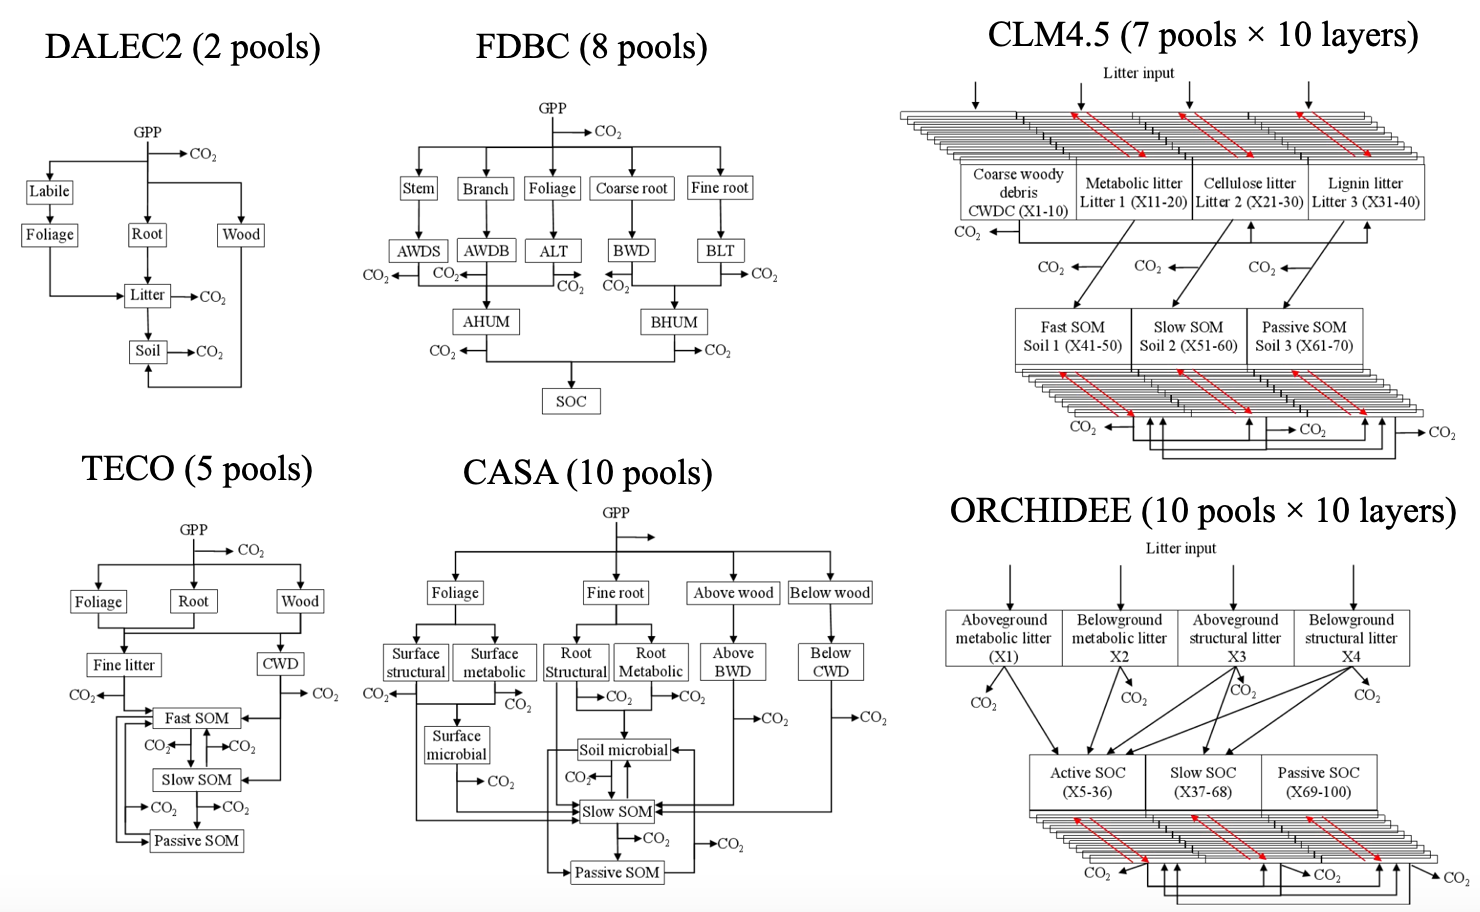
\includegraphics[width=15cm,height=15cm,keepaspectratio]{CLIMA-land/LM_figures/DOC_Diagrams_diff_complexity.png}
\caption{Schematic of decomposition model of different complexities. Litter and soil organic matter (SOM) in CLM and ORCHIDEE are vertically resolved, with 10 layers in each pool}
\label{f:Diagrams of soil organic carbon schemes of different complexities.}
\end{figure}


\subsection{Vertically resolved vs. total column formulations}

-Simplest formulation with no vertical dimension; more complex hypotheses with discrete vertical layers and continuous vertical dimension

-Do we include lateral movement (eg. runoff) of dissolved organic carbon (DOC) and dissolved inorganic carbon (DIC)? The C loss from runoff is on the same scale of $CH_4$ emission in a northern peatland.

\subsection{Environmental scalars}

\subsubsection{Temperature scalar}

-Q10 vs. alternative formulations

\subsubsection{Moisture scalar}
-High moisture suppression effect on aerobic respiration
-Joint aerobic and anaerobic respiration

\subsection{N limitation of decomposition fluxes}
\subsection{External N cycle}
\subsection{Methane model}
-one or multiple layers
-processes included 1)production only or 2)plus other processes (oxidation, emission pathways)

\section{Leaf Phenology}

The quantity of leaves within the canopy is computed based on the generic phenology model described in \citet{Knorr2010}. 

\subsection{A General Spatial Approach}

The typical approach to modeling leaf phenology is by using one or more growth triggers (or thresholds) that transition the vegetation into or out of an active growth state. This is problematic given that this is often modeled using a discrete formulation such as an if statement. In reality, plants over a given region (or grid cell) do not reach these thresholds simultaneously. There is likely to be a distribution of individual plants with individual triggers, resulting in a relatively smooth transition toward the new growth state. The model of \citet{Knorr2010} assumes that the "spatial variability within a grid cell is entirely the result of differences in the threshold parameter defining the trigger, effectively subsuming impacts of small‐scale climatic variability under the same". To model this, the threshold parameter is represented as a normal distribution in space. While this is a convenient solution to the problem, it is also grounded in the understanding that "dormancy in buds is not a single state, but rather a range of states that can vary within an individual over the course of the activity-dormancy cycle, between individuals of a species, and also between species" \citep{Cooke2012}. 

We can first consider a general formulation for the LAI of an individual plant ($\tilde{\Lambda}$) that switches into a growth phase when air temperature ($T$) exceeds that plants threshold temperature ($\tilde{T_{\phi}}$). When this condition is not met, the plant is not in an active growth phase. This can be represented by a differential equation in time ($t$) as follows:

\begin{equation}
\label{e:phenology_lai_discrete}
    \frac{d\tilde{\Lambda}(t)}{dt} = 
    \begin{cases}
    f_1,  &  \text{if }T \geq \tilde{T}_{\phi},\\
    f_2, &  \text{else, }
    \end{cases}
\end{equation}

where $f_1$ and $f_2$ are some arbitrary functions describing the state of the plant during the growth phase and senescent phase, respectively. This discrete formulation means that the relationship between LAI and the threshold parameter $\tilde{T}_{\phi}$ is non-differentiable at the transition point of the threshold. To overcome this, the spatially integrated LAI considers all individual plants within a grid cell, each with their own threshold parameter. Thus, the spatially integrated LAI ($\Lambda$) is represented by:

\begin{equation}
\label{e:phenology_lai_integral_temp}
    \frac{d\Lambda(t)}{dt} = f_1 \int_{-\infty}^{T} p(\tilde{T}_{\phi}) \; d\tilde{T}_{\phi} - f_2 \left( 1 - \int_{-\infty}^{T} p(\tilde{T}_{\phi}) \; d\tilde{T}_{\phi} \right)
\end{equation}

where $p$ is equal to a spatial Gaussian probability density function of the threshold variable $\tilde{T}_{\phi}$, with a mean $T_{\Phi}$ and standard deviation $T_r$. Additional threshold conditions can be included such as the day length ($t_d$). In the case of two threshold conditions (temperature and day length), the spatially integrated LAI is represented by:

\begin{equation}
\label{e:phenology_lai_integral_tempdaylength}
    \frac{d\Lambda(t)}{dt} = f_1 \int_{-\infty}^{T} \int_{-\infty}^{t_d} p(\tilde{T}_{\phi}) \; q(\tilde{t_{c}}) \; d\tilde{T}_{\phi} \; d\tilde{t_{c}} - f_2 \left( 1 - \int_{-\infty}^{T} \int_{-\infty}^{t_d} p(\tilde{T}_{\phi}) \; q(\tilde{t_{c}}) \; d\tilde{T}_{\phi} \; d\tilde{t_{c}} \right)
\end{equation}

where $q$ is equal to a spatial Gaussian probability density function of the threshold variable $\tilde{t_{c}}$, with a mean $t_{c}$ and standard deviation $t_r$. 

We can simplify this equation if we consider the integral as a cumulative distribution function ($\Phi$), again described by the deviation from the mean. This, again, is the cumulative distribution in space, not time. This results in the following: 

\begin{equation}
\label{e:phenology_lai_integral_simple}
    \frac{d\Lambda(t)}{dt} = f_1 f - f_2 (1 - f)
\end{equation}
with

\begin{empheq}[box=\eqnbox]{equation}\label{e:phenology_lai_cdf}
    f = \int_{-\infty}^{T} p(\tilde{T}_{\phi}) \; d\tilde{T}_{\phi} \; \int_{-\infty}^{t_d} q(\tilde{t_{c}}) \; d\tilde{t_{c}} \; = \; \Phi \left( \frac{T - T_{\phi}}{T_r} \right) \Phi \left( \frac{t_d - t_c}{t_r} \right),
\end{empheq}

alternatively, the temperature and day-length functions can be computed separately as follows: 

\begin{equation}
\label{e:phenology_lai_cdf_temp-daylength}
\begin{split}
    f(T) & = \Phi \left( \frac{T - T_{\phi}}{T_r} \right) \\
    f(t_d) & = \Phi \left( \frac{t_d - t_c}{t_r} \right)
\end{split}
\end{equation}

This represents the spatially integrated LAI response to threshold variables, $T$ and $t_d$, where $f$ varies between 0 and 1. Given that we're integrating over individual plants within a grid cell, the variable $f$ represents the fraction of plants in an active growth state. 

\subsection{Temporal Evolution of LAI}

With the general spatial approach described above we require some formulation for the evolution of the LAI of an individual plant over time. This requires a formulation for the two states of a plant, active growth ($f_1$) and a senescent state ($f_2$). \citet{Knorr2010} uses a relatively simple formulation for these two states and assumes the following: "leaf growth starts immediately and is not limited by substrate availability, such as LAI itself; and growth stops if a target LAI is reached that is in balance with the environmental limitations". This target LAI is given by $\Lambda_{max}$. Thus, the active growth function takes the form:

\begin{equation}
\label{e:phenology_lai_f1}
    f_1 = \xi (\Lambda_{max} - \Lambda)
\end{equation}

Where $\xi$ is a linear growth constant that describes the increase in LAI per unit time shortly after bud burst. This rate is assumed to be independent of the current NPP, as often the initial growth following bud burst is determined by the previous growing seasons carbon gains. 

For plants outside of their growth stage, a simplest possible formulation is the following:

\begin{equation}
\label{e:phenology_lai_f2}
    f_2 = \frac{\Lambda}{\tau_L}
\end{equation}

Where the parameter $\tau_L$ represents leaf longevity (in days) i.e. how quickly leaves are shed or whether they stay inactive until the next growing season. 

Combining these two growth state formulations with spatially integrated LAI as in Eq. \ref{e:phenology_lai_integral_simple}, we get

\begin{equation}
\label{e:phenology_lai_integral_f1f2}
    \frac{d\Lambda(t)}{dt} = \xi \big( \Lambda_{max} - \Lambda(t) \big) f - \frac{\Lambda(t)}{\tau_L} (1 - f)
\end{equation}

\citet{Knorr2010} goes further, simplifying this differential equation to provide a convenient form for integrating Eq. \ref{e:phenology_lai_integral_f1f2}. They define 

\begin{empheq}[box=\eqnbox]{equation}\label{e:phenology_lai_r}
    r = \xi f + \frac{(1 - f)}{\tau_L}
\end{empheq}

%\begin{equation}
%\label{e:phenology_lai_r}
%    \textcolor{blue}{ r = \xi f + \frac{(1 - f)}{\tau_L} }
%\end{equation}

and 

\begin{empheq}[box=\eqnbox]{equation}\label{e:phenology_lai_Lambda_lim}
    \Lambda_{lim} = \frac{\xi \Lambda_{max} f}{r}
\end{empheq}

%\begin{equation}
%\label{e:phenology_lai_Lambda_lim}
%    \textcolor{blue}{ \Lambda_{lim} = \frac{\xi \Lambda_{max} f}{r} }
%\end{equation}

In order to prevent $\Lambda_{lim}$ from going to to zero, it is kept positive by using an exponentially smoothed maximum of Eq. \ref{e:phenology_lai_Lambda_lim} and a small positive value, using

\begin{equation}
\label{e:phenology_lai_lambdalim_expsmoothed}
    \nu(x,y,x_0) = 
    \begin{cases}
        x + x_0 e^{-(x-y)/x_0-1},  &  \text{if } x \geq (y - x_0),\\
        y, &  \text{else, }
    \end{cases}
\end{equation}

where $\nu$ is the smoothed exponential maximum function, $x$ = $\Lambda_{lim}$ from Eq. \ref{e:phenology_lai_Lambda_lim}, $y$ = 1e-9, and $x_0$ = 5e-3. 

With the definition of $r$ and $\Lambda_{lim}$, Eq. \ref{e:phenology_lai_integral_f1f2} becomes:

\begin{equation}
\label{e:phenology_lai_final}
\begin{split}
    \frac{d\Lambda(t)}{dt} & = \xi \Lambda_{max} f - r \Lambda(t) \\
    & = r \big( \Lambda_{lim} - \Lambda(t) \big)
\end{split}
\end{equation}

With this, the term $r$ represents the inverse rate of growth ($days^{-1}$) and $\Lambda_{lim}$ represents the LAI limit of the current time-step to which $r$ approaches. 

The implementation of Eq. \ref{e:phenology_lai_final} within the model is done by updating the LAI incrementally. Thus, Eq. \ref{e:phenology_lai_final} has the solution:

\begin{empheq}[box=\eqnbox]{equation}\label{e:phenology_lai_incremental}
    \Lambda(t + \Delta t) = \Lambda_{lim} - \big( \Lambda_{lim} - \Lambda(t) \big) e^{-r \Delta t}
\end{empheq}

%\begin{equation}
%\label{e:phenology_lai_incremental}
%    \textcolor{blue}{ \Lambda(t + \Delta t) = \Lambda_{lim} - \big( \Lambda_{lim} - \Lambda(t) \big) e^{-r \Delta t} }
%\end{equation}

Where $\Delta t$ is the time step of the leaf phenology model, usually daily. 

\subsection{Temperature Limitations}

The model of \citet{Knorr2010} avoids the use of growing degree day sums which are typically used in models to simulate temperature requirements for growth of cold climate vegetation. Such a formulation has two pitfalls. First, these approaches typically yield a discrete transition into a growth phase, triggered when the growing degree days exceed a pre-defined critical value. This can lead to non-differentiable transitions. Second, many models that employ this approach must arbitrarily reset the accumulated growing degree days variable each winter or at the beginning of the calendar year (e.g. for northern hemisphere vegetation). \citet{Knorr2010} takes a slightly different approach using a smooth formulation to account for temperature and/or day length thresholds. 

For temperature, this approach applies exponentially declining weights to temperature going back in time, equivalent to an exponentially declining memory of a plant to temperature. To represent this, the phenology determining temperature $T$ is formulated as

\begin{equation}
\label{e:phenology_lai_temp}
\begin{split}
    T(t) & = \frac{ \int_{-\infty}^{0} T_{air} (t+\tilde{t}) e^{\tilde{t} / \tau_m} d \tilde{t} }{ \int_{-\infty}^{0} e^{\tilde{t} / \tau_m} d \tilde{t}}  \\
    & = \frac{1}{ \tau_m } \int_{-\infty}^{0} T_{air} (t + \tilde{t}) e^{\tilde{t} / \tau_m} d \tilde{t} \\
    & = \frac{1}{ \tau_m } e^{-t / \tau_m}  \int_{-\infty}^{0} T_{air} (t') e^{t' / \tau_m} d t'
\end{split}
\end{equation}

where $\tau_m$ is the period over which $T$ is averaged. A sensible value for $\tau_m$ is 30 days. 

Again, the implementation of this equation is simplified by bringing it into an incremental form:

\begin{equation}
\label{e:phenology_lai_temp_incremental}
\begin{split}
    T(t+\Delta t) & = \frac{1}{ \tau_m } e^{-(t+\Delta t) / \tau_m}  \int_{-\infty}^{(t+\Delta t)} T_{air} (t') e^{t' / \tau_m} d t'  \\
    & = \frac{1}{ \tau_m } e^{-\Delta t / \tau_m} e^{-t / \tau_m} \bigg( \int_{-\infty}^{t} T_{air} (t') e^{t'/ \tau_m} d t' + \int_{-\infty}^{t+\Delta t} T_{air} (t') e^{t'/ \tau_m} d t' \bigg) \\
    & = e^{-\Delta t / \tau_m} T(t) + \frac{1}{ \tau_m } e^{-(t+\Delta t) / \tau_m} \int_{t}^{t+\Delta t} T_{air} (t') e^{t'/ \tau_m} d t' \\
\end{split}
\end{equation}

If $\Delta t$ is the time step of the leaf phenology model (usually daily) and $T_{air}$ is constant over that period, this simplifies to:

\begin{empheq}[box=\eqnbox]{equation}\label{e:phenology_lai_temp_incremental2}
    T(t+\Delta t) = e^{-\Delta t / \tau_m} T(t) + T_{air}(t) ( 1 - e^{-\Delta t / \tau_m} )
\end{empheq}

%\begin{equation}
%\label{e:phenology_lai_temp_incremental2}
%    \textcolor{blue}{ T(t+\Delta t) = e^{-\Delta t / \tau_m} T(t) + T_{air}(t) ( 1 - e^{-\Delta t / \tau_m} ) }
%\end{equation}

This allows for $T$ to be updated at each model time step rather than computed using Eq. \ref{e:phenology_lai_temp} which requires accessing variables in past (i.e. $T_{air}$ over the past 30 days). 

\subsection{Water and Structural Limitations}

In the absence of well-defined mechanisms linking plant water status to LAI, \citet{Knorr2010} develops a simple approach to modeling a water-limited LAI ($\Lambda_W$). The principle is that "leaf development will stop and leaves will be shed if there is insufficient soil water for transpiration". The precise balance of plant available soil water and water required for transpiration may be a function of the adaptations of the plant e.g. life history and genetics. This adaptation is represented by a single parameter, $\tau_W$. This parameter defines the length of time a plant will tolerate water shortages before leaf shedding. In order to maintain a given LAI (the water-limited LAI; $\Lambda_W$), the amount of transpiration that can occur over a given time period must be balanced by the plant available soil moisture ($W$) as follows:

\begin{equation}
\label{e:phenology_lai_water_1}
    E(\Lambda_W) \tau_W = W
\end{equation}

To make use of this, we require a function for the potential water loss after time $\tau_W$ as a function of LAI. In \citet{Knorr2010}, they apply a linear relationship between LAI and the potential transpiration rate $E$ with

\begin{equation}
\label{e:phenology_lai_water_2}
    E(\Lambda) \approx \frac{\tilde{E}}{\tilde{\Lambda}} \Lambda
\end{equation}

where $\tilde{E}$ is the daily mean potential rate of transpiration last computed by the model at an LAI of $\tilde{\Lambda}$. This is, however, a simple approximation of how transpiration and LAI relate. \citet{Knorr2010} notes that this may only be valid for low LAI values where net radiation drives the evapotranspiration. A more appropriate form may include a saturating function. 

Combining Eq. \ref{e:phenology_lai_water_1} and \ref{e:phenology_lai_water_2} gives:

\begin{empheq}[box=\eqnbox]{equation}\label{e:phenology_lai_water_3}
    \Lambda_W = \frac{W \tilde{\Lambda}}{\tilde{E} \tau_W}
\end{empheq}

%\begin{equation}
%\label{e:phenology_lai_water_3}
%    \textcolor{blue}{ \Lambda_W = \frac{W \tilde{\Lambda}}{\tilde{E} \tau_W} }
%\end{equation}

Under a steady $W$, if $\tilde{E}$ declines then $\Lambda_W$ increases such that water-limitation becomes weaker on LAI. Similarly, if $W$ declines

If the ratio between $W$ and $\tilde{E} \tau_W$ decreases (e.g. $W$ is smaller than $\tilde{E} \tau_W$) then $\Lambda_W$ will decline i.e. LAI becomes more water-limited. In general, as $\tau_W \xrightarrow$0, $\Lambda_W \xrightarrow$ $\infty$ as the plant assumes water will always be available for leaf growth. Thus, vegetation without any water-driven leaf phenology will have $\tau_W=0$. 

Water limitation is not the only limiting factor in growth of new leaves, so an overall maximum potential LAI is introduced with the parameter $\hat{\Lambda}$. This represents the maximum LAI possible given other constraints such as physical structure, light, or nutrients. We take the actual LAI to be the minimum of the two potentially limiting LAI values, $\Lambda_W$ and $\hat{\Lambda}$, as follows:

\begin{empheq}[box=\eqnbox]{equation}\label{e:phenology_lai_waterstructure}
    \tilde{\Lambda}_{max} = \nu \left( \hat{\Lambda}, \Lambda_W \right)
\end{empheq}

%\begin{equation}
%\label{e:phenology_lai_waterstructure}
%    \textcolor{blue}{ \tilde{\Lambda}_{max} = \nu \left( \hat{\Lambda}, \Lambda_W \right) }
%\end{equation}

Where $\nu$ is a quadratic minimum function that provides a smooth transition between $\hat{\Lambda}$ and $\Lambda_W$, defined by

\begin{equation}
\label{e:phenology_lai_waterstructure_quadsmoothed}
    \nu(x,y) = \frac{x + y - \sqrt{(x+y)^2 - 4\eta x y}}{2 \eta}
\end{equation}

where $\eta$ is the degree of smoothing, typically $\eta$ = 0.9. 

The incorporation of $\tilde{\Lambda}_{max}$ from Eq. \ref{e:phenology_lai_waterstructure} into Eq. \ref{e:phenology_lai_Lambda_lim} is not direct. We do not compute $\tilde{\Lambda}_{max}$ using only instantaneous values for $W$ and $\tilde{E}$ but instead use a time weighted integration similar to that for temperature (in Eqs. \ref{e:phenology_lai_temp} and \ref{e:phenology_lai_temp_incremental2}). Hence,

\begin{equation}
\label{e:phenology_lai_waterstructure_quadsmoothed}
    \Lambda_{max}(t) = \frac{1}{ \tau_s } e^{-t / \tau_s}  \int_{-\infty}^{0} \tilde{\Lambda}_{max} (t') e^{t' / \tau_s} d t'
\end{equation}

and this can be updated incrementally (as is done for $T$ in Eq. \ref{e:phenology_lai_temp_incremental2}) as follows

\begin{empheq}[box=\eqnbox]{equation}\label{e:phenology_lai_waterstructure_incremental}
    \Lambda_{max}(t+\Delta t) = e^{-\Delta t / \tau_s} \Lambda_{max}(t) + \tilde{\Lambda}_{max}(t) ( 1 - e^{-\Delta t / \tau_s} )
\end{empheq}

%\begin{equation}
%\label{e:phenology_lai_waterstructure_incremental}
%    \textcolor{blue}{ \Lambda_{max}(t+\Delta t) = e^{-\Delta t / \tau_s} \Lambda_{max}(t) + \tilde{\Lambda}_{max}(t) ( 1 - e^{-\Delta t / \tau_s} ) }
%\end{equation}

where $\tau_s$ is the period over which $\Lambda_{max}$ is averaged ($\tau_s$ = 30 days). In practice, $\Lambda_{max}$ from Eq. \ref{e:phenology_lai_waterstructure_incremental} is substituted into Eq. \ref{e:phenology_lai_Lambda_lim}. 


\subsection{Light Intensity Controlled Leaf Dynamics}

The leaf phenology model of \citet{Knorr2010} presents hypotheses on the control of temperature, day length, and water availability on leaf growth and senescence. Measurements of leaf phenology in tropical forests suggest another potential control, light intensity. Some studies have highlighted the relationship between increasing light intensity and leaf litterfall in the Amazon at the beginning of the dry season \citep{}. Along transects in one part of the Amazon forest, \citet{Rice2004} found that litterfall was higher with lower precipitation, potentially suggesting a role of increasing light availability. 

While water availability is likely to impose limitations on leaf phenology, the availability of light is likely to drive changes in leaf phenology as well. \citet{Kim2012} introduced this mechanism into the Ecosystem Demography model 2 (ED2). The equations are given below. 

A quick but important side note here: We must take into consideration that the ED2 model approximates sub-grid variability in canopy structure and composition by using a system of size- and age-structured partial differential equations \citep{Medvigy2009}. This sub-grid variability is designed to "approximate the ensemble mean behavior of a corresponding individual‐based stochastic gap model" \citep{Medvigy2009} i.e. it approximates the population densities of individuals of each plant type and size class that make up the grid-scale canopy. Thus, in practice ED2 implements the two equations below per plant type, per plant size class, and per sub-grid tile. It is worth noting that \citet{Weng2015} developed a potentially more favourable approach that reduces the numerical complexity used in ED2, providing an analytically tractable set of equations for modeling the sub-grid scale variability, and included a competitively optimal carbon allocation scheme under the "perfect plasticity approximation" hypothesis \citet{Franklin2020}. 

The primary mechanism is the impact of radiation on the leaf turnover rate ($\alpha_{leaf}$). Each individual plant has the $\alpha_{leaf}$ computed by:

\begin{equation}
\label{e:phenology_leafturnover_radiation}
    \alpha_{leaf} = (\alpha_1 \bar{I} + \alpha_2) \alpha_0
\end{equation}

Further to this, \citet{Kim2012} introduced a relationship between leaf longevity ($\tau_L$ in BETHY, $LL$ in ED2), the inverse of $\alpha_{leaf}$, and the maximum potential carboxylation capacity ($V_{cmax}$). This is developed from knowledge of the coordination between leaf lifespan and photosynthetic capacity \citep{Wright2004}. This relationship is represented by a sigmoidal function as follows,

\begin{equation}
\label{e:phenology_leafturnover_vcmax_coord}
    V_m = \frac{V_m^{amp}}{\big( 1 + (\frac{LL}{LL^{trans}})^{V_m^{slope}} \big)} + V_m^{min}
\end{equation}

where the minimum $V_m$ is given by $V_m^{min}$, and the maximum $V_{m}$ is given by $V_m^{min}$+$V_m^{amp}$. The $V_m^{slope}$ is the rate at which $V_m$ changes with respect to $LL$. 

\subsection{Carbon Supply Limitation}

In principle the supply of carbon (NPP) can limit the growth of new leaves and thus have some control over leaf phenology. In its simplest terms, the amount of carbon allocated to new leaves can be represented by

\begin{equation}
\label{e:phenology_lai_water_1}
C_{leaf} = f_{leaf} \; NPP \; SLA
\end{equation}

where $f_{leaf}$ is the fraction of NPP allocated to leaf development and $SLA$ is the specific leaf area (the reciprocal of leaf mass per area). 


\subsection{Leaf Shedding and Litter Production}

The model of \citet{Knorr2010} also derives the mass of leaves that are shed and hence the amount of carbon that is contributed to the leaf litter. This is calculated as

\begin{empheq}[box=\eqnbox]{equation}\label{e:phenology_lai_shed}
    C_{leaf shed} (t) = C_{dm} \; \frac{ \nu \left( (\Lambda(t) - \Lambda_{lim}(t) ) (1 - e^{-r \Delta t)}, 0.0, 0.001 \right)}{SLA} 
\end{empheq}

%\begin{equation}
%\label{e:phenology_lai_shed}
%    C_{leaf shed} (t) = C_{dm} \; \frac{ \nu \left( \Lambda_{lim}(t) - \Lambda (t) (1 - e^{-\Delta t / r)}, 0.0, 0.001 \right)}{SLA} 
%\end{equation}

where $C_{dm}$ is the carbon content of dry matter ($g C \; g \; dry \; matter^{-1}$), SLA is the specific leaf area (the reciprocal of leaf mass per area), and $\nu$ is an exponential maximum function, equivalent to Eq. \ref{e:phenology_lai_lambdalim_expsmoothed}.



\begin{table}[]
\resizebox{\textwidth}{!}{%
\begin{tabular}{lllll}
State Variables         & Description                           & Units                     & Definition                            & Typical value     \\ \hline
 $\Lambda$                    & Leaf area index & m$^2$ m$^{-2}$ & Eq. \ref{e:phenology_lai_incremental} & $0\le \Lambda \le 12$ \\
   $T$                    & Leaf phenology temperature memory &  $^{\circ}$C & Eqs. \ref{e:phenology_lai_temp_incremental2}, \ref{e:phenology_lai_cdf_temp-daylength} & $0\le T \le 50$ \\
   $t_d$                    & Day-length &  hours & Eq. \ref{e:phenology_lai_cdf_temp-daylength} & $0\le t_d \le 24$ \\
   $W$                    & Plant available soil water & mm & Eq. xx & $0\le W \le xx$ \\
   $\tilde{E}$                    & Daily potential transpiration rate & mm day^{-1} & Eq. xx & $1e-3\le \tilde{E} \le xx$ \\  [2ex]
Functions of State      & Description                           & Units                     & Definition                            & Typical value \\ \hline
    $f$                    & Fraction of plants in active growth state & - & Eqs. \ref{e:phenology_lai_cdf}, \ref{e:phenology_lai_cdf_temp-daylength} & $0\le f \le 1$  \\
    $f_1$                    & Active growth function & LAI day$^{-1}$ & Eq. \ref{e:phenology_lai_f1} & -  \\
    $f_2$                    & Senescent phase function & LAI day$^{-1}$ & Eq. \ref{e:phenology_lai_f2} & -  \\  
    $\Lambda_{max}$                    & Maximum leaf area index & m$^2$ m$^{-2}$ & Eq. xx & $0\le t_d \le 12$ \\
   $\Lambda_{lim}$                    & Leaf area index limit & m$^2$ m$^{-2}$ & Eq. xx & $1e-9\le t_d \le 12$ \\
   $\Lambda_W$                    & Water-limited leaf area index & m$^2$ m$^{-2}$ & Eq. xx & $1e-9\le \Lambda_W \le 12$ \\
   $r$                    & Inverse growth rate & days$^{-1}$ & Eq. xx & $0\le r \le 1$ \\  [2ex]
Empirical Properties      & Description                           & Units                     & Definition                            & Typical value \\ \hline
$T_{\phi}$             & Mean temperature at leaf onset       & $^{\circ}$C   & Eq. xx     & $-\infty\le T_{\phi} \le 50$   \\
$T_r$             & Spatial range (1$\sigma$) of $T_{\phi}$       & $^{\circ}$C   & Eq. xx     & $0.5\le T_{r} \le 15$   \\
$\tau_m$             & Time interval over which $T$ is averaged       & days   & Eq. \ref{e:phenology_lai_temp_incremental2}     & 30   \\
$t_c$             & Mean day length at leaf shedding       & hours   & Eq. xx     & $0\le t_c \le 24$   \\
$t_r$             & Spatial range (1$\sigma$) of $t_c$       & hours   & Eq. xx     & $0.5\le t_{r} \le 24$   \\
$\hat{\Lambda}$             & Physical maximum leaf area index       & m$^2$ m$^{-2}$   & Eq. xx     & $0.05\le \hat{\Lambda} \le 12$   \\
$\xi$             & Initial linear leaf growth rate      & days$^{-1}$   & Eq. xx     & $0.01\le \xi \le 50$   \\
$k_L$             & Inverse leaf longevity ($\tau_L$)      & days$^{-1}$   & Eq. xx     & $1e-3\le k_L \le 0.2$   \\
$\tau_W$             & Target survival time under water-deficit conditions      & days   & Eq. \ref{e:phenology_lai_water_3}     & $0\le \tau_W \le 365$   \\
$\tau_s$             & Time interval over which $\Lambda_{max}$ is averaged  & days   & Eq. \ref{e:phenology_lai_waterstructure_incremental}     & 30   \\

%\hline
\end{tabular}%
}% end resizebox
\caption{\label{t:leaf_phenology_variables}Key leaf phenology variables and parameters. See \citet{Knorr2010} and \citet{Kim2012} for further details.}
\end{table}

\end{document}








\section{Stuff from Previous Version}

In the soil, heat follows a 1D vertical heat diffusion:
\begin{equation}
     \frac{\partial (C_s T_s) }{\partial t} = \frac{\partial }{\partial z}\kappa \frac{\partial T_s }{\partial z} + S_T
\end{equation}
where $C_s$--the volumetric heat capacity--is the product of soil density and specific heat capacity, i.e.  $C_s = \rho_s c_s$, and are defined in subsequent sections, and $\kappa$ is the thermal conductivity of the soil, $S_T$ are sources of heat such as phase change. Phase change heating rate can be expressed as: 
\begin{equation}
    S_T = \rho L_m \frac{\partial \theta_{ice}}{\partial t}_{|{\rm ice-liquid \ change}}.
    \end{equation}
with $\frac{\partial \theta_{ice}}{\partial t}_{|{\rm ice-liquid \ change}}$ the local rate of change of liquid into ice. 


We can combine the phase change with temperature defining a total energy $H=C_s T_s+ \rho L_m \theta_{ice}$ and an ice-conserved temperature $T_{\rm ice}=H/C_s$ to get:
\begin{equation}
     \frac{\partial H }{\partial t}  =  \frac{\partial }{\partial z}\kappa \frac{\partial T_s }{\partial z}
\end{equation}
or using $T_{\rm ice}$:
\begin{equation}
     \frac{\partial (C_s T_{\rm ice})}{\partial t} =  \frac{\partial }{\partial z}\kappa \frac{\partial T_s }{\partial z}
\end{equation}

\begin{figure}[htb]
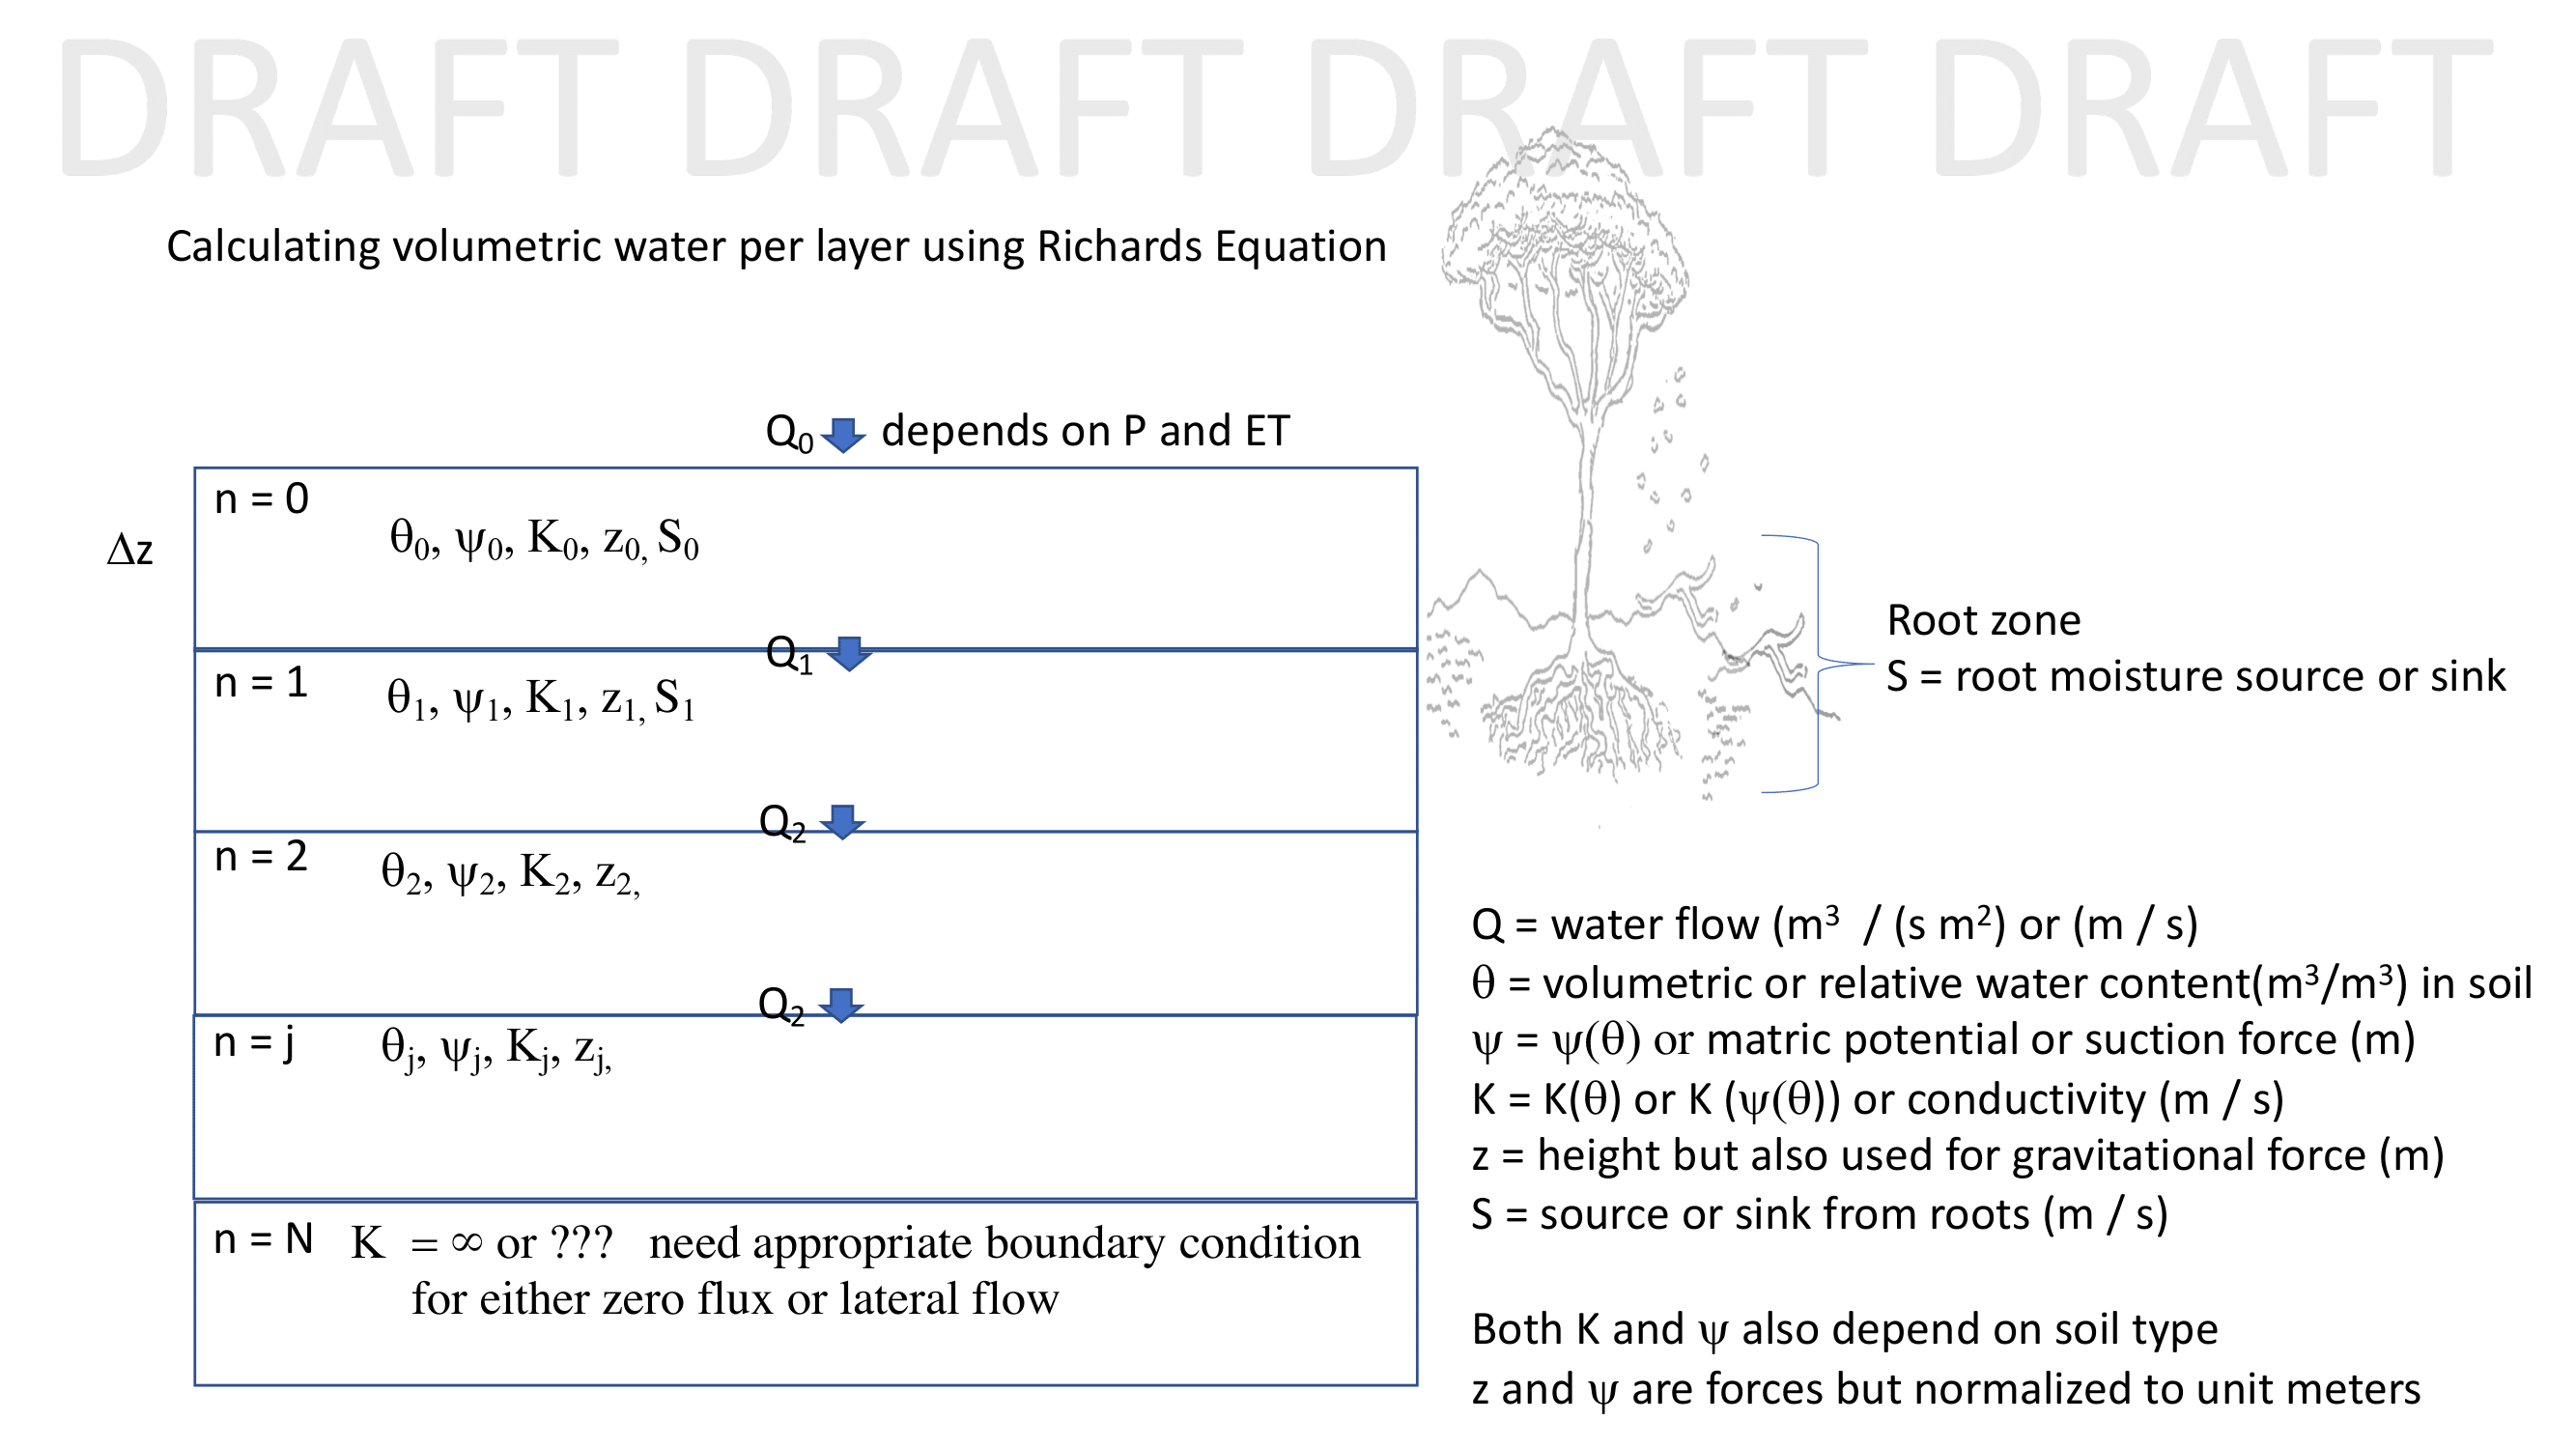
\includegraphics[scale=.15]{CLIMA-land/LM_figures/SoilSchematic-1.png}
\caption{Draft of soil schematic figure}
\end{figure}


\subsection{Phase Change}

The freezing of soil water or melting of soil ice releases or absorbs energy, respectively. Formation of ice releases latent heat, and temperature remains constant at the freezing point while soil water freezes. Similarly, melting of ice consumes energy, during which temperature does not increase. Latent heat of fusion is the amount of energy required to convert a unit of mass of frozen water to liquid. This transition requires 334 J g$^{-1}$. Freezing liquid water to ice releases a similar amount of energy. The total energy involved in phase change depends on soil moisture. For a volumetric water content $\theta$, the energy (J m$^{-3}$) required to freeze soil is $L_f \rho_{wat} \theta$, where $L_f =$ 0.334 MJ kg$^{-1}$ is the latent heat of fusion of water and $\rho_{wat} =$ 1000 kg m$^{-3}$ is the density of water. In course-grained soil such as sands, all the water present in the soil changes phase at a temperature close to 0$^{\circ}$C ($T_f =$ 273.15 K).  These soils can be treated with good approximation as either completely frozen or unfrozen. In fine-grain soils such as silts and clays, some soil water remains unfrozen even at temperatures below freezing. The amount of unfrozen water decreases as temperature decreases, and the latent heat release occurs over some temperature range $T_f - \Delta T_f$.

A simple way to account for freezing and thawing is to add the latent heat associated with phase change to the heat conduction equation to yield an apparent heat capacity \citep{lunardini1981heat}. Including a latent heat term as the unfrozen water $\theta_{liq}$ freezes, the heat conduction equation becomes
\begin{equation}
     c_v \frac{\partial T}{\partial t} = \frac{\partial }{\partial z} \left( \kappa \frac{\partial T}{\partial z} \right) - L_f \rho_{wat} \frac{\partial \theta_{liq}}{\partial t}.
\end{equation}
The second term on the right-hand side of the equation is a source of energy during freezing ($\partial \theta_{liq} / \partial t <$ 0) and is a sink of energy during melting ($\partial \theta_{liq} / \partial t >$ 0). The change in liquid water can be expressed as $\partial \theta_{liq} / \partial t = ( \partial \theta_{liq} / \partial T) (\partial T / \partial t)$, and the equation above can be re-written as 
\begin{equation}
     \left( c_v\ +\ L_f \rho_{wat} \frac{\partial \theta_{liq}}{\partial T} \right)  \frac{\partial T}{\partial t} = \frac{\partial }{\partial z} \left( \kappa \frac{\partial T}{\partial z} \right).
\end{equation}
Written this way, the term in parentheses on the left-hand side of the equation represents an effective heat capacity. Solution of this equation requires an expression for $\partial \theta_{liq}/{\partial T}$ to relate the amount of liquid water to temperature. In practice, however, the entire latent heat of fusion can be associated with a small finite temperature range between the freezing point and $T_f -\Delta T_f$ so that the effective heat capacity for a soil with water content $\theta$ is
\begin{equation}
c_v = \left\{
        \begin{array}{lll}
            c_{vu} & \quad T\ >\ T_f, \\
            c_{vf}\ + \frac{L_f \rho_{wat} \theta }{\Delta T_f} & \quad T_f - \Delta T_f\  \leq  T\ \leq\ T_f\ ,\\
            c_{vf} & \quad  T\ \leq\ T_f - \Delta T_f\\
        \end{array}
    \right.
\end{equation}
where $c_{vu}$ and $c_{vf}$ are the unfrozen and frozen volumetric heat capacity, respectively. The apparent heat capacity is the heat capacity of soil constituents plus a term that accounts for the latent heat of fusion. 

\begin{comment}

\hl{[The following is covered in Eq. (2.6) above.]} The heat capacity of air is negligible so that the heat capacity of soil is given by the weighted fraction of the heat capacity of solids, water and ice \citep{de1963thermal}, and
\begin{equation}
c_v = (1- \theta_{sat}) c_{v,sol} +  \theta_{liq} c_{v,wat} +  \theta_{ice} c_{v,ice}.
\end{equation}
The heat capacity of water is $c_{v,wat}= \rho_{wat}c_{wat} =$ 4.19 MJ m$^{-3}$ K$^{-1}$, for ice $c_{v,ice}= \rho_{ice}c_{ice} =$ 1.94 MJ m$^{-3}$ K$^{-1}$, and for soil solids $c_{v,sol} =$ 1.926 MJ m$^{-3}$ K$^{-1}$ \citep{de1963thermal}. The equation above can be applied assuming all water is either liquid or ice to calculate the unfrozen and frozen heat capacity, respectively.  

\end{comment}

Using the chain rule of differentiation and the fact that the matric potential is a monotonic function of $\theta_l$, Darcy's law can also be written as
\begin{equation}\label{e:darcy_law2}
    \vec{\tilde d}_l = - K(\theta_l) \left(C_l(\theta_l)^{-1} \grad\theta_l + \grad \psi_z \right),
\end{equation}
where
\begin{equation}
C_l(\theta_l) = \left( \frac{d\psi}{d\theta_l} \right)^{-1} =   \frac{d\theta_l}{d\psi} 
\end{equation}
is known as the specific moisture capacity ($\mathrm{m^{-1}}$). The last equality is the derivative of the inverse $\theta_l(\psi)$ of the function $\psi(\theta_l)$, which is commonly used in hydrology and is known as the water retention curve. The quantity $K(\vec{\theta})/C(\vec{\theta})$ has units of diffusivity ($\mathrm{m^2~s^{-1}}$) is known as the soil water diffusivity. It is singular where the specific moisture capacity $C(\theta_l)$ is zero, which is the case in saturated soil. 

Integrating the water balance equation \eqref{e:soil_water_conservation} numerically is challenging primarily because of this singularity at the water table, where the unsaturated (vadose) zone meets the saturated zone \citep{Farthing17a}.

\subsection{Summary of soil heat and moisture equations for CliMA implementation}

This section contains a summary of all equations needed for implementation of the soil heat and moisture equations into CliMA. All variables are defined 

[OPTION: list equations in table for succinct description and avoid extra equation numbers in document] \\

\textbf{Soil Heat Equation} \\


\begin{equation}
     \frac{\partial (\rho_s c_s T_s) }{\partial t} = \frac{\partial }{\partial z}\kappa \frac{\partial T_s }{\partial z}
\end{equation}

\begin{equation}
    f_{\mathrm{om}} = \rho_{\mathrm{om}}/\rho_{om,{\rm max}}
\end{equation}


\begin{equation}
\kappa = K_e \kappa_{\rm sat} + (1-K_e) \kappa_{\mathrm{dry}}
\end{equation}

\begin{equation}
K_e = \exp \big( \gamma((1-s(\gamma-1.33))\big)
\end{equation}

\begin{equation}
s=\theta/\theta_{\rm sat}
\end{equation}

\begin{equation}
c_s=\theta c_{\rm liq} + (1-\theta) c_{\rm dry}
\end{equation}

\begin{equation}
c_{\rm dry} = (1-f_{\mathrm{om}})c_{soil} + f_{\mathrm{om}}c_{\mathrm{om}}
\end{equation}

\begin{equation}
c_{soil} = {\rm \frac{2.128 (sand)+ 2.385 (clay)}{(sand) + (clay)}}
\end{equation}  \\



\textbf{Soil Moisture Equations} \\

(Unsaturated soil)
\begin{equation}
 dS=d\theta 
\end{equation}

(Saturated - Unconfined Aquifer)
\begin{equation}
 dS=S_y dh ; S_y = n
\end{equation}

(Saturated - Confined Aquifer)
\begin{equation}
 dS=S_s dh
\end{equation}

\begin{equation}
 h=z+\psi
\end{equation}

\begin{equation}
dS = C(\psi)d\psi
\end{equation}

(Unsaturated soil)
\begin{equation}
C(\psi)=\partial \theta /\partial h 
\end{equation}

(Unconfined aquifer)
\begin{equation}
C(\psi)=S_y 
\end{equation}

(Richards' equation)
\begin{equation}
     \frac{\partial S}{\partial t} = C(\psi)\frac{\partial \psi}{\partial t} = -\nabla \cdot {\bf{q}} + {\rm Source}
\label{Richards}
\end{equation}

\begin{equation}
     \bf{q} = - \mathbf{K}(\psi) \otimes \nabla h
\end{equation}

(Unsaturated zone)
\begin{equation}
     \frac{\partial \theta}{\partial \psi}\frac{\partial h}{\partial t} = \frac{\partial}{\partial z} \left( {K(\psi)\frac{\partial \psi}{\partial z}} + 1 \right) + {\rm Source}
\end{equation} \\

(Saturated - Unconfined Aquifer)
\begin{equation}
     \frac{\partial S}{\partial t} = S_y \frac{\partial h}{\partial t} = \nabla \cdot \left( {K_{\rm sat} \nabla h} \right) + {\rm Source}
\end{equation} \\


\textbf{Retention functions for unsaturated soils - van Genuchten} \\


\begin{equation}
     \theta(\psi) = \theta_{\mathrm{res}} + \frac{\theta_{\mathrm{sat}} - \theta_{\mathrm{res}}}{\left[ 1+(\alpha |\psi|)^n \right]^{m}}
\end{equation}

\begin{equation}
m=1-1/n
\end{equation}

\begin{equation}
     K(\psi) = K_{\mathrm{sat}} S_l^L \left (1 -  (1-S_l^{1/m})^m  \right)^2
\end{equation}

\begin{equation}
L = 0.5
\end{equation}

\begin{equation}
     S_l = \frac{\theta(\psi) - \theta_{\mathrm{res}}}{\theta_{\mathrm{sat}} - \theta_{\mathrm{res}}}
\end{equation}

\begin{equation}
     \frac{\partial \theta}{\partial \psi} =   \frac{m n\alpha^n |\psi|^{n-1}}{\left[ 1+(\alpha |\psi|)^n \right]^{m+1}} \left( \theta_{\mathrm{sat}} - \theta_{\mathrm{res}} \right) 
\end{equation}


\subsubsection{Retention curves $\theta=f(\psi)$ and $K(\psi)$ in the unsaturated zone}
\label{SoilMoisture:Retention_Curves}
    {\bf Van Genuchten} \\
We will use the van Genuchten formulation as a reference retenstion curve, as it is better behaved in saturated conditions than the Brooks and Corey relationship 
\begin{equation}
     \theta(\psi) = \theta_{\mathrm{res}} + \frac{\theta_{\mathrm{sat}} - \theta_{\mathrm{res}}}{\left[ 1+(\alpha |\psi|)^n \right]^{m}}
\end{equation}
with $m=1-1/n$.
For hydraulic conductivity, we have
\begin{equation}
     K(\psi) = K_{\mathrm{sat}} S_l^L \left (1 -  (1-S_l^{1/m})^m  \right)^2
\end{equation}
with $L$ an empirical parameter assumed to be $L=0.5$. $S_l$ is the relative degree of saturation of the soil and $K_{\mathrm{sat}}$ the hydraulic conductivity at saturation. 
\begin{equation}
     S_l = \frac{\theta(\psi) - \theta_{\mathrm{res}}}{\theta_{\mathrm{sat}} - \theta_{\mathrm{res}}}
\end{equation}
The derivative of $\theta$ with respect to $\psi$, $C(\psi)$ is:
\begin{equation}
     \frac{\partial \theta}{\partial \psi} =   \frac{m n\alpha^n |\psi|^{n-1}}{\left[ 1+(\alpha |\psi|)^n \right]^{m+1}} \left( \theta_{\mathrm{sat}} - \theta_{\mathrm{res}} \right). 
\end{equation}


    {\bf Brooks and Corey} \\
An alternative approach to Van Genuchten will be to use the Brooks-Corey relationships:
\begin{equation}
     \theta(\psi) = \theta_{\mathrm{res}} + (\theta_{\mathrm{sat}} - \theta_{\mathrm{res}})\left( \frac{\psi}{\psi_{ae}}\right)^{-\lambda}
\end{equation}
with $\psi_{ae}$ the air entry point.
\begin{equation}
     K(\psi) = K_{\mathrm{sat}} \left( \frac{\psi}{\psi_{ae}}\right)^{-2-3\lambda}
\end{equation}


% Calculation of Kersten number and kappa_s for Thermal Conductivity calculation 
\begin{comment}
For unfrozen soil: \hl{[what is this based on? does it have a strong basis in global data?]}
\begin{equation}
K_e = \left\{
        \begin{array}{ll}
            1.0 + 0.7\ \mathrm{log_{10}}\ S_l & \mathrm{course-texture\ soil\ } (S_l > 0.05), \\
            1.0 + \mathrm{log_{10}}\ S_l & \mathrm{fine-texture\ soil\ } (S_l > 0.10)
        \end{array}
    \right.
\end{equation}
and fine-texture soil has a sand content of less than 50\%. For frozen soil:
\begin{equation}
K_e = S_l.
\end{equation}
In these equations, $S_l= \frac{\theta}{\nu_p}$ is the relative wetness, with $\theta$ as the volumetric water content (m$^{3}$ H20 m$^{-3}$ soil) and $\nu_p=\theta_{sat}$ as the volumetric water content at saturation (also equal to porosity). 

The dry and saturated thermal conductivities depend on soil properties. The thermal conductivity of dry soils varies with bulk density (kg m$^{-3}$) according to 
\begin{equation}
\kappa_{\mathrm{dry}} = \frac{ (0.135 \rho_\mathrm{b} + 64.7 )}{ (2700 - 0.947 \rho_\mathrm{b} )}.
\end{equation}
where $\rho_\mathrm{b} = 2700(1- \theta_{sat})$ and 2700 kg m$^{-3}$ here represents the density of soil solids. The thermal conductivity of saturated soil is calculated from the thermal conductivity of the components (solids $\kappa_{solids}$, water $\kappa_{liquid}$, and ice $\kappa_{ice}$) and their respective volume fractions. For unfrozen soil:
\begin{equation}\label{e:conductivity_sat}
\kappa_{\mathrm{sat}} = \kappa_{solids}^{(1- \theta_{sat} )}  \kappa_{liquid}^{(\theta_{sat} )}. 
\end{equation}
And for frozen soil:
\begin{equation}
\kappa_{\mathrm{sat}} = \kappa_{solids}^{(1- \theta_{sat} )}  \kappa_{ice}^{(\theta_{sat} )}. 
\end{equation}
A general expression allowing a mixture of liquid water and ice is
\begin{equation}
\kappa_{\mathrm{sat}} = \kappa_{solids}^{(1- \theta_{sat} )}  \kappa_{liquid}^{(f_u \theta_{sat} )}  \kappa_{ice}^{( (1-f_u) \theta_{sat} )}.
\end{equation}
This equation recognizes that even at temperatures below freezing, the total water consists of unfrozen $\theta_{liq}$ and frozen $\theta_{ice}$ water ($\theta = \theta_{liq} + \theta_{liq}$), and $f_u = \frac{\theta_{liq}}{\theta}$ is the fraction of the total water that is unfrozen. Representative values are $\kappa_{liquid} = 0.57$ W m$^{-1}$ K$^{-1}$ and $\kappa_{ice} = 2.29$ W m$^{-1}$ K$^{-1}$. 
The thermal conductivity of a soil varies with the quartz content of the soil. The Johansen method described by \citep{Farouki81a} gives an approximation of such a dependence on quartz content:
\begin{equation}
\kappa_{solids} = \kappa_{q}^q \kappa_{o}^{1-q},
\end{equation}
where $q$ is the quartz content as a fraction of the total soil solids, $\kappa_{q}$ = 7.7 W m$^{-1}$ K$^{-1}$ is the thermal conductivity of quartz, and $\kappa_{o}$ = 2.0 W m$^{-1}$ K$^{-1}$ is the thermal conductivity of other minerals for soils with $q >$ 0.2 and  $\kappa_{o}$ = 3.0 W m$^{-1}$ K$^{-1}$ for $q <=$ 0.2. The accuracy of this equation depends on the specified thermal conductivity of quartz and the quartz fraction. The quartz content can be approximated by the sand content (i.e. quartz fraction $q$ $\sim$= fraction of soil that is sand)  \citep{peters1998effect}, though this is not necessarily correct \citep{lu2007improved}.  
\end{comment}


% Old Explanation of Calculation of Kersten number and kappa_s for Thermal Conductivity calculation
\begin{comment}
The thermal conductivity of soil depends on the water content and is modeled as a weighted mean of a conductivity $\kappa_{\mathrm{dry}}$ of dry soil and a conductivity $\kappa_{\rm sat}$ of water-saturated soil,
\begin{equation}\label{e:soil_conductivity}
\kappa = K_e \kappa_{\mathrm{sat}} + (1-K_e) \kappa_{\mathrm{dry}}.
\end{equation}
The weighting factor $K_e$ is the Kersten number, which is function of soil relative humidity $s=\theta/\theta_{\rm sat}$. (However, the thermal diffusivity $\kappa/\tilde c_s$ has a much weaker moisture dependence than $\kappa$ itself because of a compensation of the moisture dependence between $\kappa$ and $\tilde c_s$.)

The saturation heat conductivity, even in the presence of frozen ground, can be expressed as a function of the ice and liquid water contents assuming a geometric mean: \hl{[why do we average geometrically here and arithmetically above? Seems odd.]}
\begin{equation}\label{e:conductivity_sat}
\kappa_{\mathrm{sat}} = \kappa_{solids}^{(1- \theta_{sat} )}  \kappa_{liquid}^{(f_u \theta_{sat} )}  \kappa_{ice}^{( (1-f_u) \theta_{sat} )} 
\end{equation}
where $\kappa_{\mathrm{sat}}$ is the thermal conductivity of a saturated soil, and is calculated from the thermal conductivity of the components ($\kappa_{solids}$, $\kappa_{liquid}$, and $\kappa_{ice}$), $\theta_{sat}$ is the volumetric water content at saturation (also equal to porosity), and $f_u = \theta_{liquid} / \theta$ is the fraction of total water that is unfrozen. Representative values are $\kappa_{liquid} = 0.57$ W m$^{-1}$ K$^{-1}$ and $\kappa_{ice} = 2.29$ W m$^{-1}$ K$^{-1}$. 
The thermal conductivity of a soil varies with the quartz content of the soil. The Johansen method described by \cite{Farouki81a} gives an approximation of such a dependence on quartz content:
\begin{equation}
\kappa_{solids} = \kappa_{q}^q \kappa_{o}^{1-q}
\end{equation},
where $q$ is the quartz content as a fraction of the total soil solids, $\kappa_{q}$ = 7.7 W m$^{-1}$ K$^{-1}$ is the thermal conductivity of quartz, and $\kappa_{o}$ = 2.0 W m$^{-1}$ K$^{-1}$ is the thermal conductivity of other minerals for soils with $q >$ 0.2 and  $\kappa_{o}$ = 3.0 W m$^{-1}$ K$^{-1}$ for $q <=$ 0.2.
\end{comment}


\subsection{Moisture equation - an alternative approach}

We note that there is a fundamental issue in the continuity of the Richards' equation at the water table interface. Indeed, $C(\psi)$ goes to zero at the bottom of the unsaturated zone but is a fixed value in the saturated zone (the specific yield), leading to sharp derivative discontinuity. We note that the specific yield is empirical, mainly based on measurements and is close to the soil moisture content at saturation $\theta_{\mathrm{sat}}$. We will return to this.

We write the porous medium temporal mass $M$ balance per unit volume as a departure from the hydrostatic pressure, equivalent to $\partial h/\partial z=0$, with $h=z+\psi$. The temporal departure from hydrostatic balance is written as $\psi'$ with corresponding changes in density $\rho'=\rho-\overline\rho$. The water porous medium density conservation reads:
\begin{equation}
\frac{\partial \rho \theta}{\partial t} = {\overline{\rho}} \nabla \cdot \left( K(\psi) \left( \nabla \psi + {\mathbf e_z} \right) \right)
\end{equation}
In which we have neglected the mass of water vapor.
We expand this into:
\begin{equation}
{\overline \rho} \frac{\partial \theta}{\partial t} + \theta \frac{\partial \rho}{\partial t} = {\overline \rho} \nabla \cdot \left( K(\psi) \left( \nabla \psi + {\mathbf e_z} \right) \right)
\end{equation}
Dividing by $\overline \rho$ gives:
\begin{equation}
\frac{\partial \theta}{\partial t} + \frac{\theta}{\overline \rho} \frac{\partial \rho}{\partial t} = \nabla \cdot \left( K(\psi) \left( \nabla \psi + {\mathbf e_z} \right) \right)
\end{equation}
This equation looks like the unsaturated Richards’ equation beside the presence of the second term on the left hand side, related to the compressibility of liquid water: $ \frac{\theta}{\overline \rho} \frac{\partial \rho}{\partial t}$.

We now use chain’s rule with respect to variations in internal pressure $\psi$ but do not assume that liquid water is incompressible, to write the mass change:
\begin{equation}
{\overline \rho} \frac{\partial \theta}{\partial t} + \theta \frac{\partial \rho}{\partial t} 
\end{equation}

In the unsaturated zone the second term on the lhs is negligible. In the saturated zone, the converse is true and the density term becomes important. At the water table interface, the $\theta=\theta_{\mathrm{sat}}=n$, the porosity assumed to be the same as the saturation water content $\theta_{s}$. We therefore further write $\theta$ in terms of the relative saturation content $s=\theta/\theta_{\mathrm{sat}}$.
The liquid water mass balance can be written
\begin{equation}
\underbrace{{\overline \rho} n \frac{\partial s}{\partial t} }_\text{\rm unsaturated mass change} + \underbrace{{\overline \rho} s \frac{\partial n}{\partial t}  }_\text{\rm change in porous medium porosity}  
+ 
\underbrace{\theta \frac{\partial \rho}{\partial t}   }_\text{\rm change in liquid water density}  
\label{mass_balance:split}
\end{equation}
The change in density (assuming negligible temperature and solute impact) can be written:
\begin{equation}
\frac{\partial \rho}{\partial t} = \rho \beta \frac{\partial \psi}{\partial t}
\end{equation}
with $\psi$ the pressure.
Assumed an elastic material (and neglecting the change in density of the material) (Bear 2018) and introducing the coefficient of porous medium compressibility $\alpha_{pm}$, with assumed veritcal stress:
\begin{equation}
\alpha_{pm}=\frac{1}{V_{pm}} \frac{\partial V_{pm}}{\partial \sigma_z} = \frac{1}{1-n} \frac{\partial n}{\partial \psi}
\end{equation}
with $\sigma_z$ the stress tensor in the vertical direction.
This then lead to the change in porosity due to the porous medium compaction:
\begin{equation}
\frac{\partial n}{\partial t} = (1-n)\alpha_{pm}\frac{\partial \psi}{ \partial \psi}
\end{equation}
The combined change in mass of the porous medium water can be finally written using equation (\ref{mass_balance:split}) 
\begin{equation}
\frac{\partial \theta \rho}{\partial t} = 
\underbrace{n \rho \frac{\partial s}{ \partial t} }_\text{\rm unsaturated mass change} + \underbrace{s \rho \left[  (1-n)\alpha_{pm} + n\beta \right] \frac{\partial \psi}{\partial t} }_\text{\rm saturated mass change}
\end{equation}
We note here that we made a convenient approximation: we used the matric potential $\psi$, instead of the pressure $p$. The rational for that is that far away from the water table the unsaturated term the left hand side domaintes. Within the saturated zone, far from the water table, the lhs vanishes. Yet an advantage is that the equation bcomes continuous at the interface, with continuous and non-vanishing temporal derivatives. Another way to think about this is that the fluid is composed of a mixture of saturated and saturated water at the interface - i.e the interface is not abrupt. 
Our master equation for the porous medium water conservation then becomes:
\begin{equation}
 \left( n \rho \frac{\partial s}{\partial \psi} + s \rho   (1-n)\alpha_{pm} + s n\beta \right) \frac{\partial \psi}{\partial t} = \rho \nabla \cdot \left( K(\psi) \left( \nabla \psi + {\mathbf e_z} \right) \right)
\label{master_equation_porous_medium}
\end{equation}
or dividing by $\rho$
\begin{equation}
\red{ n \left(  \frac{\partial s}{\partial \psi} + s \frac{1-n}{n}\alpha_{pm} + s \beta \right) \frac{\partial \psi}{\partial t} = \nabla \cdot \left( K(\psi) \left( \nabla \psi + {\mathbf e_z} \right) \right)}
\label{master_equation_porous_medium} 
\end{equation}







We now integrate the mass balance equation over the depth of the unconfined aquifer i.e. from $z=z_0$ to $z=h+\epsilon$ (with $z=z_0$ the bedrock elevation – not necessarily 0):
\begin{equation}
\int_{z_0}^{h+\epsilon} { n \left(  \frac{\partial s}{\partial \psi} + s \frac{1-n}{n}\alpha_{pm} + s \beta \right) \frac{\partial \psi}{\partial t}  dz = \int_{z_0}^{h+\epsilon} \nabla \cdot \left( K(\psi) \left( \nabla \psi + {\mathbf e_z} \right) \right)} dz
\end{equation}
\begin{equation}
\int_{z_0}^{h+\epsilon} { n \left(  \frac{\partial s}{\partial \psi} + s \frac{1-n}{n}\alpha_{pm} + s \beta \right) \frac{\partial \psi}{\partial t}  dz =
K(\psi) \left( \frac{\partial \psi}{\partial z} + 1 \right)_{|z=h+\epsilon} + \nabla_H \cdot \int_{z_0}^{h+\epsilon}  K(\psi) \nabla_H \psi dz
\end{equation}
Using Leibniz rule, the lhs can be written as 
\begin{equation}
\frac{\partial \int_{z_0}^h \rho \theta_{\mathrm{sat}} dz }{\partial t} - \rho \theta_{\mathrm{sat}} \frac{\partial h}{\partial t}=
K(\psi) \left( \frac{\partial \psi}{\partial z} + 1 \right)_{|z=h+\epsilon} \\
+ \nabla_H \cdot \int_{z_0}^{h+\epsilon}  K(\psi) \nabla_H \psi dz
\end{equation}
The rhs can be rewritten as:
\begin{equation}
\int_{z_0}^h  \nabla \cdot \left( {\overline \rho} K(\psi) \left(\nabla \psi + {\mathbf e_z} \right) \right) dz = {\overline \rho} K(\psi) \left(\nabla \psi + {\mathbf e_z} \right)_{|h}  + \int_{z_0}^h  \nabla_H \left( {\overline \rho} K(\psi) \left(\nabla_H \psi \right) \right) dz
\end{equation}

Because the rate of change of the water table is much larger than the changes in density, we have: 
\begin{equation}
-	\theta_{\mathrm{sat}} \frac{\partial h}{\partial t} = 
 K(\psi) \left(\nabla \psi + {\mathbf e_z} \right)_{|h}  + \int_{z_0}^h  \nabla_H \left( {\overline \rho} K(\psi) \left(\nabla_H \psi \right) \right) dz
\end{equation}

Using the total derivative of $\theta$, we can write:

\section{Older Stuff}

\hl{[TS: I'd like to keep things simple for now, mostly confined to what is above, to see how far we get with it. Some things here are clearly more complex than we need (e.g., I don't think we want to introduce compressibility of soil water here. This would introduce a host of complications, including an inability to use volume fractions etc. --- I also strongly prefer conservation laws (such as (2.18)) over formulations like some below that, when discretized, do not guarantee conservation of water and energy.]}

Moisture conservation is usually divided into two regions: 1) the unsaturated zone where total water storage is related to the relative water content $\theta$ and transport is typically assumed to be 1D in the vertical and 2) the saturated zone where water storage is related to changes in the water head through the storativity or specific yield, and which is treated as a bulk average over the aquifer thickness. Ice water will be assumed to only originate from local phase changes but not advected around. 
Let us start with the 3D Richards' equation so we do not lose generality (1D flow is just an approximation similar to shallow water equation). Water storage is written as $S$ (units of $m^3/m^3$). For instance in the unsaturated soil, the storage is related to the water content $S=\theta$. In an unconfined aquifer $dS=S_y dh$, with $S_y$ the unconfined aquifer specific yield, nearly equal to porosity $n$. Finally, in the confined aquifer $dS=S_s dh$, with $S_s$ the aquifer storativity. Note that the concept of aquifer storativity implicitly assumes a vertically-integrated Richards' equation over the thickness of the aquifer $b$. 

Without loss of generality we can therefore write the storage as a (nonlinear) function of the head 
\begin{equation}
     h=z+\psi,
\label{head}
\end{equation}

with $\psi$ the matric potential so that $dS = C(\psi)d\psi$. In the unsaturated case C($\psi$)=$\partial \theta /\partial h$ \\ and in the saturated (unconfined aquifer) case it is the specific yield $C(\psi)=S_y$.
We therefore write the conservation of mass including sinks/sources (such as due to roots but also for instance non-local transport due to preferential flow). 
So the generic 3D Richards' equation using chain's rule:
\begin{equation}
     \frac{\partial S}{\partial t} = C(\psi)\frac{\partial \psi}{\partial t} = -\nabla \cdot {\bf{q}} + S_q
\label{Richards}
\end{equation}
with $S_l$ a source of liquid water, including the ice to liquid water melting process and the extraction of water by transpiration.
$\bf{q}$ is Darcy's flow, with 
\begin{equation}
     \bf{q} = - \mathbf{K}(\psi) \otimes \nabla h
\end{equation} with $ \mathbf{K}$ the hydraulic conductivity tensor, and $\otimes$ the tensor product.
For simplicity we will assume that the flow is isotropic and therefore along the head gradient (this might not be true because of the strong horizontal layering of the soil creating important anisotropy; this could be relaxed later):
\begin{equation}
     {\bf{q}} = - K \ \nabla h
\end{equation}
So we are left with our simplified Richards' 3D equation:
\begin{equation}
     C(\psi)\frac{\partial \psi}{\partial t}  = \nabla \cdot \left( {K(\psi) \nabla h} \right) + S_q
\label{Richards_simple}
\end{equation}
Equation (\ref{Richards_simple}) written in head term is continuous across saturation interfaces.
We finally write this in terms of $\psi$ only
\begin{equation}
     C(\psi)\frac{\partial \psi}{\partial t}  = \nabla \cdot \left( K \left( \nabla \psi + {\mathbf e_z} \right) \right) + S_q
\label{Richards_simple_bis}
\end{equation}

{\bf Unsaturated zone}\\
In the unsaturated zone, the storage is simply $S=\theta$, so that $C=d\theta/d\psi$, which is the so-called retention curves (assuming negligible hysteresis). The potential options for the retention curves are discussed in section \ref{SoilMoisture:Retention_Curves}. We keep a head-based approach for Richard's equation, for continuity.
\begin{equation}
     \frac{\partial \theta}{\partial \psi}\frac{\partial \psi}{\partial t}  = \nabla \cdot \left( K \left( \nabla \psi + {\mathbf e_z} \right) \right) + S_q
\label{Richards_simple_unsaturated}
\end{equation}
Assuming that the flow is mostly 1D in the vertical this further simplifies to:
\begin{equation}
     \frac{\partial \theta}{\partial \psi}\frac{\partial h}{\partial t} = \frac{\partial}{\partial z} \left( {K(\psi)\frac{\partial \psi}{\partial z}} + 1 \right) + S_q
\label{Richards_simple_uns_1D}
\end{equation}
We note however that as the horizontal resolution becomes finer and in the presence of rain this 1D assumption is not tenable anymore

{\bf Unconfined aquifer}\\
In an unconfined aquifer, below the water table, we will use a bulk average equation integrated over the depth of the aquifer, and the storage over the entire depth is written as a function of the specific yield $S_y$. Therefore we integrate equation \ref{Richards_simple_bis} over the depth $h$ of the aquifer.
\begin{equation}
     \frac{\partial S}{\partial t} = S_y \frac{\partial h}{\partial t}  + \overline{S_q}
\end{equation}
this will lead to the following equation:
\begin{equation}
     \frac{\partial S}{\partial t} = S_y \frac{\partial h}{\partial t} = \nabla \cdot \left( {K_{\rm sat} \nabla h} \right) + \overline{S_q}
\label{Richards_simple}
\end{equation}
with $K_{\rm sat}$ the saturated hydraulic conductivity. 

{\bf Correction of hydraulic conductivity in the presence of ice water}\\
Ice water modifies the hydraulic conductivity of water because it changes the tortuosity of the porous medium. In that case the hydraulic conductivity $K$ becomes $K \Theta_{ice}$, with $\Theta_{ice}$ an empirical correction factor dependent on the fraction of ice water. An example of scuh an empirical facotr was developed by Swenson et al. 2012, $\Theta_{ice}=10^{-\Omega f_{ice}}$, with $\Omega=6$ and $f_{ice}=\theta_{ice}/\theta_{sat}$.







